\chapter{MOTION PRIMITIVE TWEAKING:BIPEDAL WALKING}
\label{chap:walk}
\graphicspath{{BipedWalk/BipedWalkFigs/EPS/}{BipedWalk/BipedWalkFigs/}}


The examples of bouncing ball and mass spring systems only illustrate the theory, but have little application value.
This chapter discusses in details about how to adapt a motion primitive for  environmental and application specific constraints.
Combination and transitions of motion primitives are discussed in the next chapter.


The motion primitive understudy in this chapter is \emph{bipedal walking}, which is a topic of great application value for both the graphic and robotic engineering.
In the past decades, many methods have been applied to the bipedal walking, but still we have not achieved  human bipedal walking ability yet.
The early belief is that bipedal walking in nature is unstable, and many control methods are developed based on trajectory following.
The turning point is the discovery of passive dynamic walking machine, which shows under specific conditions, walking needs not control effort.
This idea lead us to believe that walking is an inborn ability, and most problems are solved by the mechanical structure.

In motor invariant theory, bipedal walking is  a motion primitive.
The passive walking gait is treated as the template.
Neural Oscillator and Symmetry Control are applied to tweaking the template while maintaining the global and local motor invariants.
This method generate adaptive gaits and stable gaits in realtime.




\section{Motion Primitives}


For bipedal walking, yaw and roll motion are relative small and usually treated as secondary motion or totally neglected,  main motion happens in the \emph{sagittal plane}, as shown in Figure~\ref{fig:passivekneewalker}
as shown in figure
\begin{figure}[!htbp]
  \begin{center}
    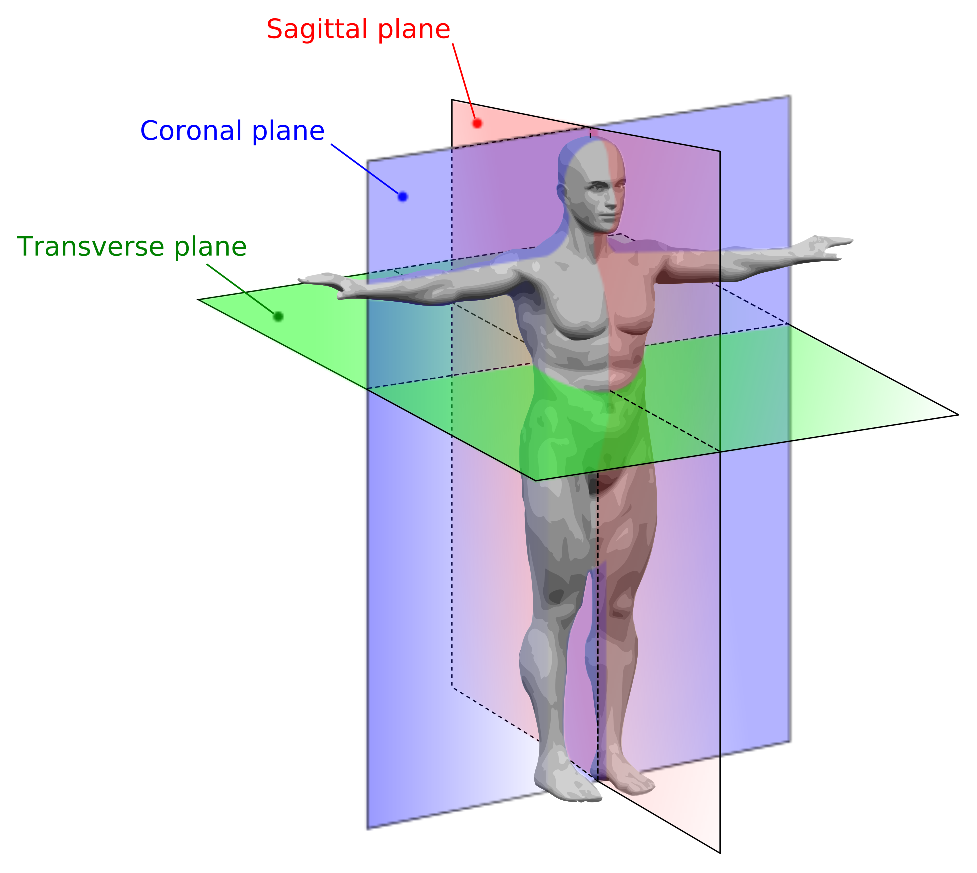
\includegraphics[width=0.7\textwidth]{spahittalPlae}
    \caption{SpahittaPlane}
    \label{fig:passivekneewalker}
\end{center}
\end{figure}




This chapter focuses on the motions in sagittal plane,  \dof s in coronal plane are discussed in Chapter~\ref{chap:highdor}.
More \dof s will introduce perturbations to our model, but will not change the basic motion characteristics and adaptation tendency.
They will make the ``symmetry'' not so perfect and may cause confusions in explaining the idea. thus the discussion is delayed.


The passive walking machine is shown in Figure~\ref{fig:passivekneewalker}.

\begin{figure}[!htbp]
  \begin{center}
    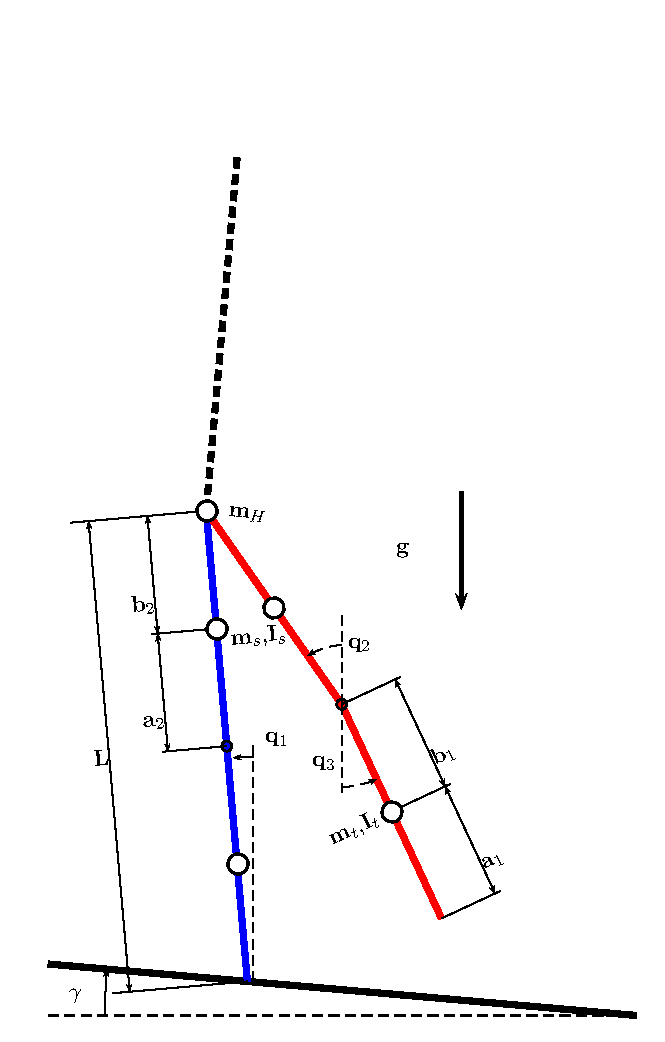
\includegraphics[width=0.7\textwidth]{PWI}
    \caption{A Passive Walking Model with Knee}
    \label{fig:passivekneewalker}
  \end{center}
\end{figure}



\subsection*{Dynamics}

Like the bouncing ball system, this system is hybrid\citep{ames2006categorical}, includes continuous and discrete dynamics[].
Passive walking with knees include four phases\citep{Chen2007}.
\begin{itemize}
\HiItem{Free Swing Phase}
The support leg (the blue one) is kept straight,during this phase the knee of the swing leg is bended, the thigh and shank swings freely.
\HiItem{Knee Strike Phase}
The knee joint of the swing leg has a limit.When the knee angle reach the limit,a collision happens.
After the collision, the swing leg is kept straight.
\HiItem{Knee Lock Swing Phase}
During this swing phase, both the swing and support leg are kept straight.
\HiItem{Heel Strike Phase}
When the heel of the swing leg hits the ground, a collision happens and after that the swing and support legs are switched.
\end{itemize}


The passive walker is modelled based on rigid body dynamics.
Dyanmic equations are developed based on Lagrange Mechanics~\citep{Goldstein2002}.
for details of calculating the dynamic equation, please reference\citep{Chen2007}



\begin{itemize}
\HiItem{Flying Phases}
For both the free and locked knee swing phases are described by the continuous dynamics.
Both equations are in the form of Equation~\ref{eq:flyequation}.
\begin{equation}
\label{eq:flyequation}
M(\mathbf{q}) \ddot{\mathbf{q}} + C(\mathbf{q,\qd})\dot{\mathbf{q}} + N(\mathbf{q}) = 0
\end{equation}
$q=[q_1,q_2,q_3]$,$\qd=[\dot{q_1},\dot{q_2},\dot{q_3}]$
where $M$ is the initial mass matrix, $C$ and $N$ are the centrifugal force matrix and gravity respectively. 
For Free Swing Phase,  $M$ and $C$ are $3$ by $3$ Matrix, $N$ is $3$ by $1$ vector.
for Knee Lock Phase, $M$ and $C$ are $2$ by $2$ Matrix, $N$ is $2$ by $1$ vector.
Put into the standard form, define $\state=[q,\qd]$, Equation~\ref{eq:flyequation} are transformed into Equation~\ref{eq:stateformpw}
Then the function is in the form.
\begin{equation}
\label{eq:stateformpw}
\dot{\state}=
-\left[ 
\begin{array}{cc}
\mathbf{1} &0\\
0 &M 
\end{array}
\right]^{-1}
\left[ 
\begin{array}{cc}
0 &\mathbf{1}\\
0 &C 
\end{array}
\right]\state
-\left[ 
\begin{array}{c}
\mathbf{0}\\
 N 
\end{array}
\right]
\end{equation}

\HiItem{The Strike Phases}
The knee strike and heel strike phases are modelled based on discrete dynamics.
collision equations are developed based on momentum perserving principle.
both collision equations are in the form of Equation~\ref{eq:collidequ}.
\begin{equation}
\label{eq:collidequ}
J^{+}\dot{\mathbf{q}}^{+} = J^{-}\dot{\mathbf{q}}^{-}
\end{equation}

where $J$ is the matrix of angular momentum inetia, the subscripts~$+,-$ represent after and before collision.
For Knees Strike,$J^-$ is a 3 by 2 Matrix, $J^+$ is 2 by 2 Matrix;
For Heel Strike, both $J^{+,-}$ are 2 by 2 Matrix.
\end{itemize}
For the components of each matrix, please refer to the appendix.







With special initial conditions, the passive walker can walk down the slope with a stable gait.
On the phase plot,  a limit cycle emergy. 
Figure ~\ref{fig:phasesmaker} shows the phase plot of one thigh for a stable walking cycle.
Four phases are marked, and Figure~\ref{fig:fwalkingphase} shows the the gait of four phases.

\begin{figure}[!htbp]
  \begin{center}
    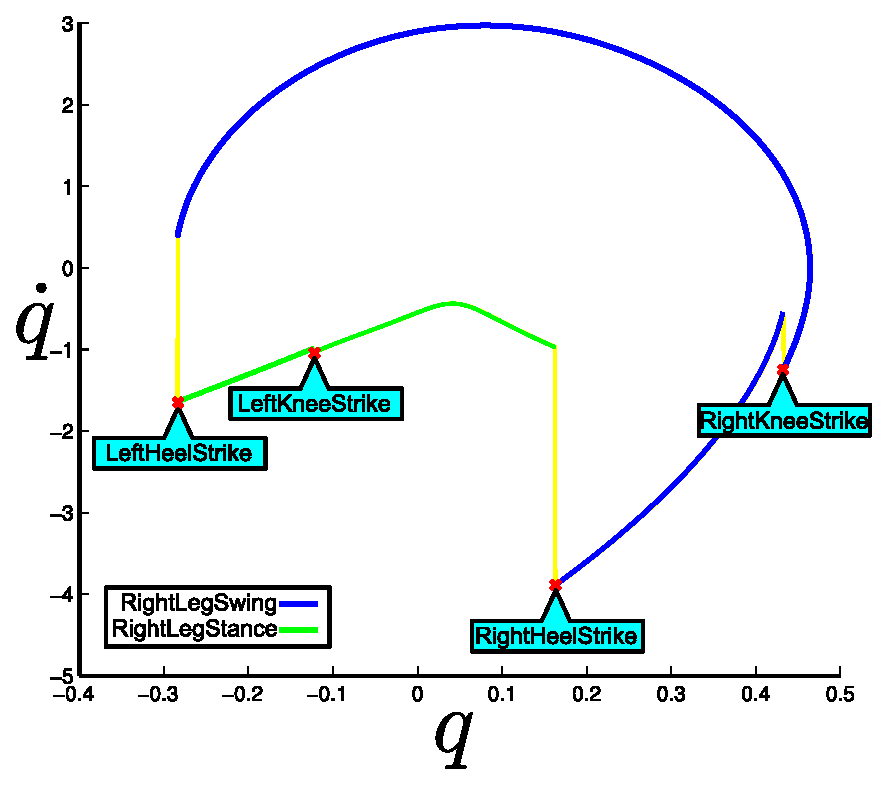
\includegraphics[width=0.7\textwidth]{walk_cycle_index}
    \caption{Four Phases Markered on a Walking Cycle}
    \label{fig:phasesmaker}
\end{center}
\end{figure}

\begin{figure}[!htbp]
  \begin{center}
      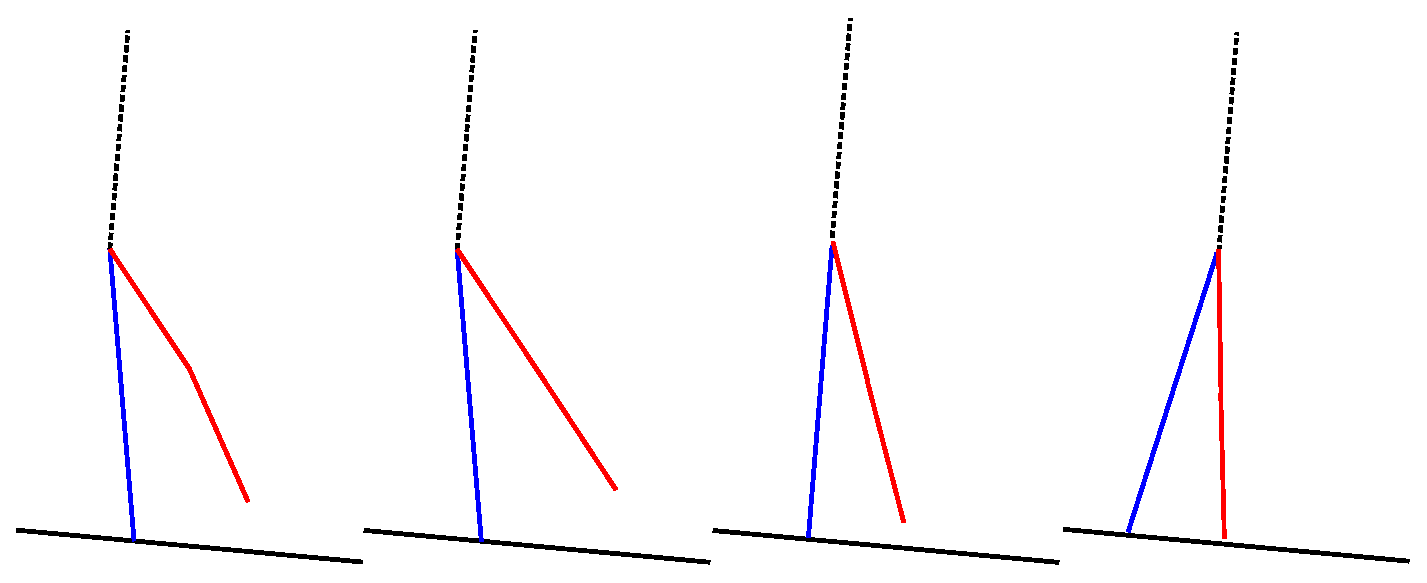
\includegraphics[width=0.7\textwidth]{Fourphase}
    \caption{The four phases in Walking}
    \label{fig:fwalkingphase}
\end{center}
\end{figure}








\section{Global Motor Control and Adaptive Gaits}

\subsection{Entrainment}
Neural oscillator Control  are applied to maintain the stability of limit cycle.

The output of neural oscillator worked as torque applied at hip angel (angle between the two thighs).
The dynamics are shown in Equation~\ref{eq:neuralwalk}
\begin{equation}
\label{eq:neuralwalk}
M(\mathbf{q}) \ddot{\mathbf{q}} + C(\mathbf{q,\qd})\dot{\mathbf{q}} + N(\mathbf{q}) = D\uout
\end{equation}
For the knee lock phase $D=[1,-1]^T$.
For the knee free phase, $D=[1,-1,0]^T$(acting on the difference between the two thighs, not effect the knee)

the input signal is the hip angle,
we have 
\[
	\uin=\hin(q_1-q_2)
\]

when the drive force is small, the limit cycle of entrainment system is similar to the passive one original passive one.
Both limit cycles are shown in Figure~\ref{fig:passivegaitlimitcycle} and Figure~\ref{fig:entrainmentgaitlimitcyle}.
Walking gatis are shown in Figure~\ref{fig:entrainmentgait} and Figure~\ref{fig:passivegait}.




\begin{figure}[!htbp]
  \begin{center}
    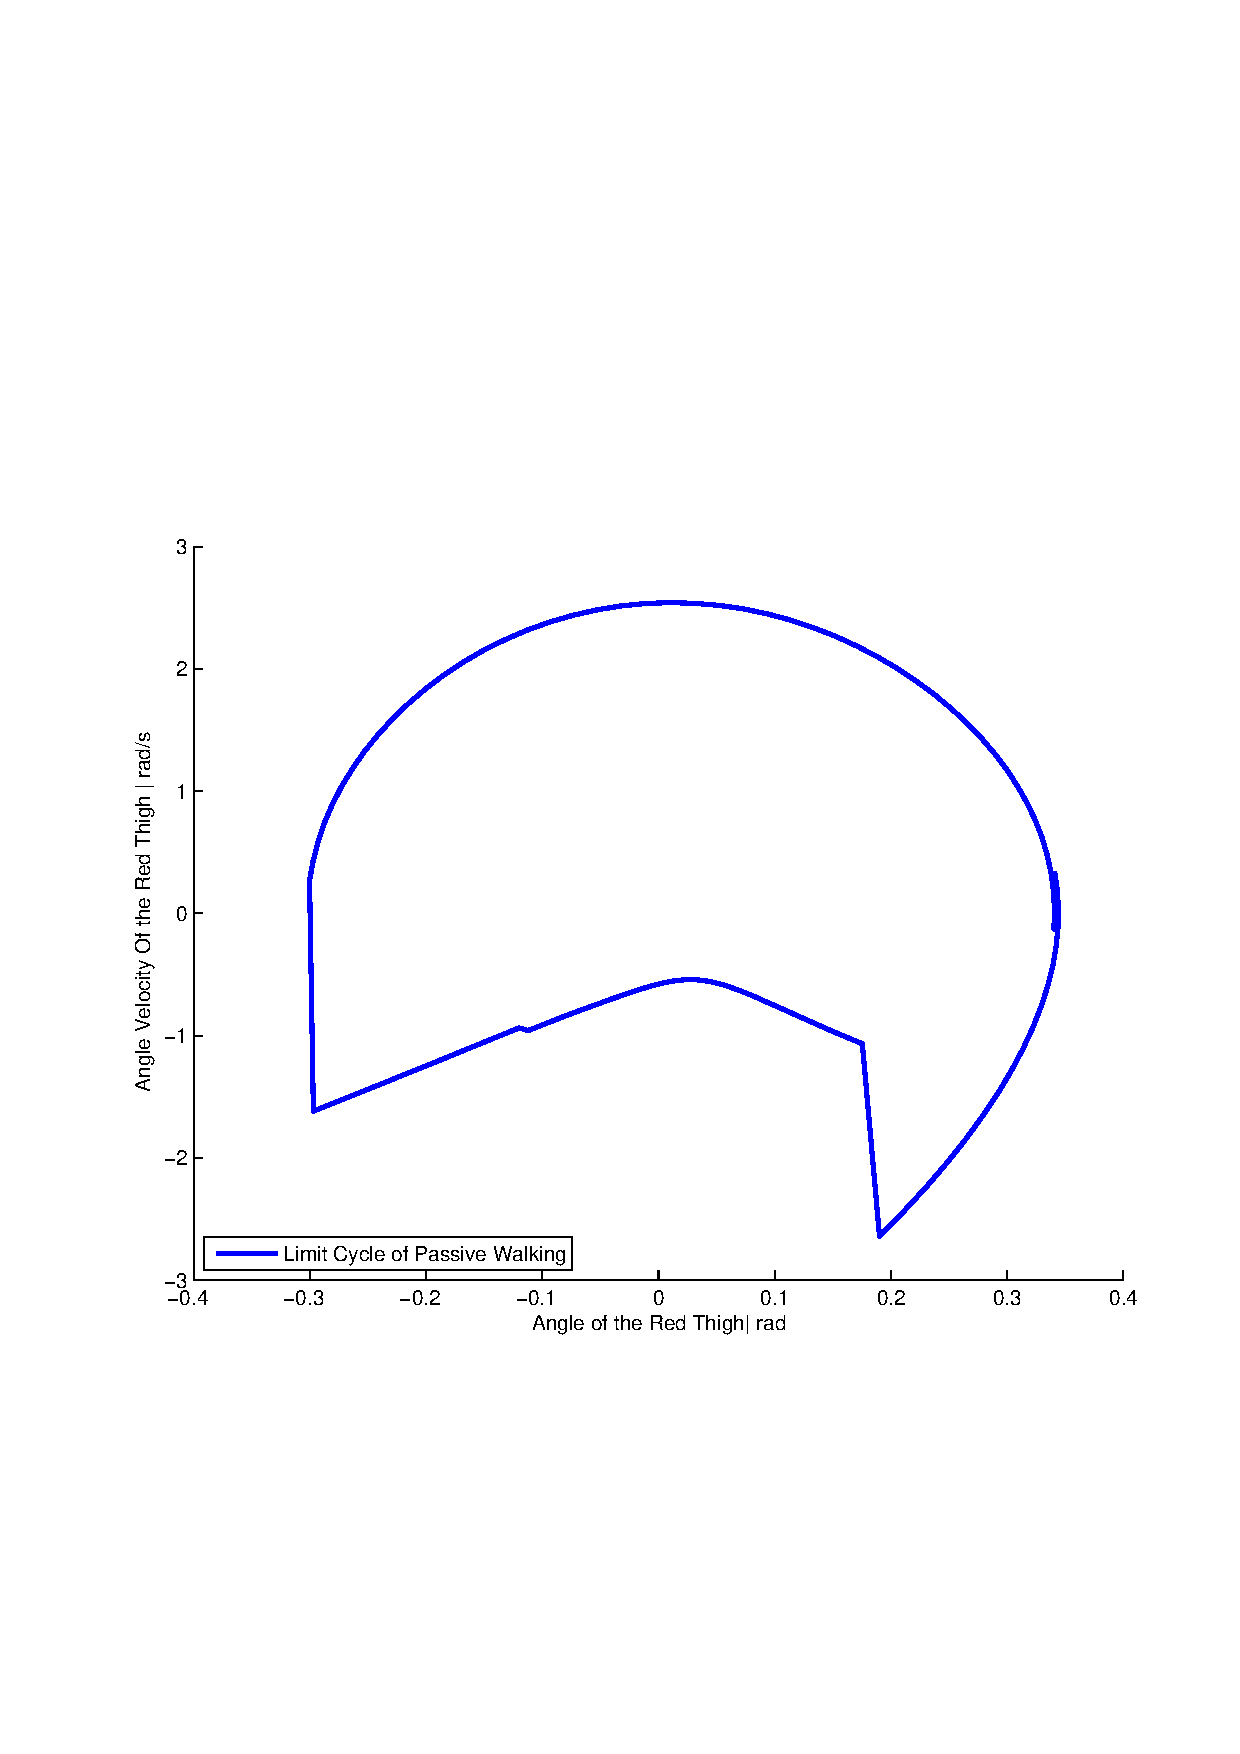
\includegraphics[width=0.7\textwidth]{PassiveWalkingLimitCycle}
    \caption{Limit Circle And Different Phase in Passive Walking}
    \label{fig:passivegaitlimitcycle}
\end{center}
\end{figure}


\begin{figure}[!htbp]
  \begin{center}
      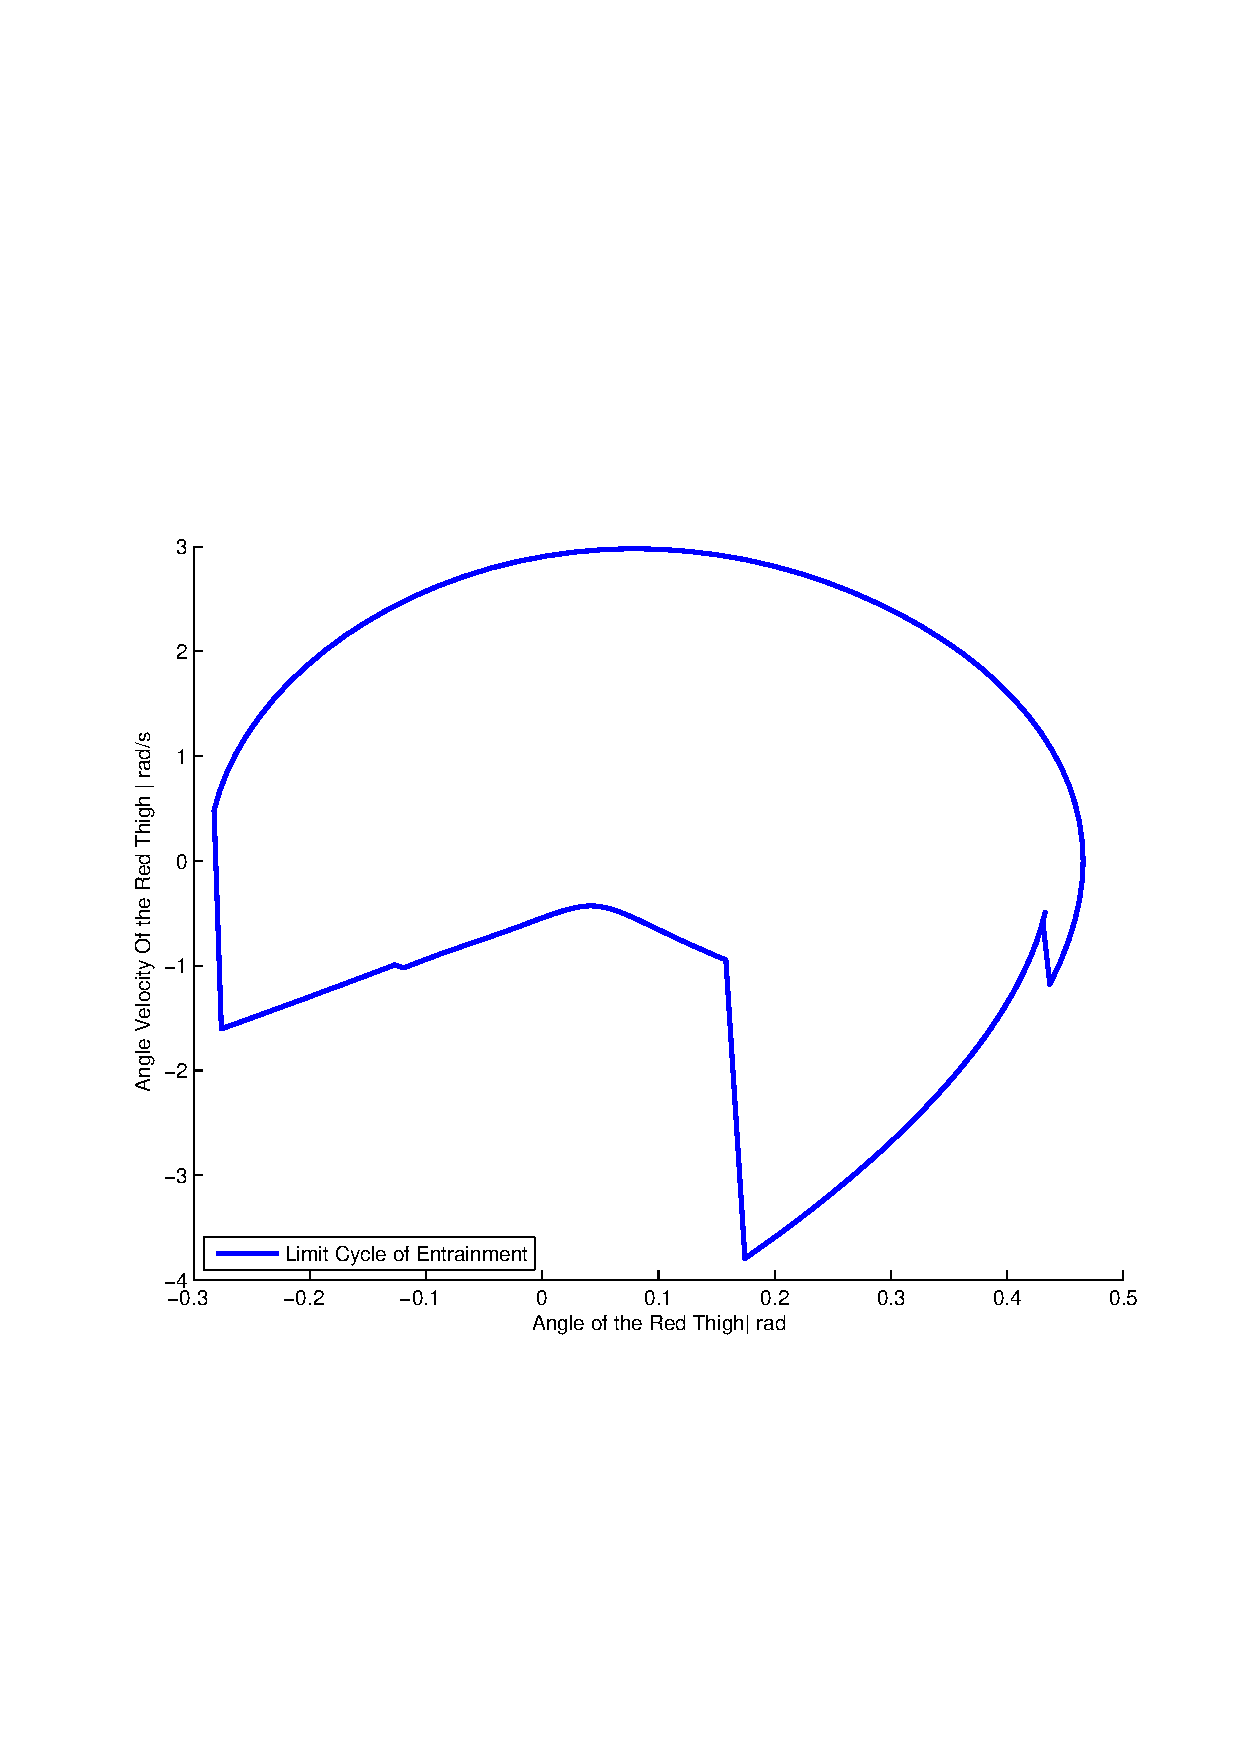
\includegraphics[width=0.7\textwidth]{NeuralWalkingLimitCycle}
    \caption{The gait with neural controller}
    \label{fig:entrainmentgaitlimitcyle}
\end{center}
\end{figure}

\begin{figure}[!htbp]
  \begin{center}
     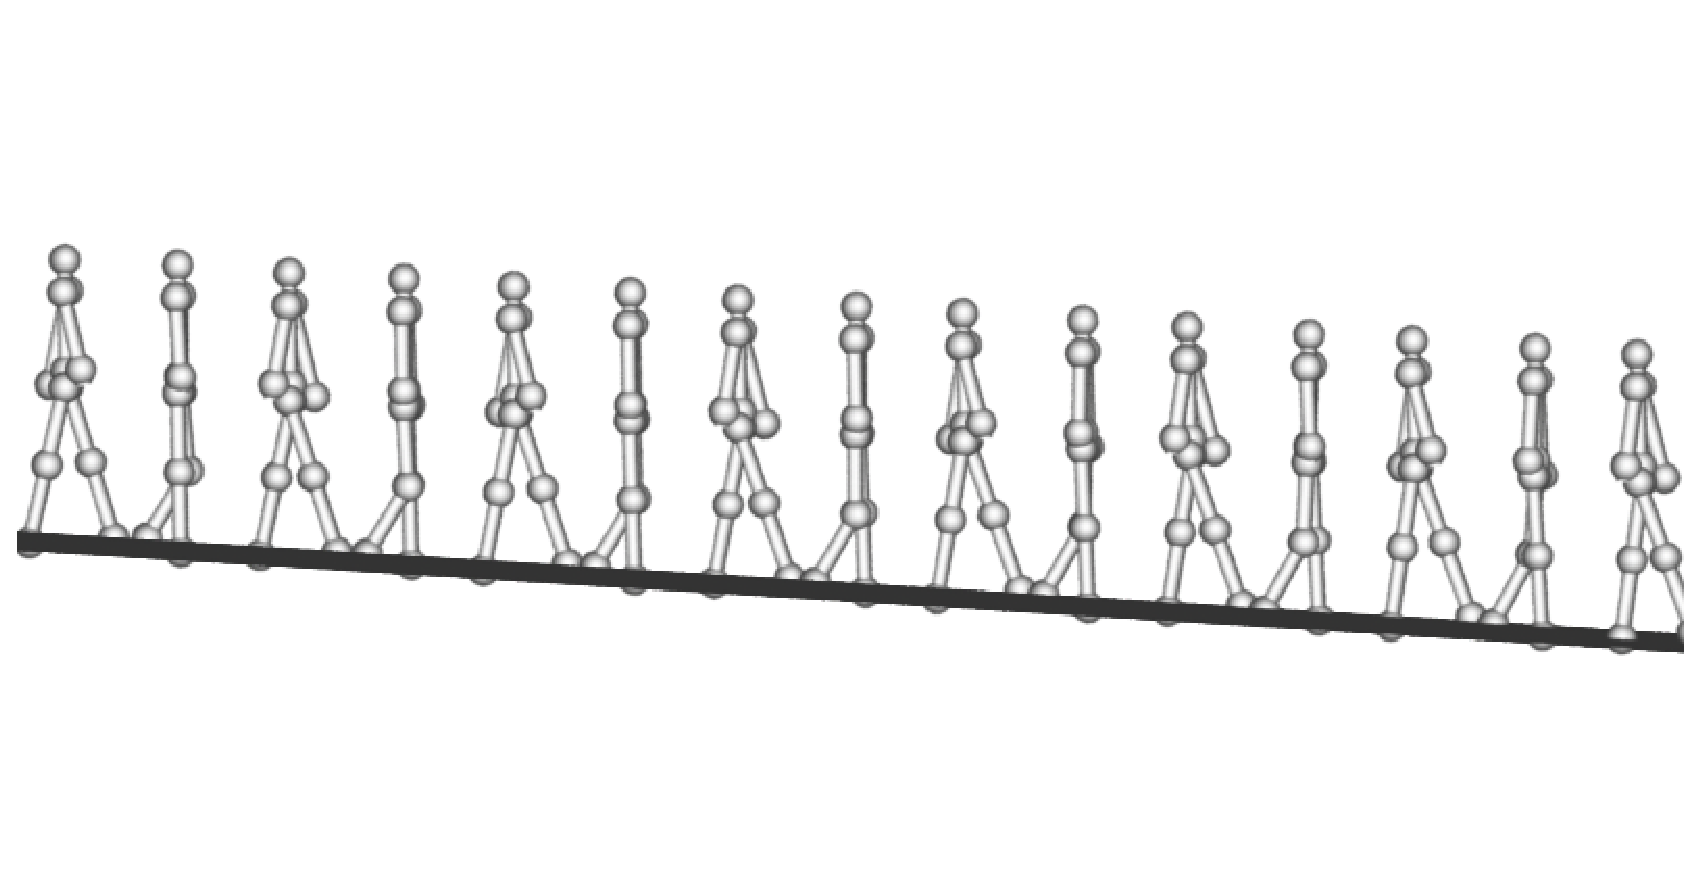
\includegraphics[width=0.7\textwidth]{PassiveGait}
    \caption{The Passive Walking Gait}
    \label{fig:passivegait}
\end{center}
\end{figure}

\begin{figure}[!htbp]
  \begin{center}
     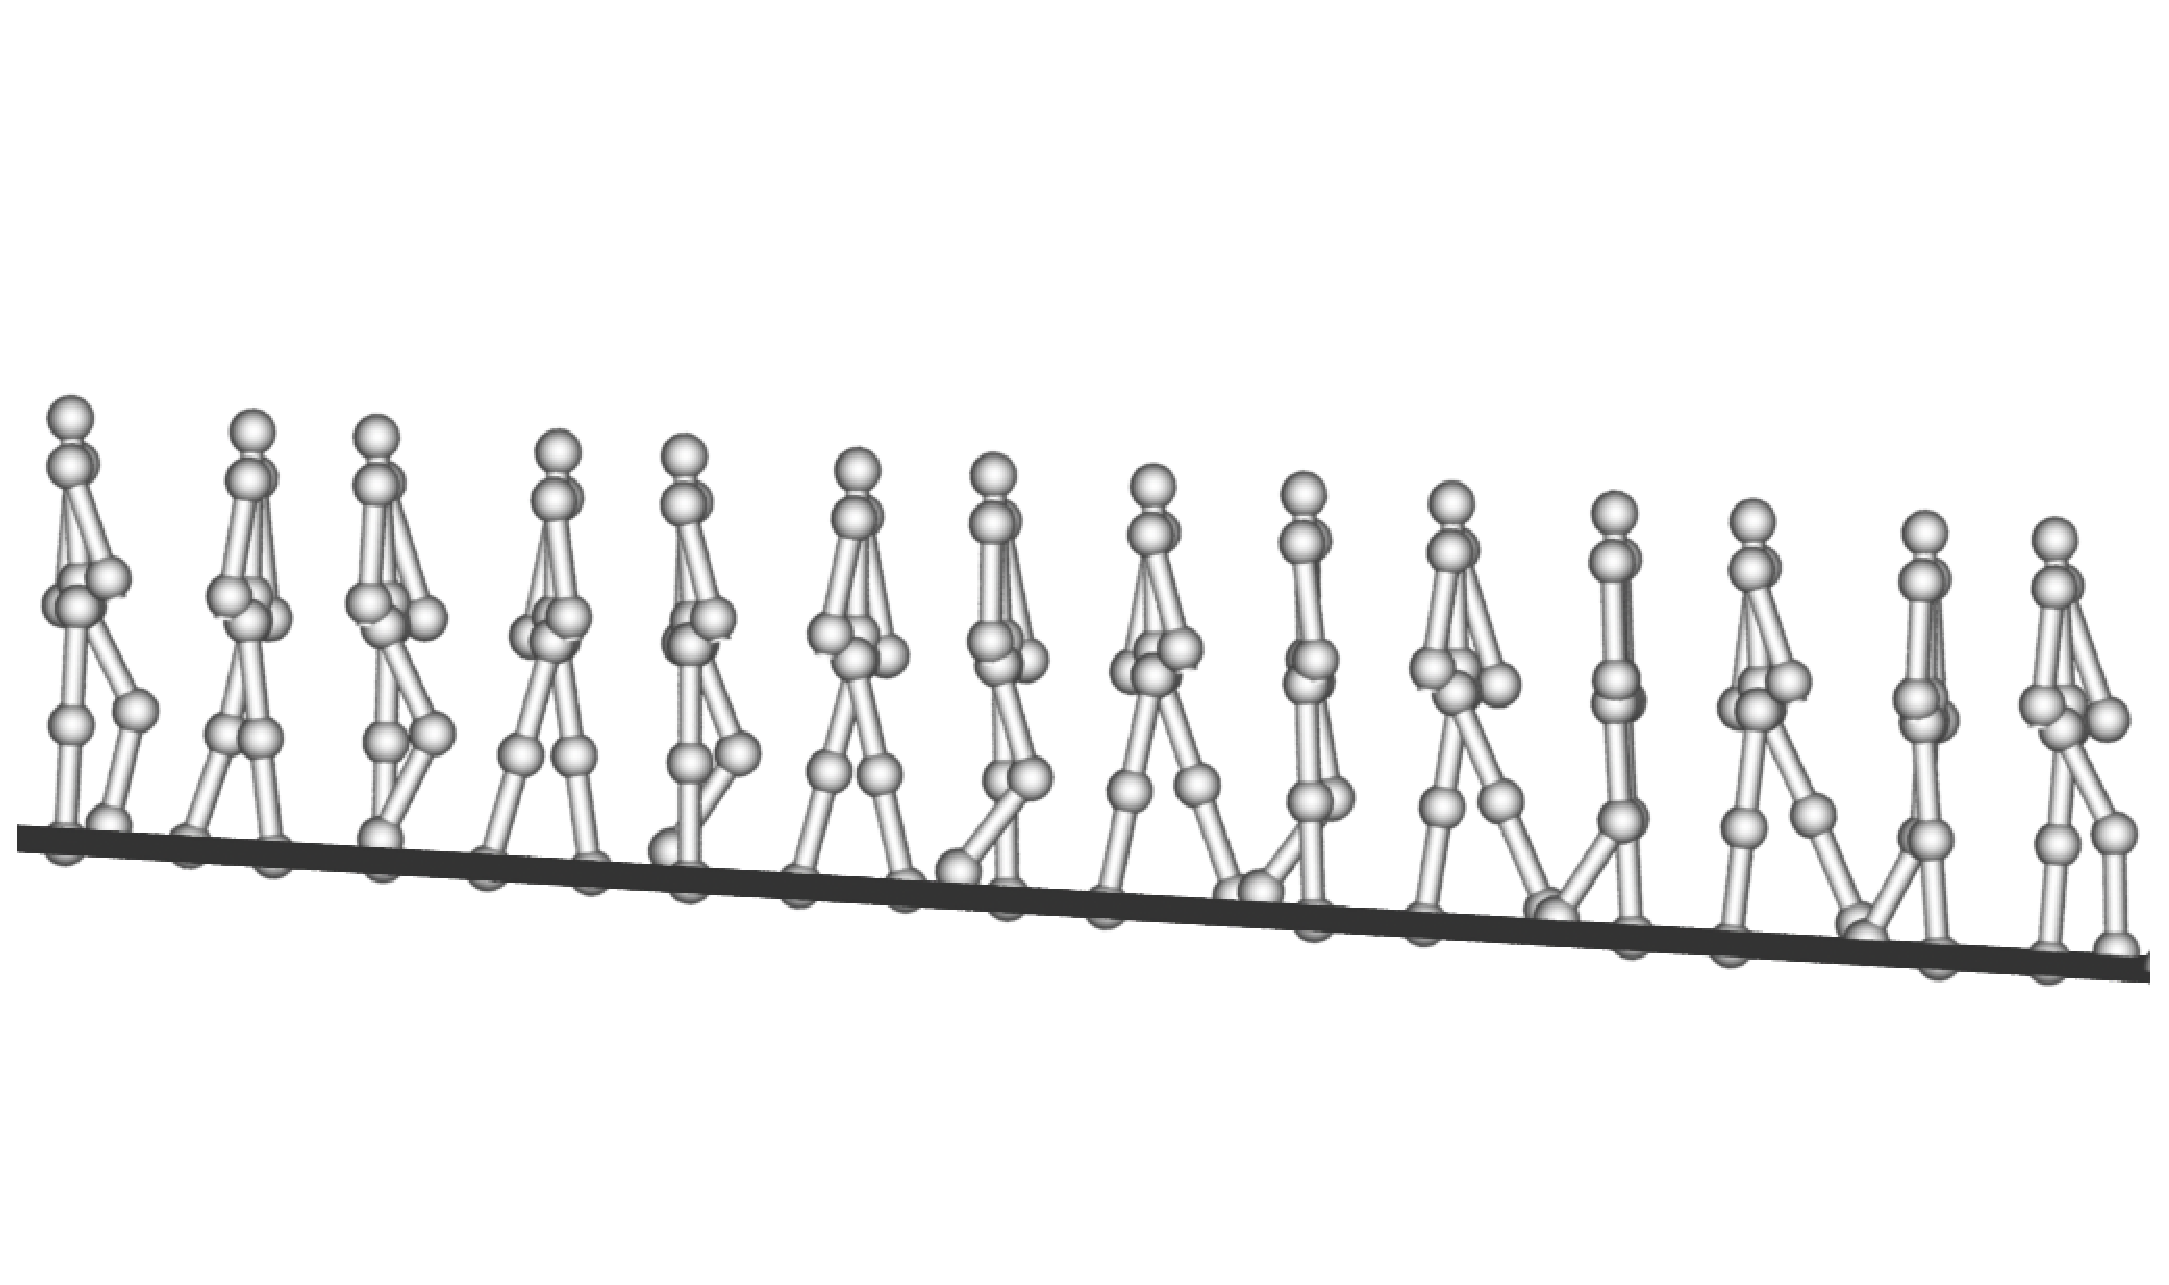
\includegraphics[width=0.7\textwidth]{neuralWalk}
    \caption{Passive Walking with Neural Control}
    \label{fig:entrainmentgait}
\end{center}
\end{figure}

\subsection{Stabilility}

Neural oscillator  boosts structrual stability of walking. 
The passive walking can not be maintained on plane, structure perturbation from slope angle violate the topology, limit cycle does not exist any more.
The stepsize descrease every step, after several steps, and the walker will stop or fall over,as shown in Figure~\ref{fig:passivegaitplane}
After coupling with neural oscillator, the  walker maintain the gait with a small stepsize,as shonw in Figure~\ref{fig:neuralwalkinggait}.
To maintain the energy efficient property of natural motion, $\uout$ is limited to small, thus maintain a small stepsize,as shown in Figure~\ref{fig:entrainmentLimitCycleOnPlane}.

\begin{figure}[!htbp]
  \begin{center}
    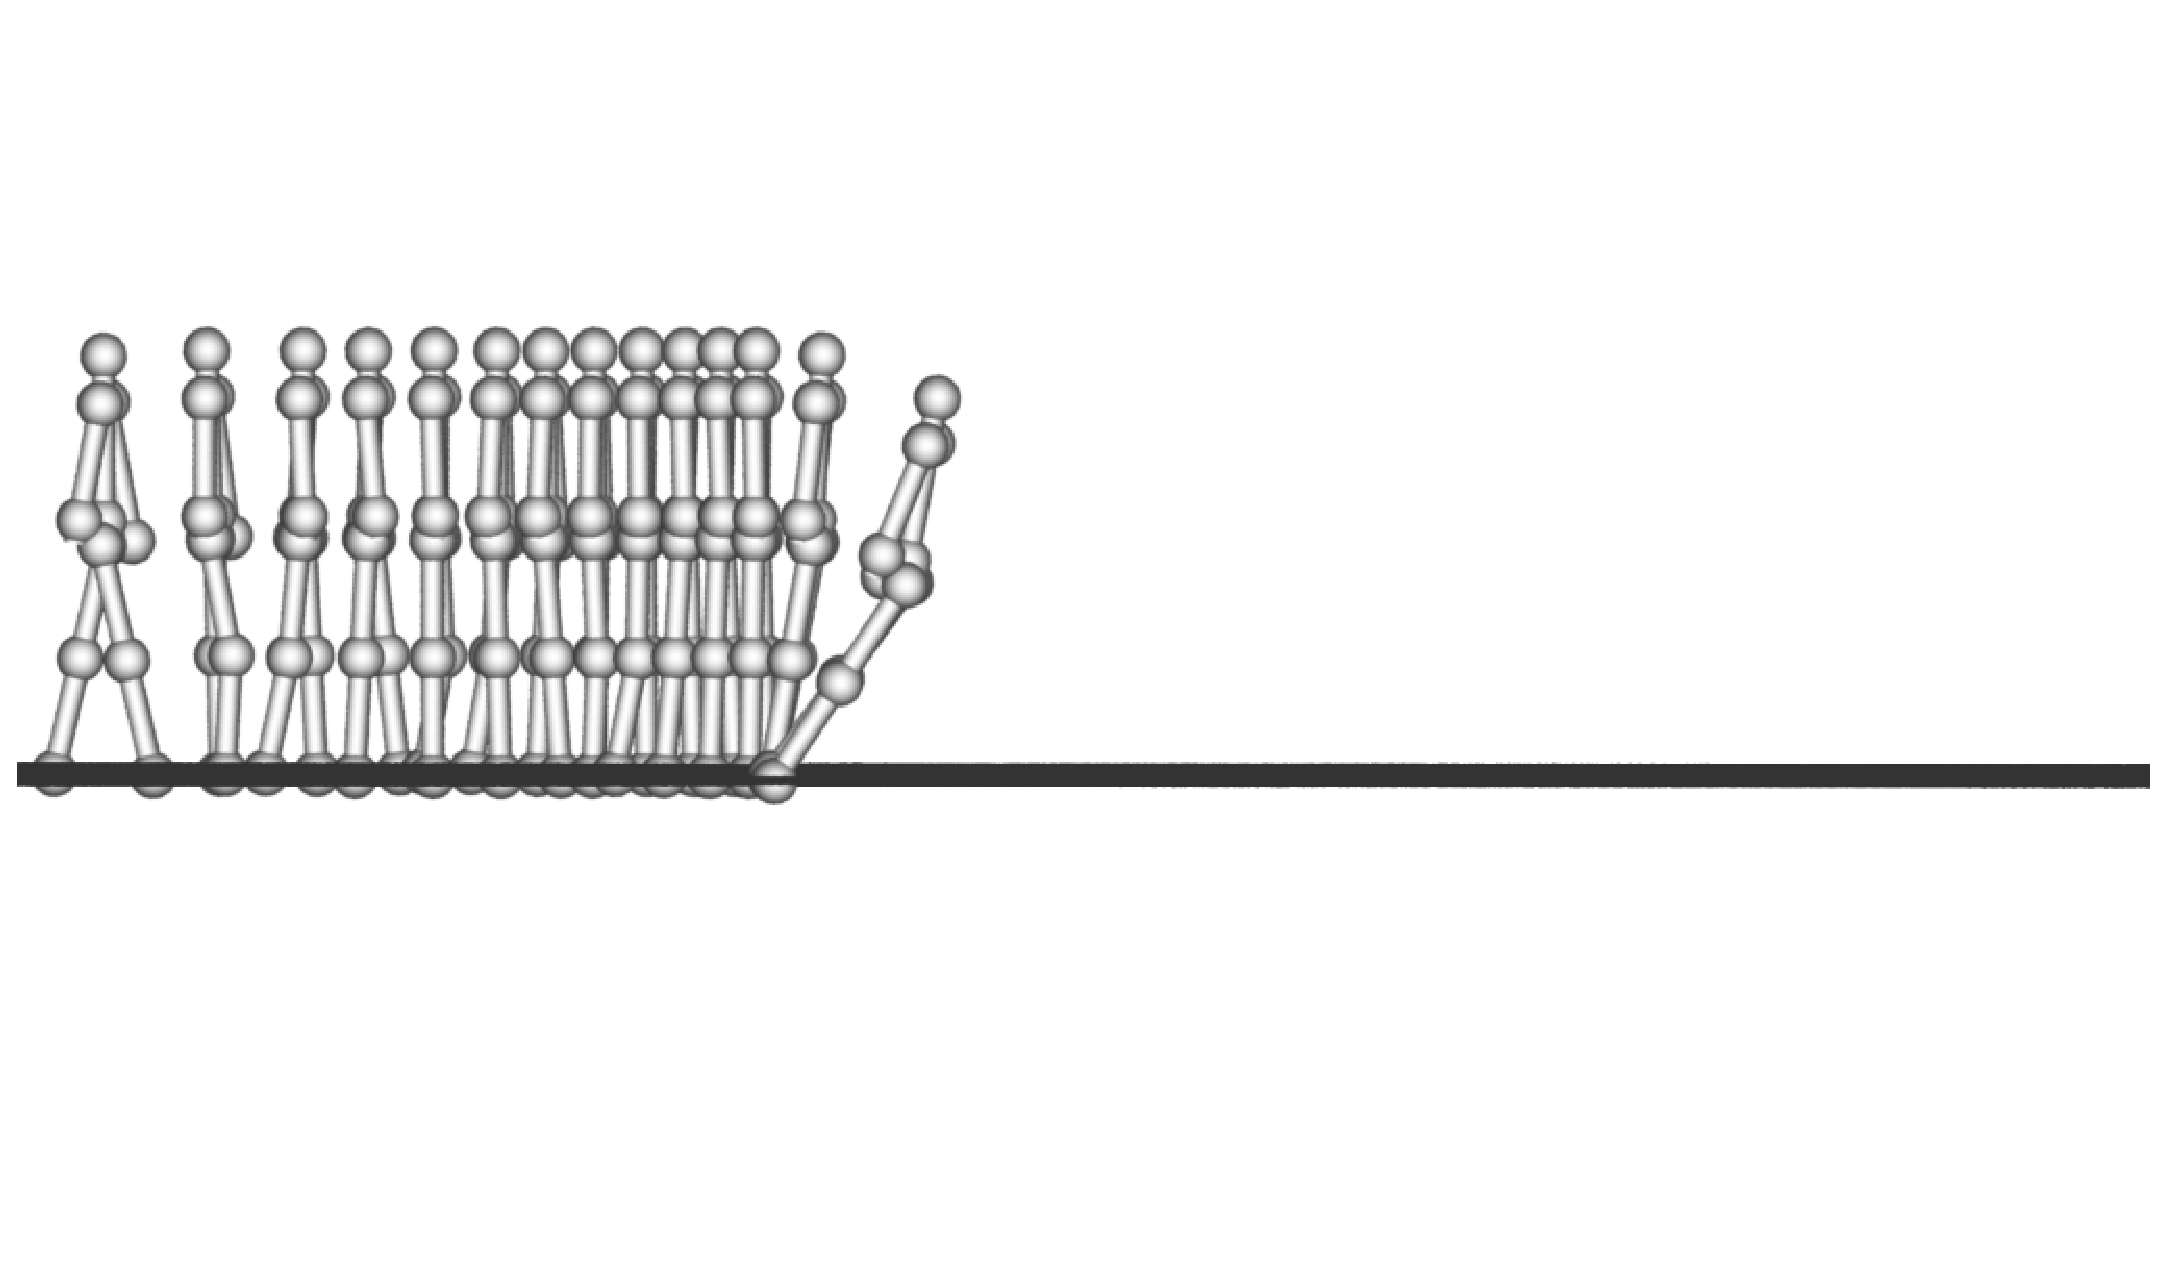
\includegraphics[width=0.7\textwidth]{PassiveOnPlane}
    \caption{Passive On Plain}
    \label{fig:passivegaitplane}
\end{center}
\end{figure}

\begin{figure}[!htbp]
  \begin{center}
     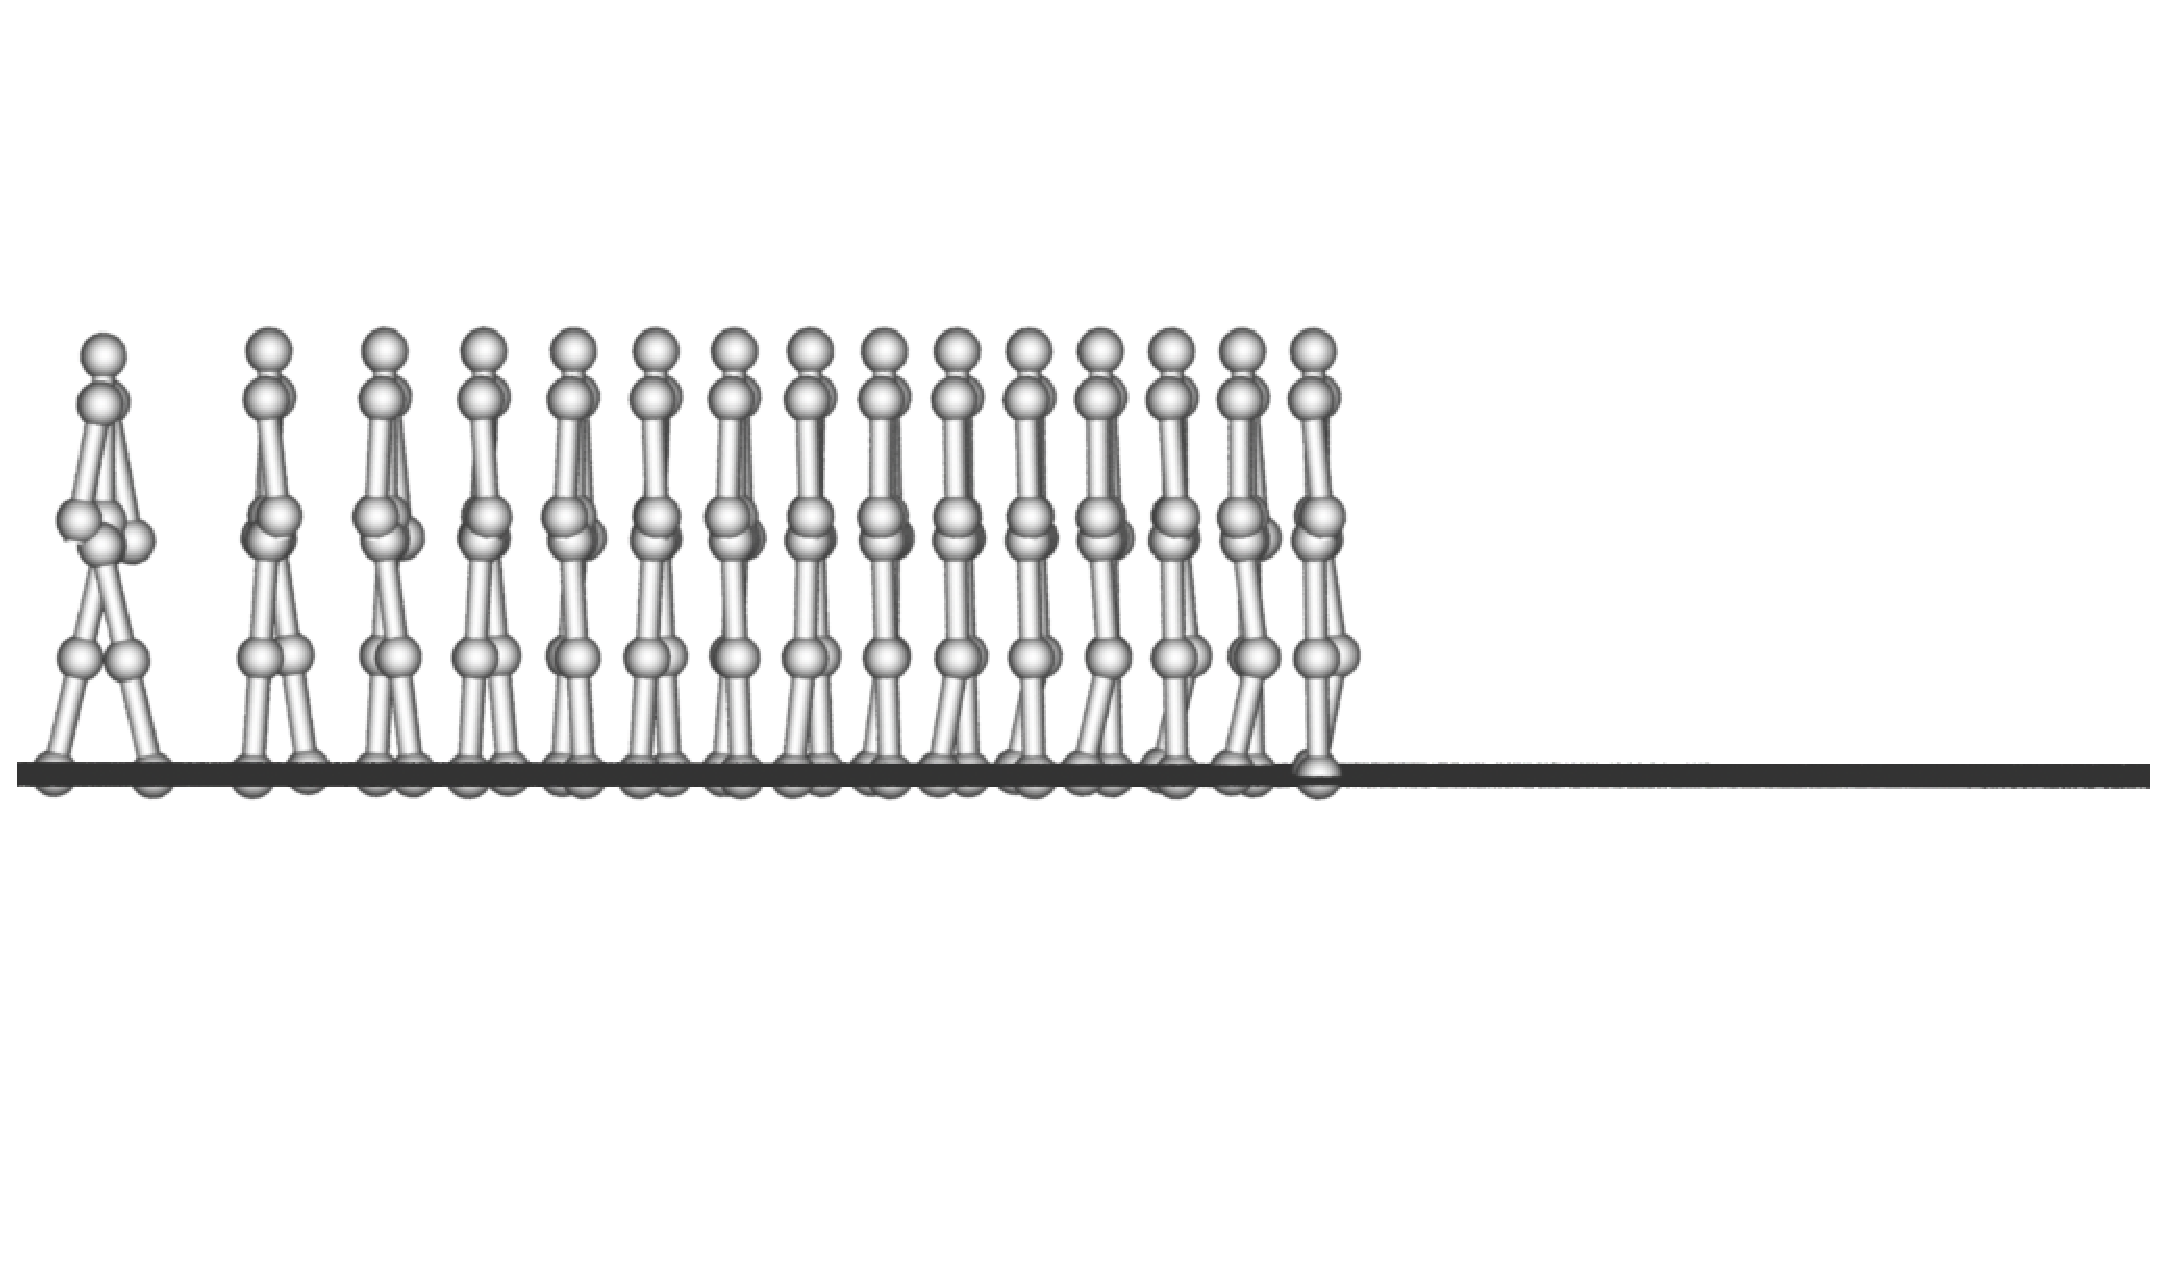
\includegraphics[width=0.7\textwidth]{NeuralWalkingPlane}
    \caption{Entraint Gait On Plane}
    \label{fig:neuralwalkinggait}
\end{center}
\end{figure}

\begin{figure}[!htbp]
  \begin{center}
      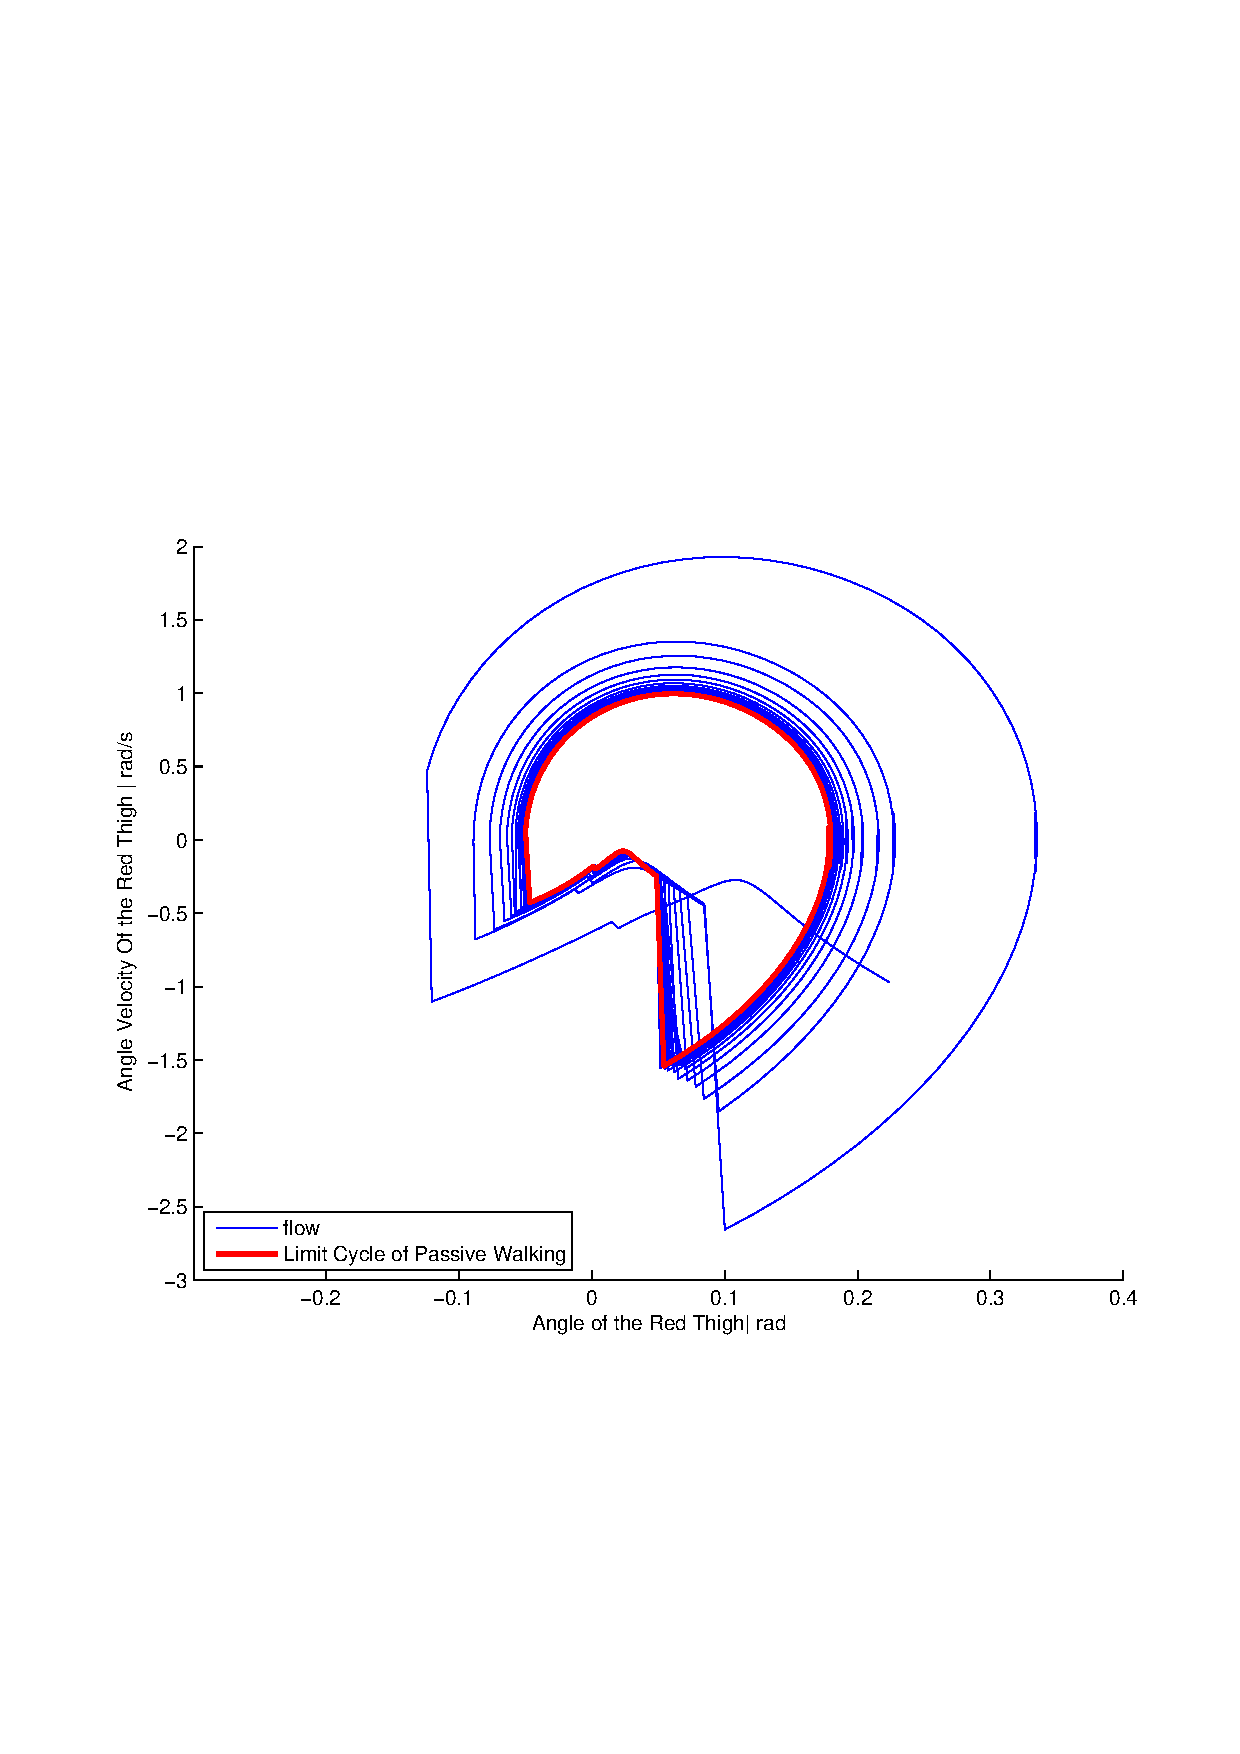
\includegraphics[width=0.7\textwidth]{NeuralPlaneCycle}
    \caption{Limit Cycle of entrainment gait on plane}
    \label{fig:entrainmentLimitCycleOnPlane}
\end{center}
\end{figure}



For Figure~\ref{fig:entrainmentLimitCycleOnPlane}, the initial postion is far from the limit cycle, this shows that the basin of attraction has been enlarged.
State perturbation applied to generate pushed or pulled walking gaits as shown in Figure~\ref{fig:PushGait} and Figure~\ref{fig:PullGait}.
And Figure~\ref{fig:PushGaitPlot} and Figure~\ref{fig:PullGaitPhasePlot} show the flow convergence of the limit cycle.

\begin{figure}[!htbp]
  \begin{center}
      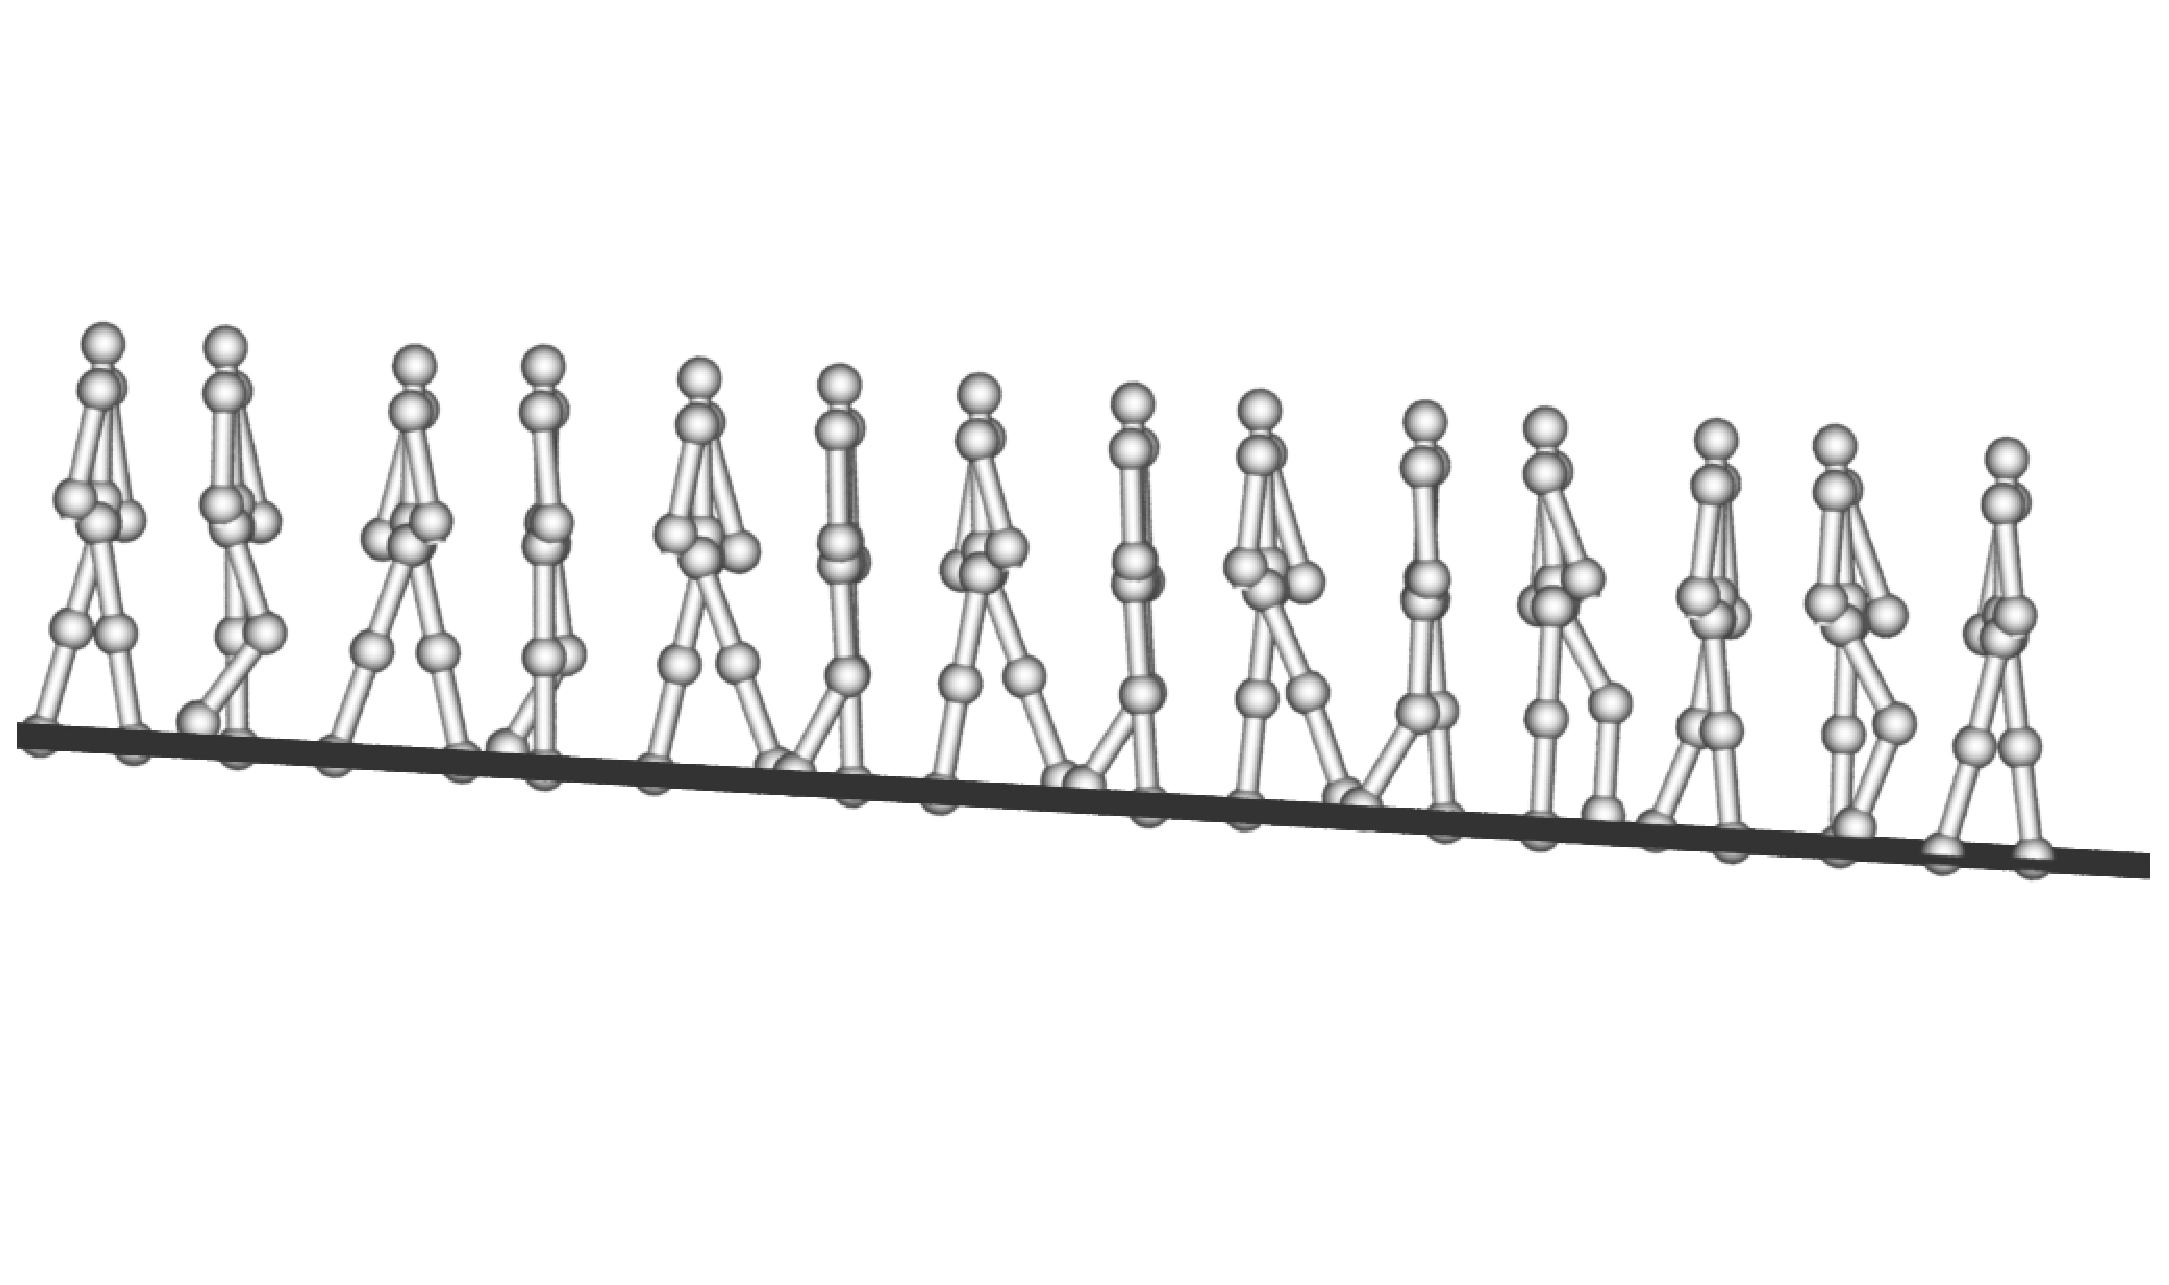
\includegraphics[width=0.7\textwidth]{PushGait}
    \caption{The Push Perturbated Gait}
    \label{fig:PushGait}
\end{center}
\end{figure}


\begin{figure}[!htbp]
  \begin{center}
      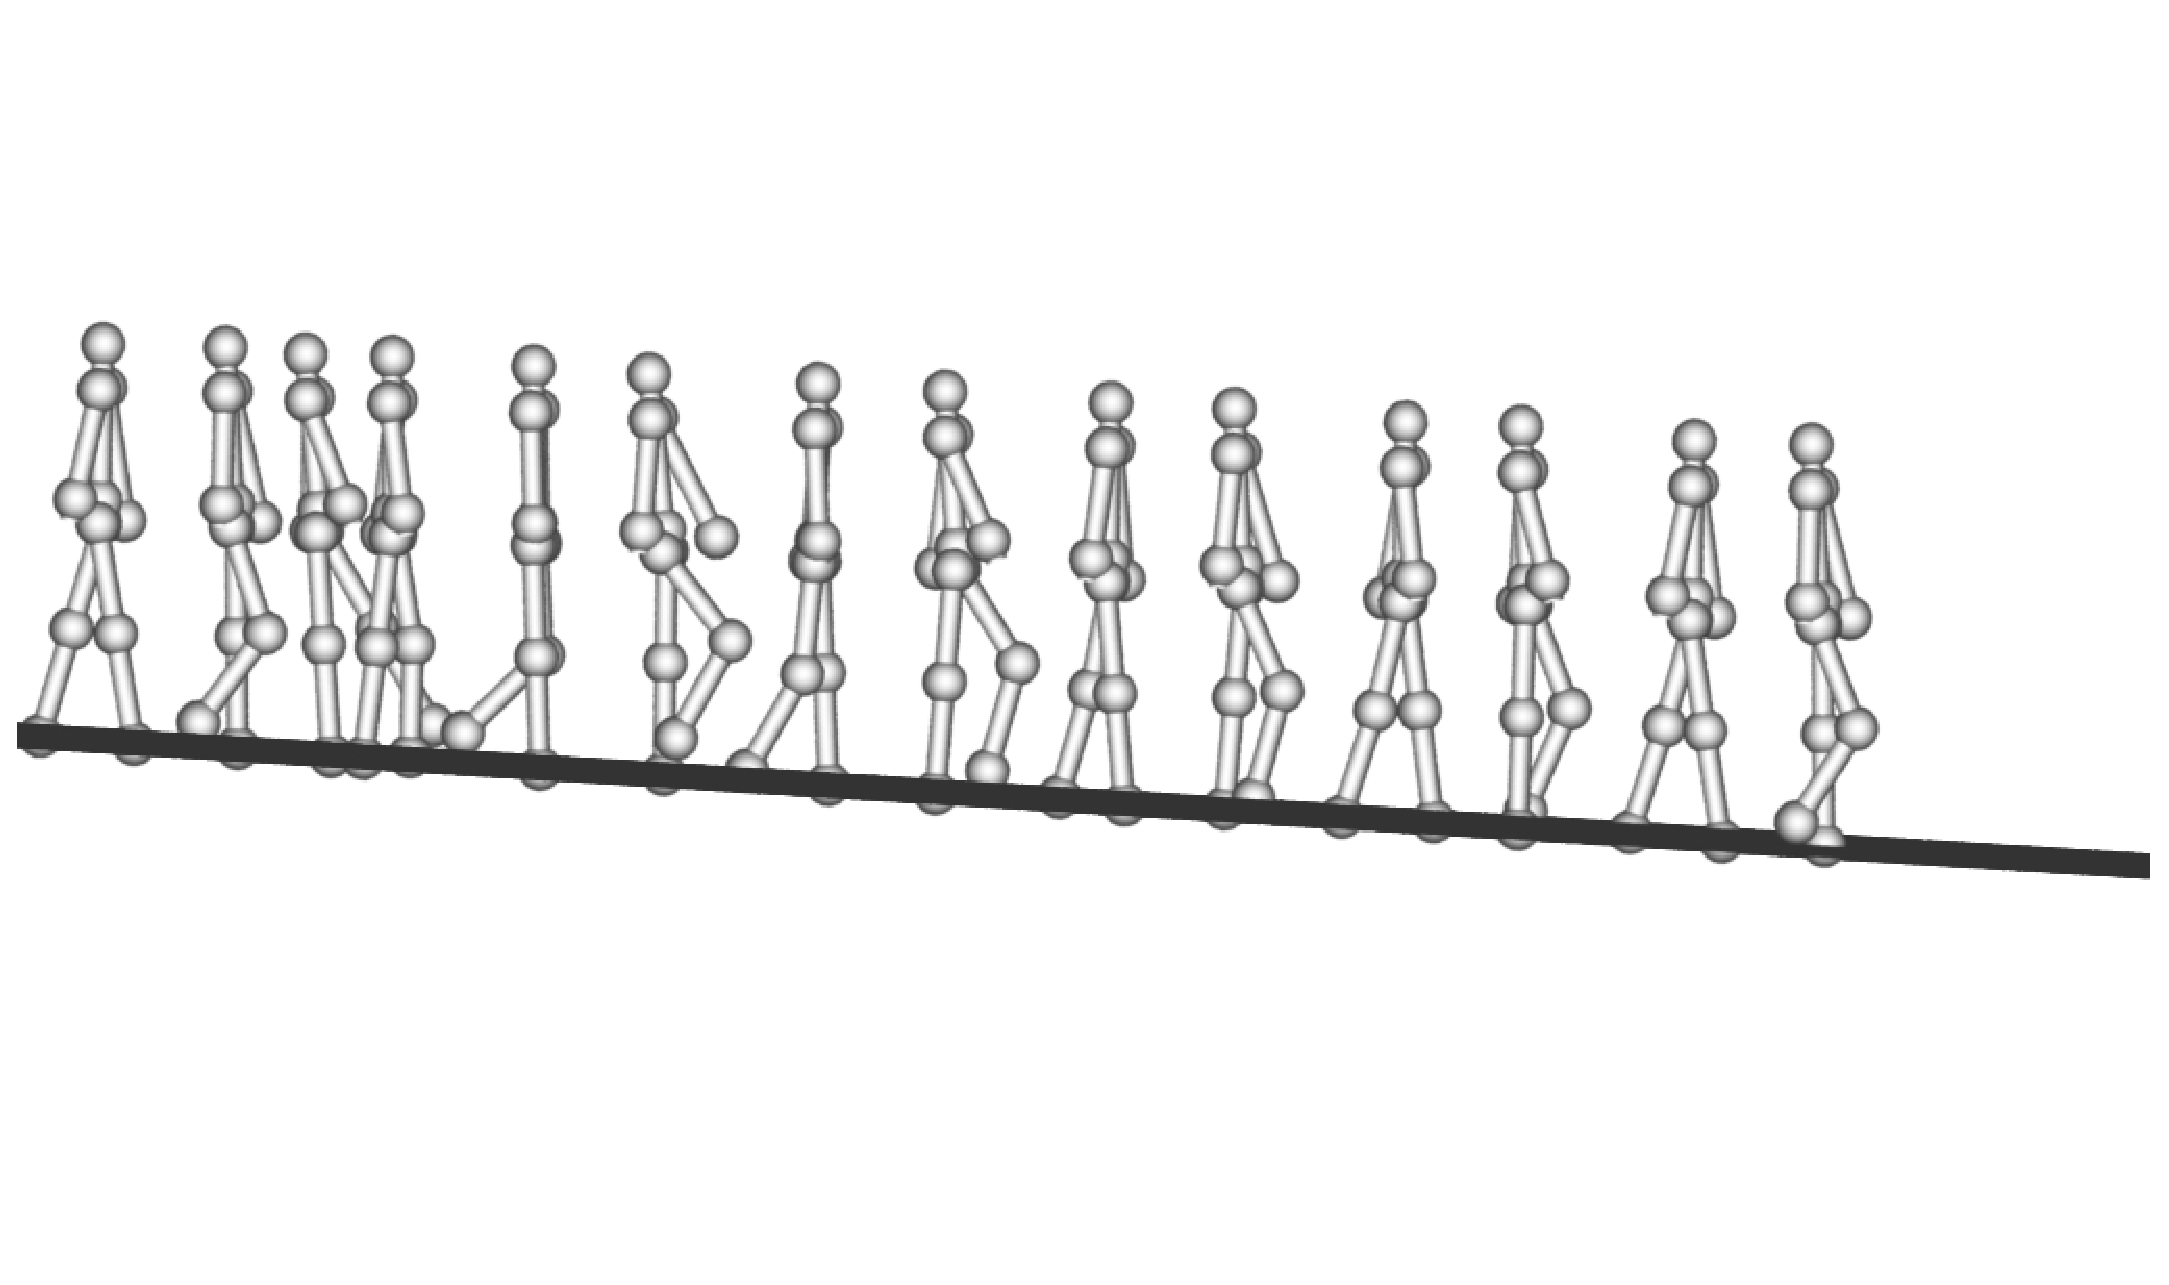
\includegraphics[width=0.7\textwidth]{PullGait}
    \caption{The Pull Perturbated Gait}
    \label{fig:PullGait}
\end{center}
\end{figure}


\begin{figure}[!htbp]
  \begin{center}
      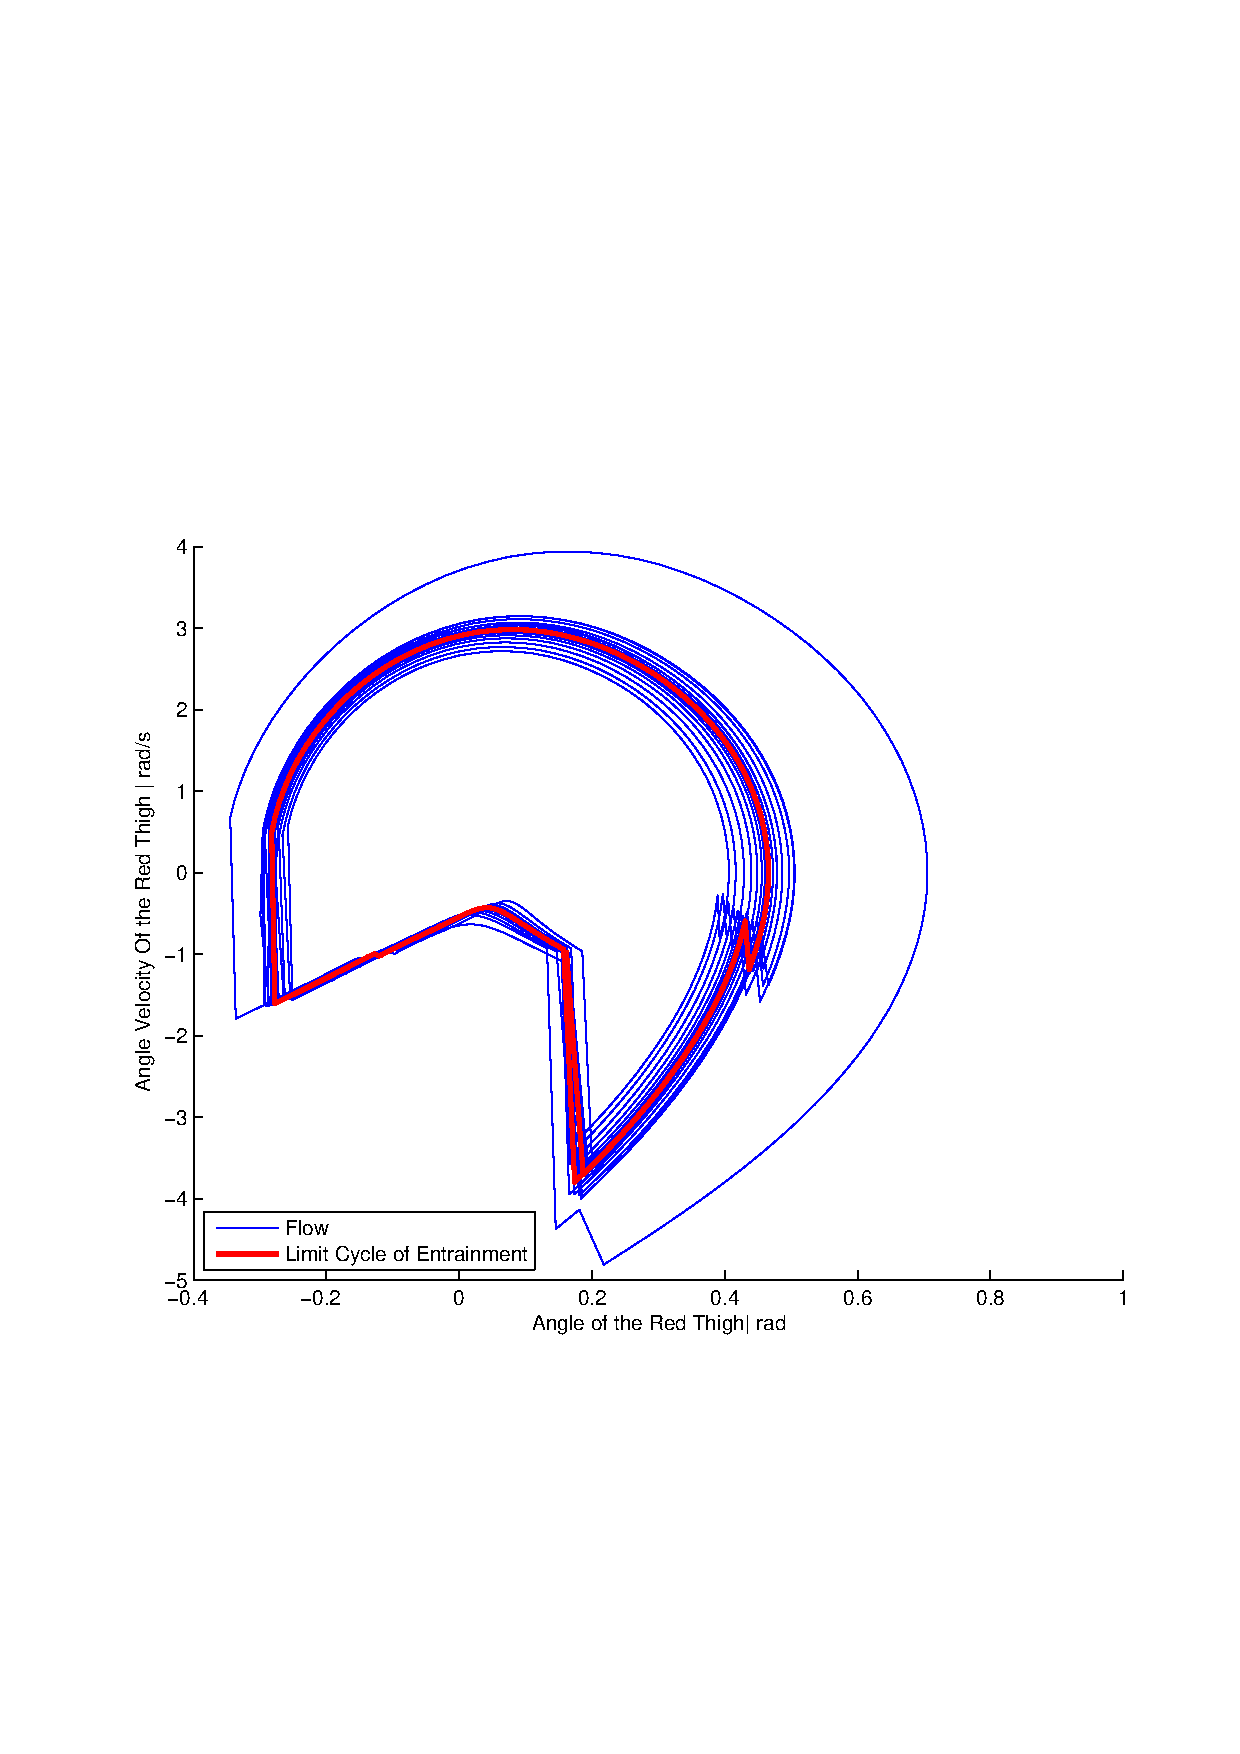
\includegraphics[width=0.7\textwidth]{PushWalkingPhasePlot}
    \caption{The Pushed Gait Phase Plot}
    \label{fig:PushGaitPlot}
\end{center}
\end{figure}


\begin{figure}[!htbp]
  \begin{center}
      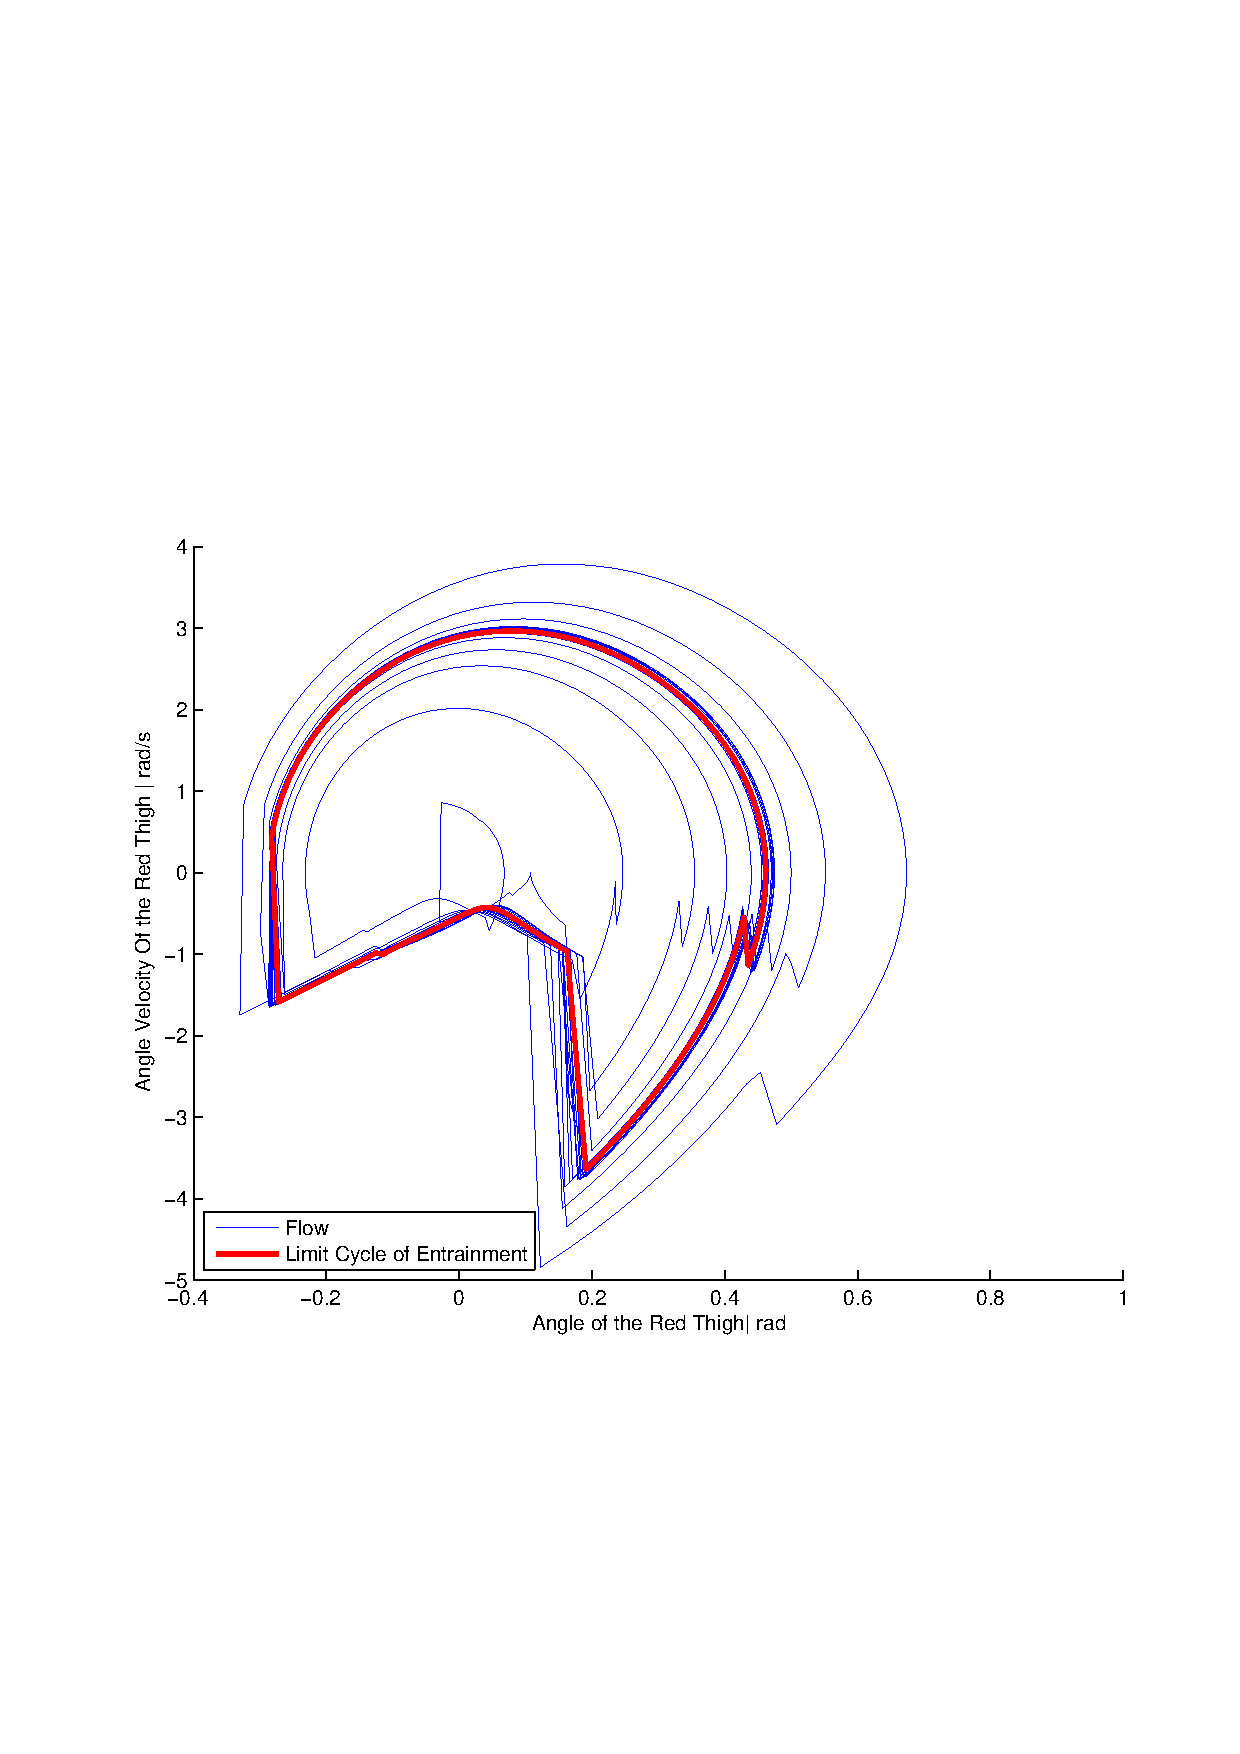
\includegraphics[width=0.7\textwidth]{PullWalkingPhasePlot}
    \caption{The Pulled Gait Phase Plot}
    \label{fig:PullGaitPhasePlot}
\end{center}
\end{figure}


Also the change the initial stepsize, the walker will adjust it automatically.
Figure~\ref{fig:bigStepIni} and Figure~\ref{fig:smallStepini} show the gaits.
Figure~\ref{fig:bigstepiniGaitPlot} and Figure~\ref{fig:smallstepiniPhasePlot} show the phase plot.

\begin{figure}[!htbp]
  \begin{center}
      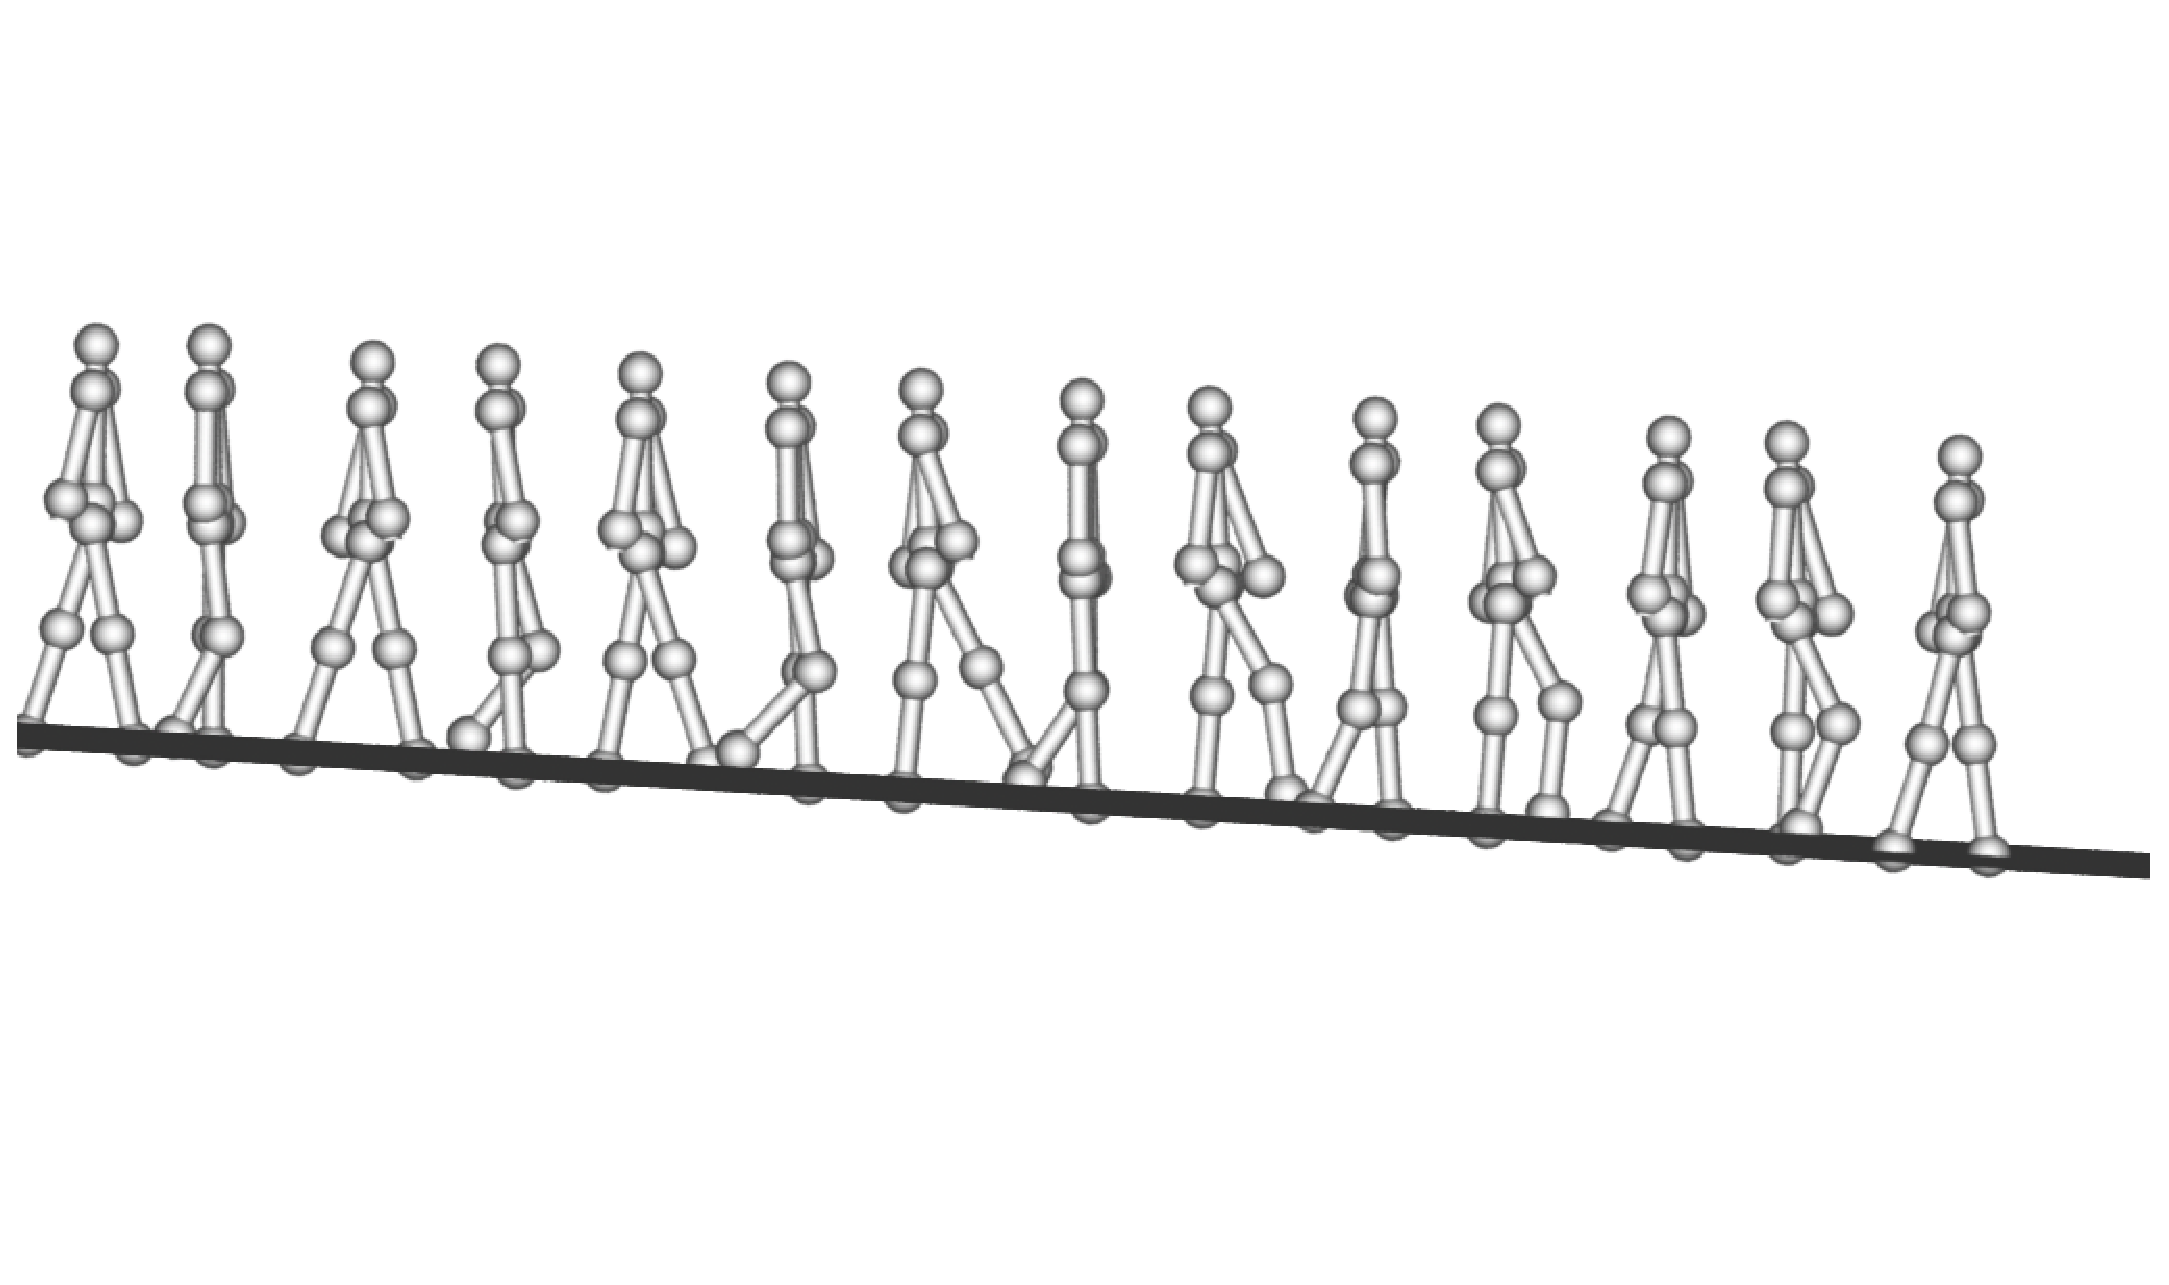
\includegraphics[width=0.7\textwidth]{BigStep}
    \caption{Big Initial Step Size}
    \label{fig:bigStepIni}
\end{center}
\end{figure}


\begin{figure}[!htbp]
  \begin{center}
      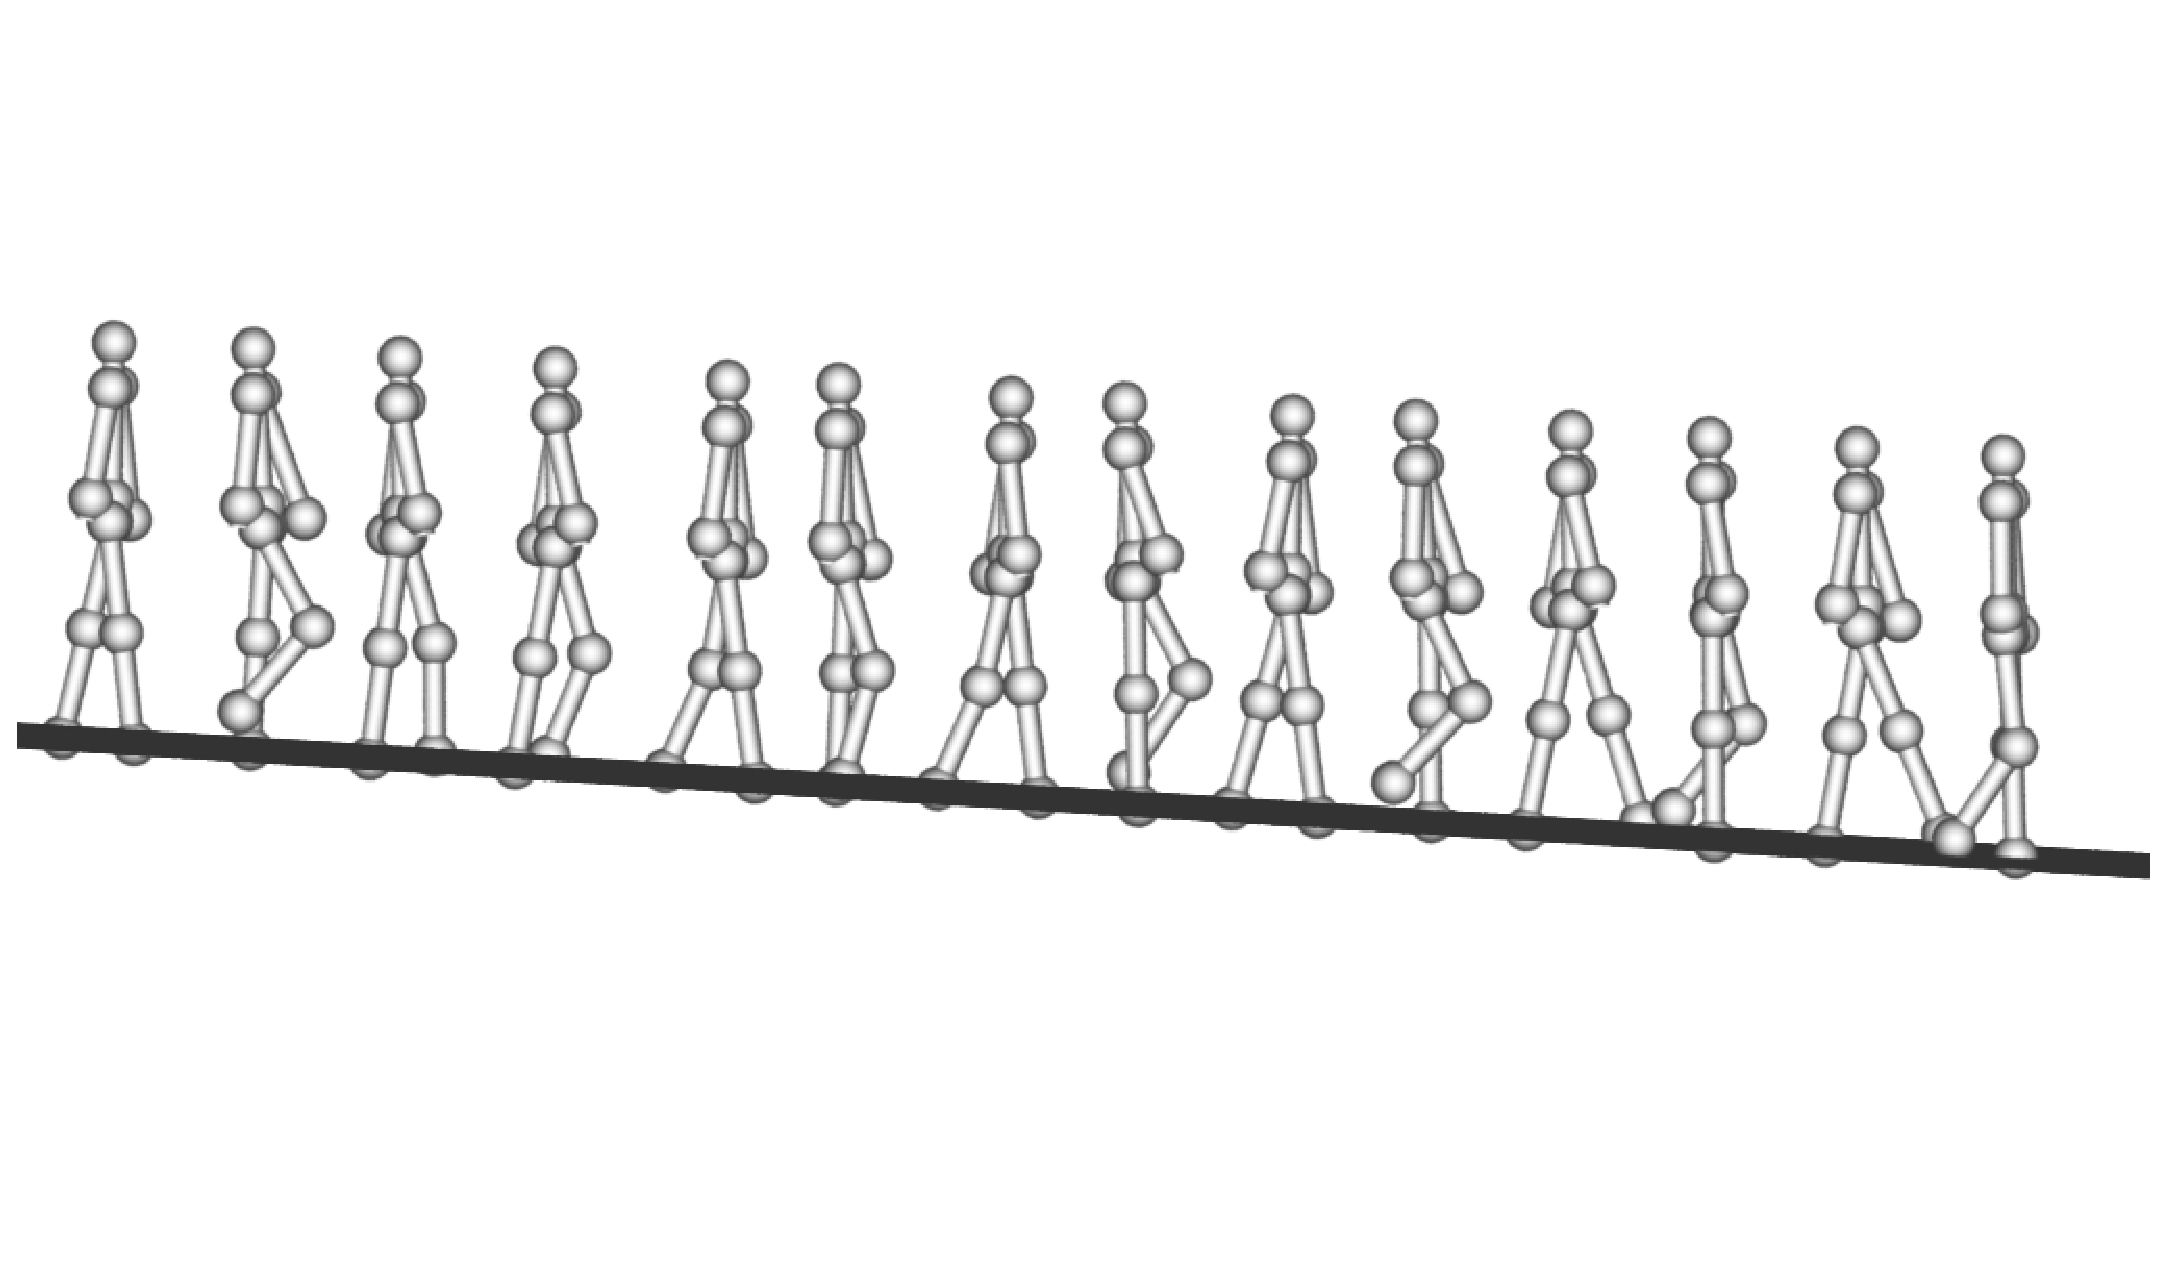
\includegraphics[width=0.7\textwidth]{smallStep}
    \caption{Small Initial Step Size}
    \label{fig:smallStepini}
\end{center}
\end{figure}


\begin{figure}[!htbp]
  \begin{center}
      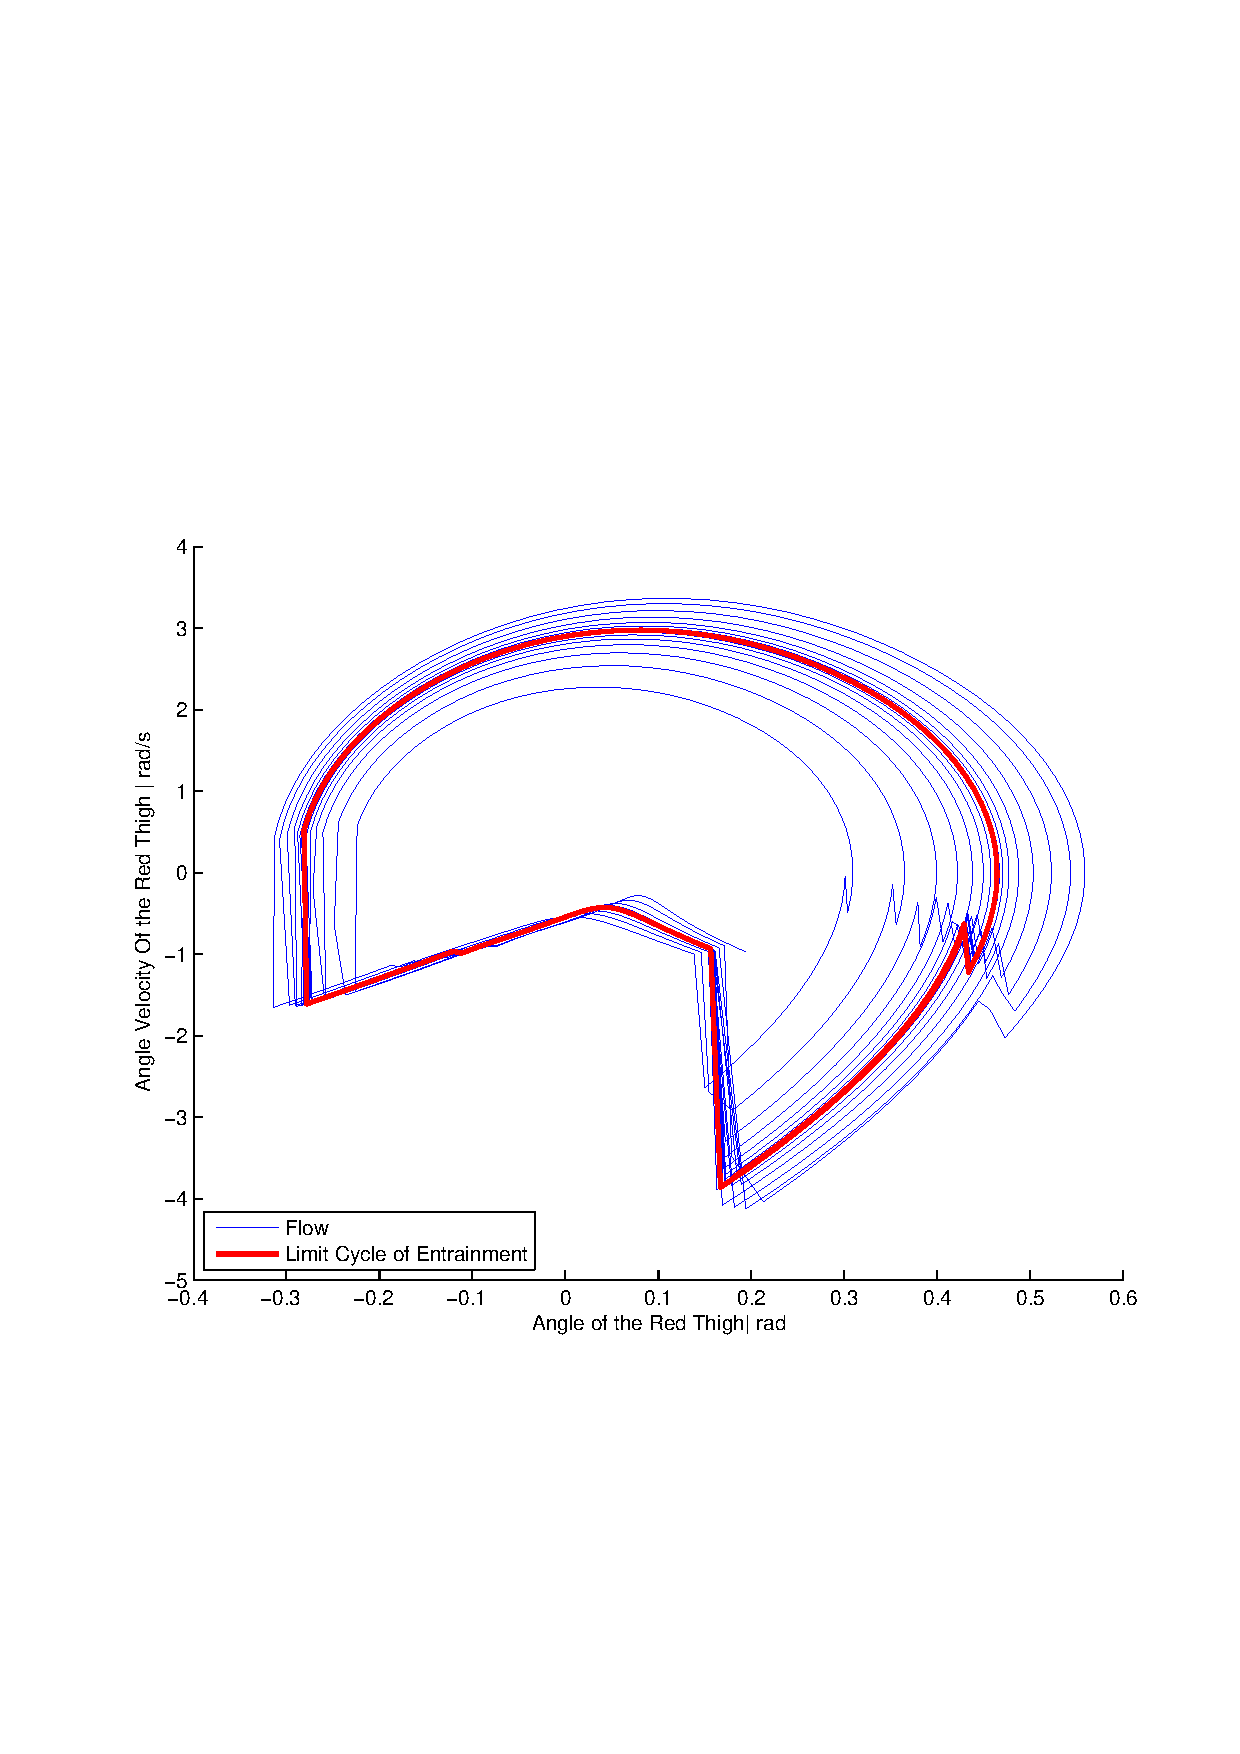
\includegraphics[width=0.7\textwidth]{BigStepPhasePlot}
    \caption{Big Initial Step Initial Phase Plot}
    \label{fig:bigstepiniGaitPlot}
\end{center}
\end{figure}


\begin{figure}[!htbp]
  \begin{center}
      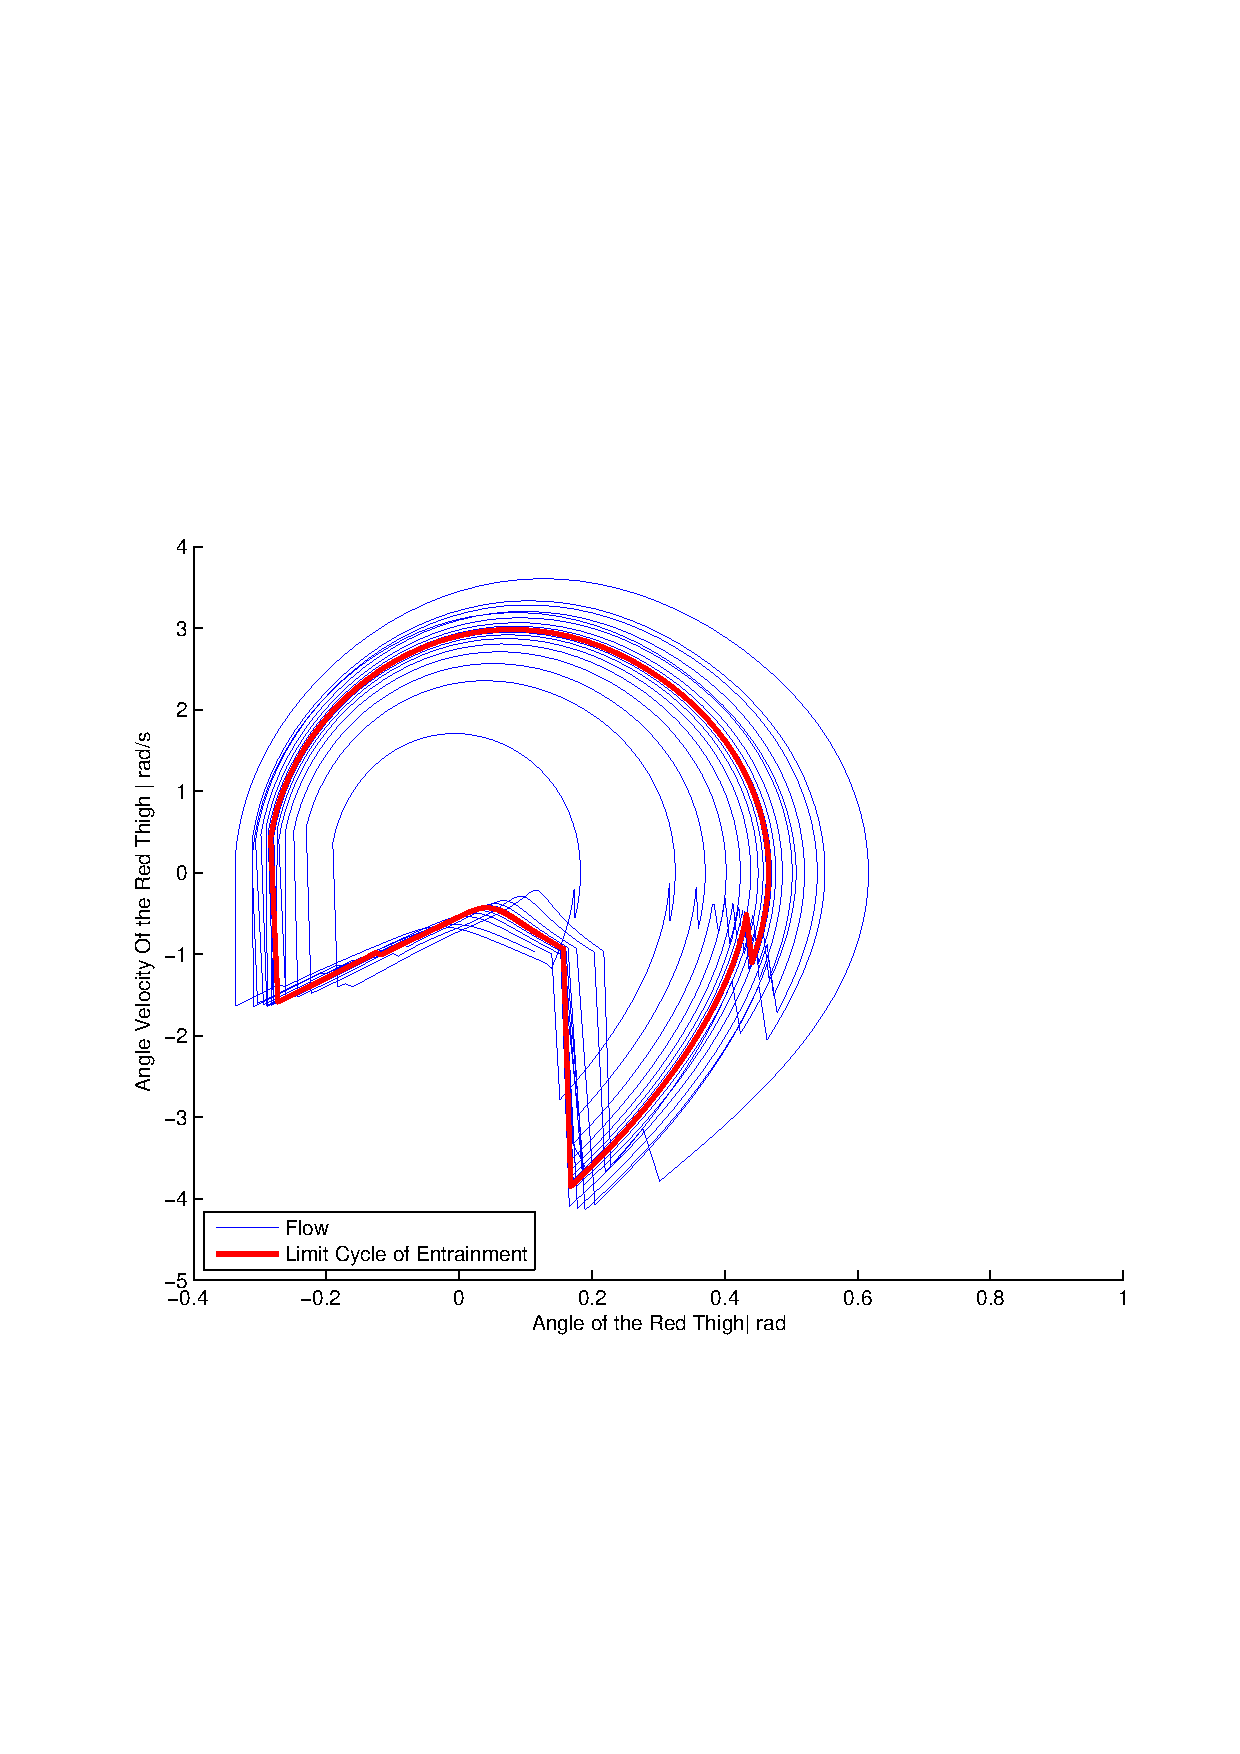
\includegraphics[width=0.7\textwidth]{SmallStepPhasePlot}
    \caption{The Small Initial Step Gait Phase Plot}
    \label{fig:smallstepiniPhasePlot}
\end{center}
\end{figure}







\subsection{System Gait Adaptation}
The passive walker has many parameters, like mass and leg length, different parameters will result in a different dynamics sytem.
But all these dynamic systems  share the same topology and generate different limit cycle and gaits.
Some meaningful gaits are shown.

If all the parameters are scaled in uniform, the gait will remain the same, only the velocity will be changed,
To demonstrate different gaits, ratio parameters are modified. 
The total mass and total leg length of all examples are kept the same.



\subsubsection*{Mass Distribution Ratio}
When the total mass is kept,
Mass Distribution Ratio is defined as the hip mass over leg mass. 
The mass ratios of shank and thigh are kept.
thus we define the ratio as
\[
\alpha_m=\frac{m_h}{m_s}
\]
where $m_h$ is the mass of the hip and $m_t$ is mass of the thigh.
Different $\alpha_m$ will result in different gait, bigger $\alpha_m$ result gait to that burdened.
Different limit cycles are shown in Figure ~\ref{fig:differentmh}.
\begin{figure}[!htbp]
  \begin{center}
     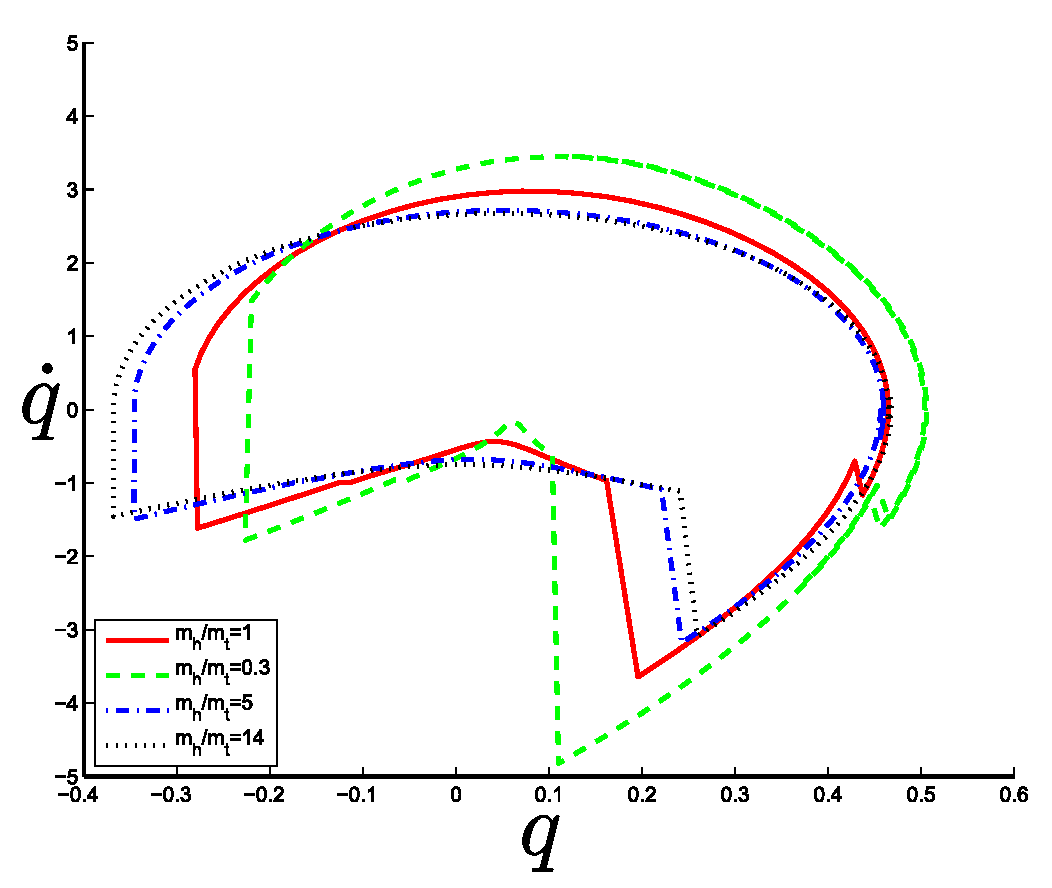
\includegraphics[width=0.7\textwidth]{MassDistributionEffectsOnLimitCircle}
    \caption{Different Gait Resulting From the Different Mass Ratio}
    \label{fig:differentmh}
\end{center}
\end{figure}

For bigger $\alpha_m$, the walker will walk with bigger step but a slow speed($\qd$ is lower).
Also the character tend to fall backward.
For smaller $\alpha_m$, character will walk with quickly($\qd$ is bigger) and it tends to lean forward.
This may imply about the upper body motion.
Usually, when we carry something heavier, we  tend to bend upperbody forward.

Different gaits are shown in Figure~\ref{fig:massh1},Figure~\ref{fig:massh2},Figure~\ref{fig:massh3}
\begin{figure}[!htbp]
  \begin{center}
      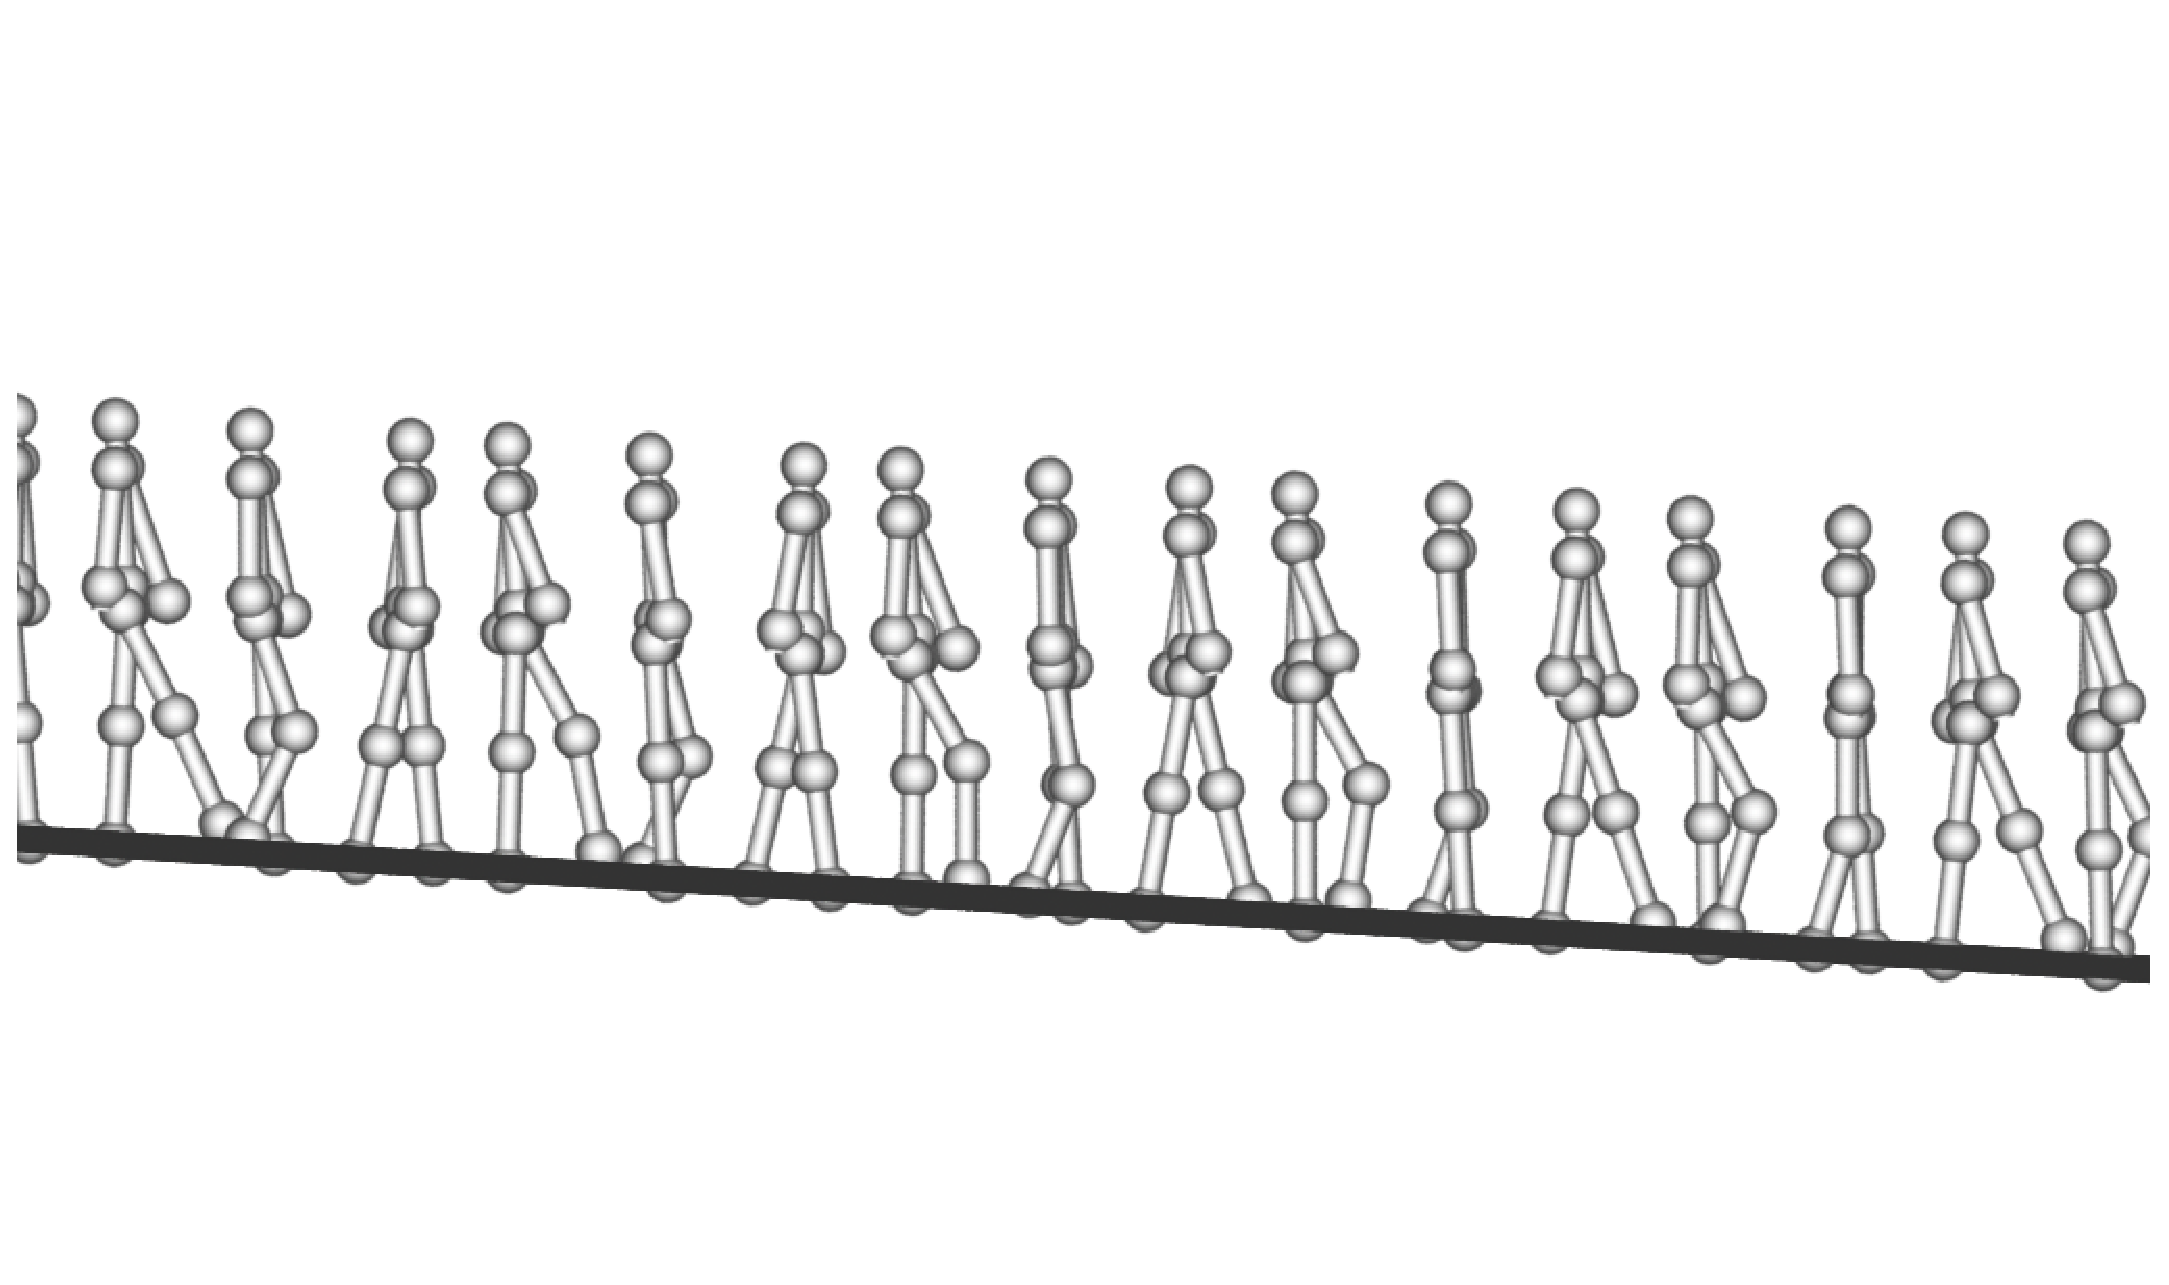
\includegraphics[width=0.7\textwidth]{mhms3}
    \caption{gait with $\alpha_m=0.3$}
    \label{fig:massh1}
\end{center}
\end{figure}

\begin{figure}[!htbp]
  \begin{center}
      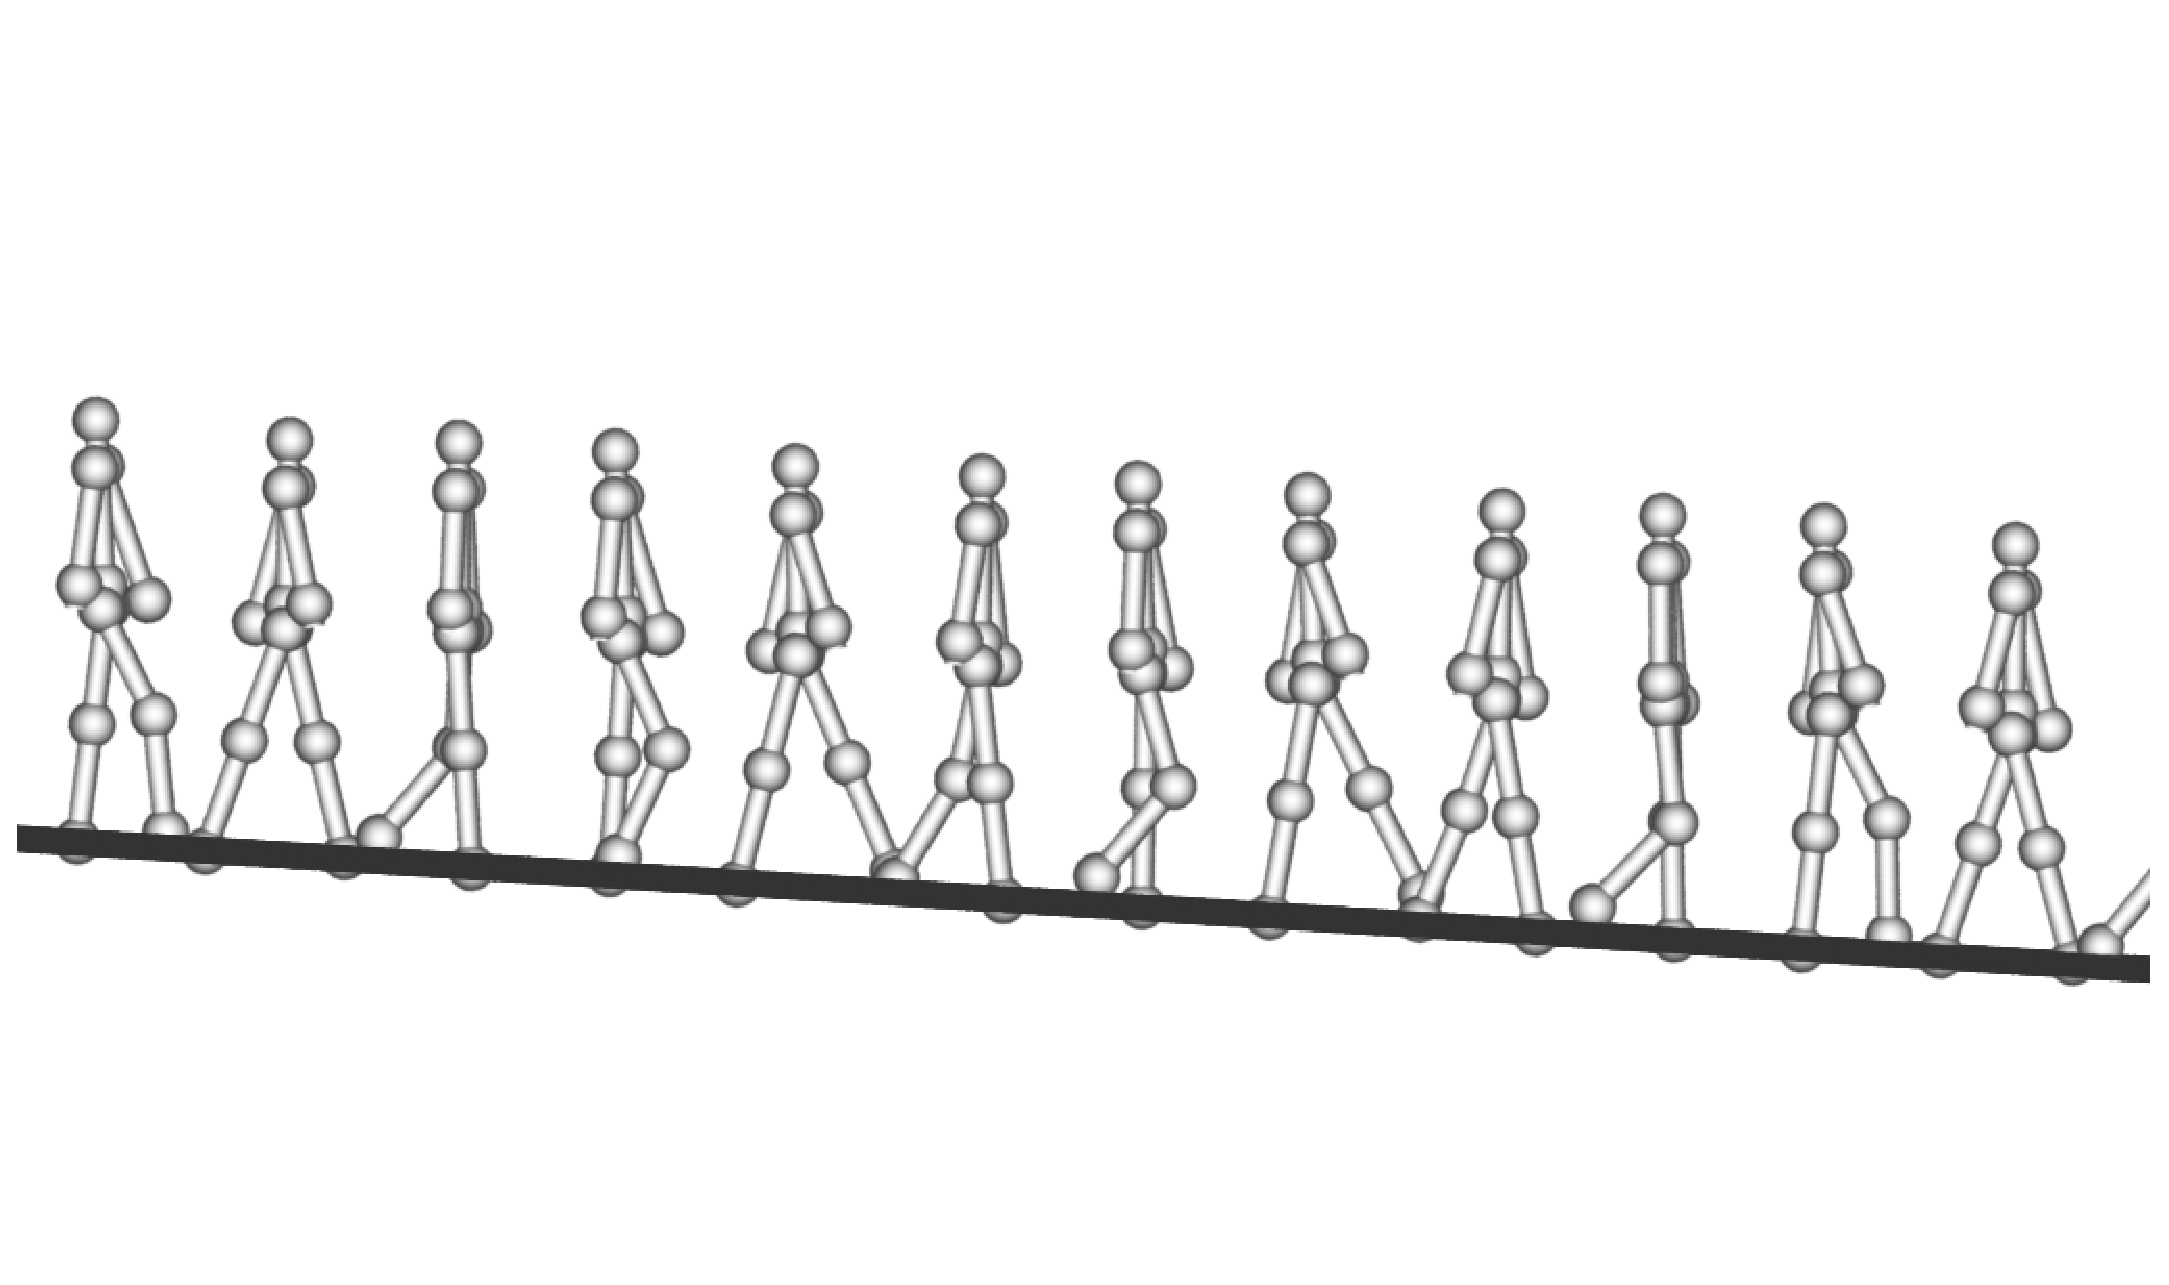
\includegraphics[width=0.7\textwidth]{mhms50}
    \caption{Gait of $\alpha_m=5$}
    \label{fig:massh2}
\end{center}
\end{figure}

\begin{figure}[!htbp]
  \begin{center}
      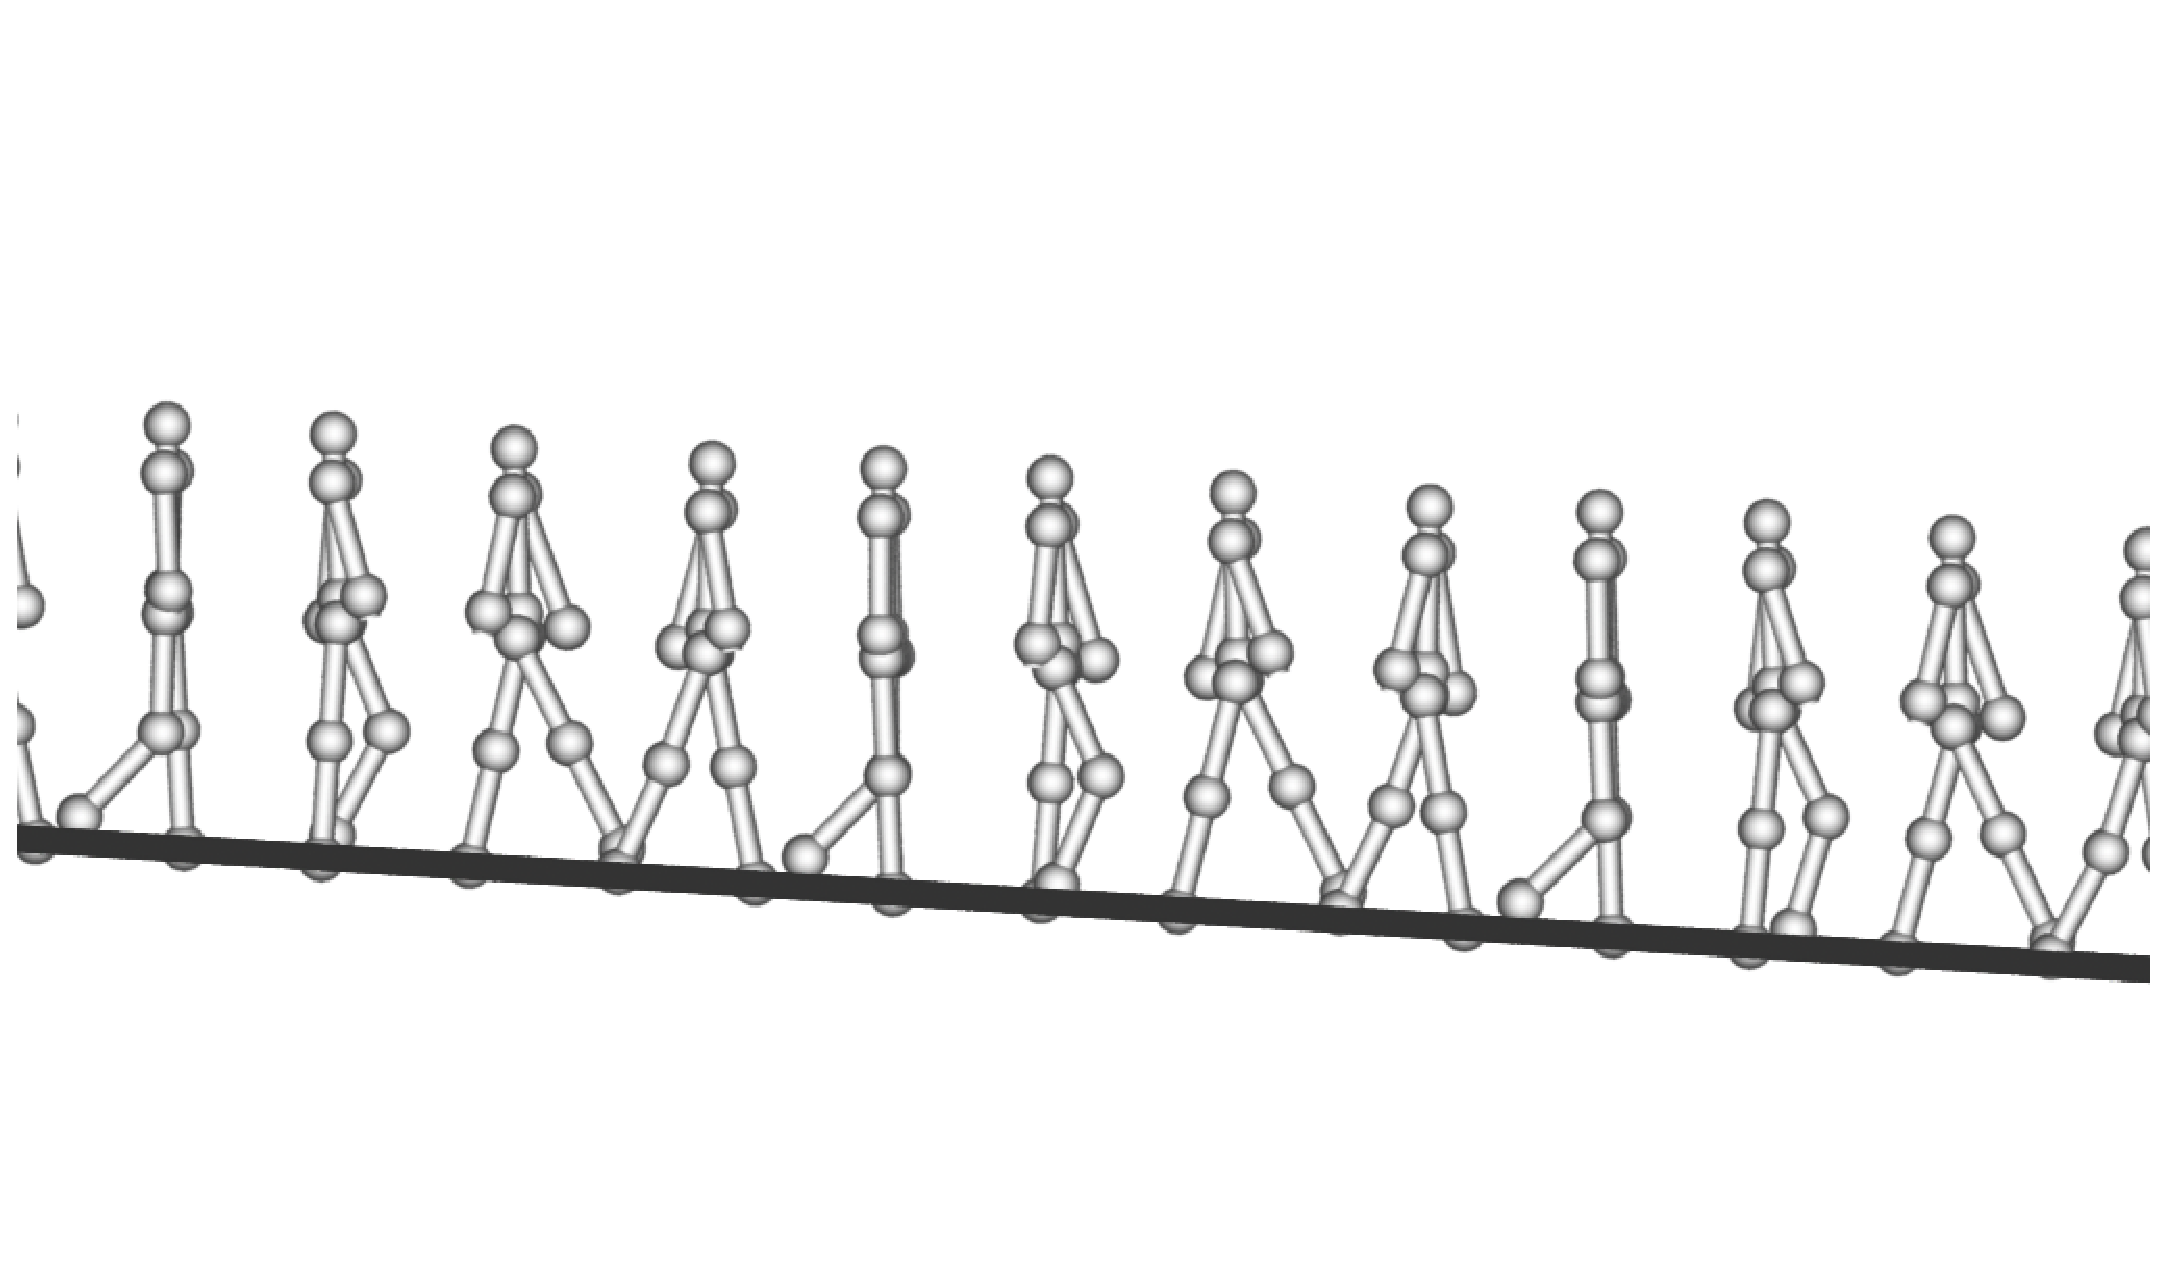
\includegraphics[width=0.7\textwidth]{mhms140}
    \caption{Gait of $\alpha_m=14$}
    \label{fig:massh3}
\end{center}
\end{figure}



\subsubsection*{Leg Length Distribution Ratio}
The leg length is kept unchanged, but we alter the the ration parameter $\alpha_l=\frac{l_t}{l_s}$.
By chaning $\alpha_l$ motion for different characters are generated.
This demostrated the motion retargeting resullts.


\begin{figure}[!htbp]
  \begin{center}
      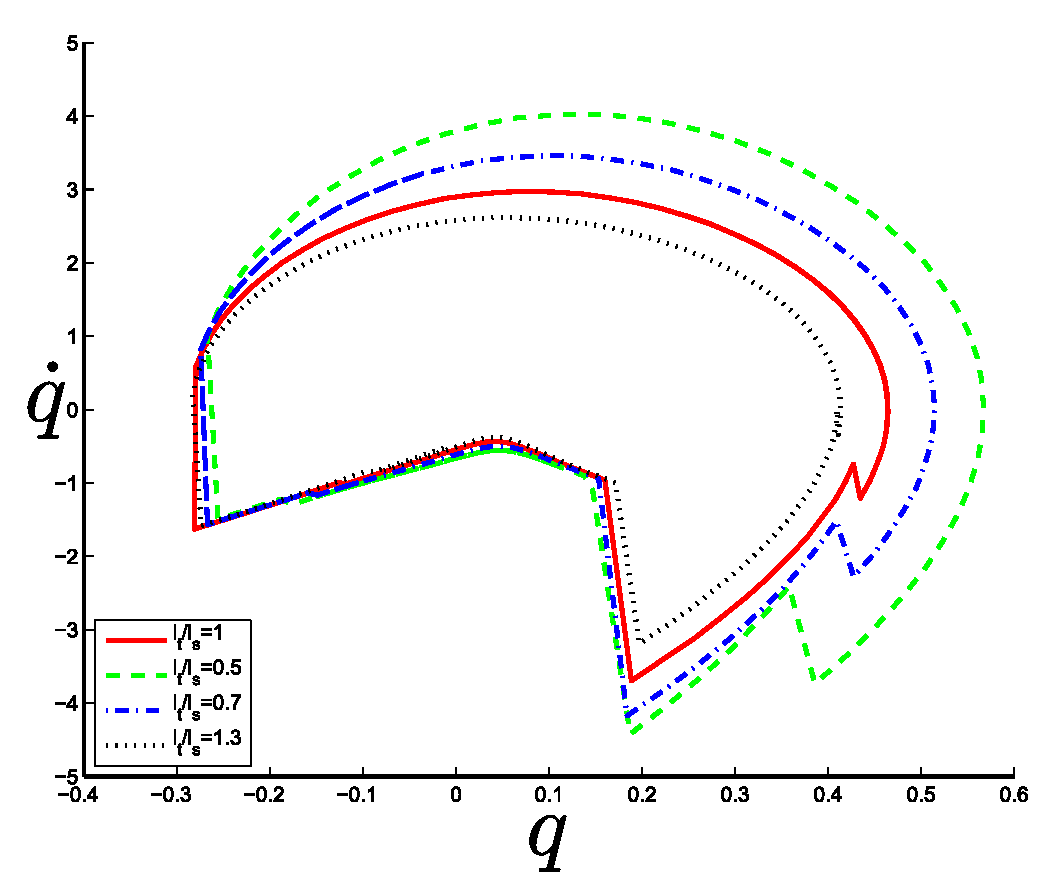
\includegraphics[width=0.7\textwidth]{LegLengthDistributionEffectsOnLimitCircle}
    \caption{Different Gait Resulting From the Different Mass Ratio}
    \label{fig:differentlr}
\end{center}
\end{figure}

The limit cycle in Figure~\ref{fig:differentlr} imply something important about leg length in walking.
Basically, the support leg motion is almost the same, while different leg length ration will result in different sway angle
The step size is kept.
The longer the shank, thigh has to sway quickly and with bigger amplitude.
There are also bigger impulses during the strike phase. 
For both the knee and heel strike, larger impulse is generated.
This result may shows the effects of high heel shoes for walking.
Figure~\ref{fig:lr1},Figure~\ref{fig:lr2},Figure~\ref{fig:lr3} show the different gaits.



\begin{figure}[!htbp]
  \begin{center}
      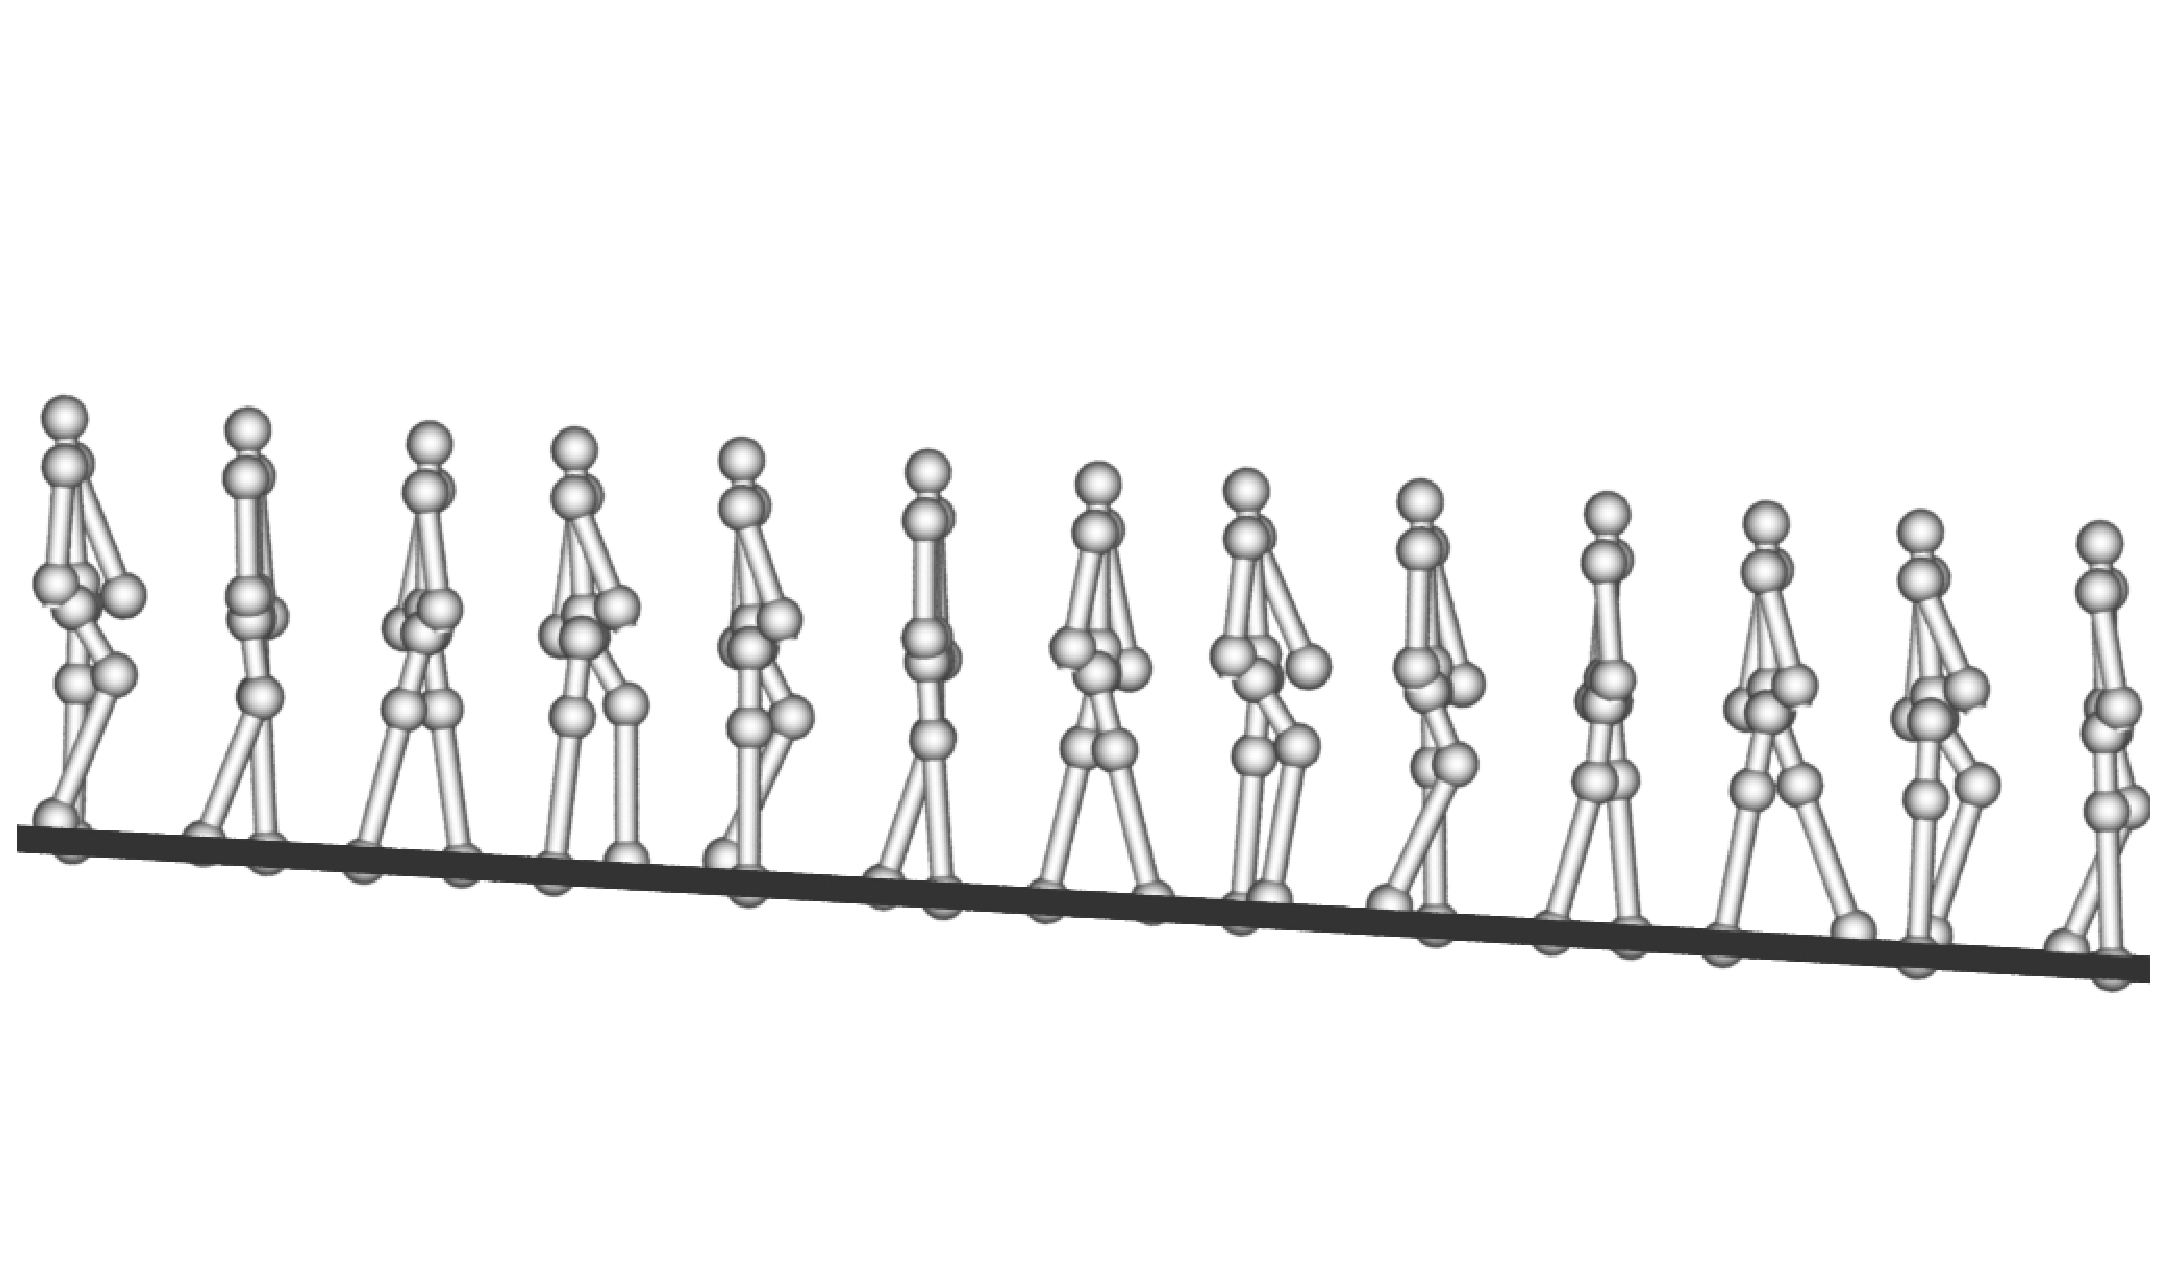
\includegraphics[width=0.7\textwidth]{LTLS5}
    \caption{gait of $\alpha_l=0.5$}
    \label{fig:lr1}
\end{center}
\end{figure}

\begin{figure}[!htbp]
  \begin{center}
      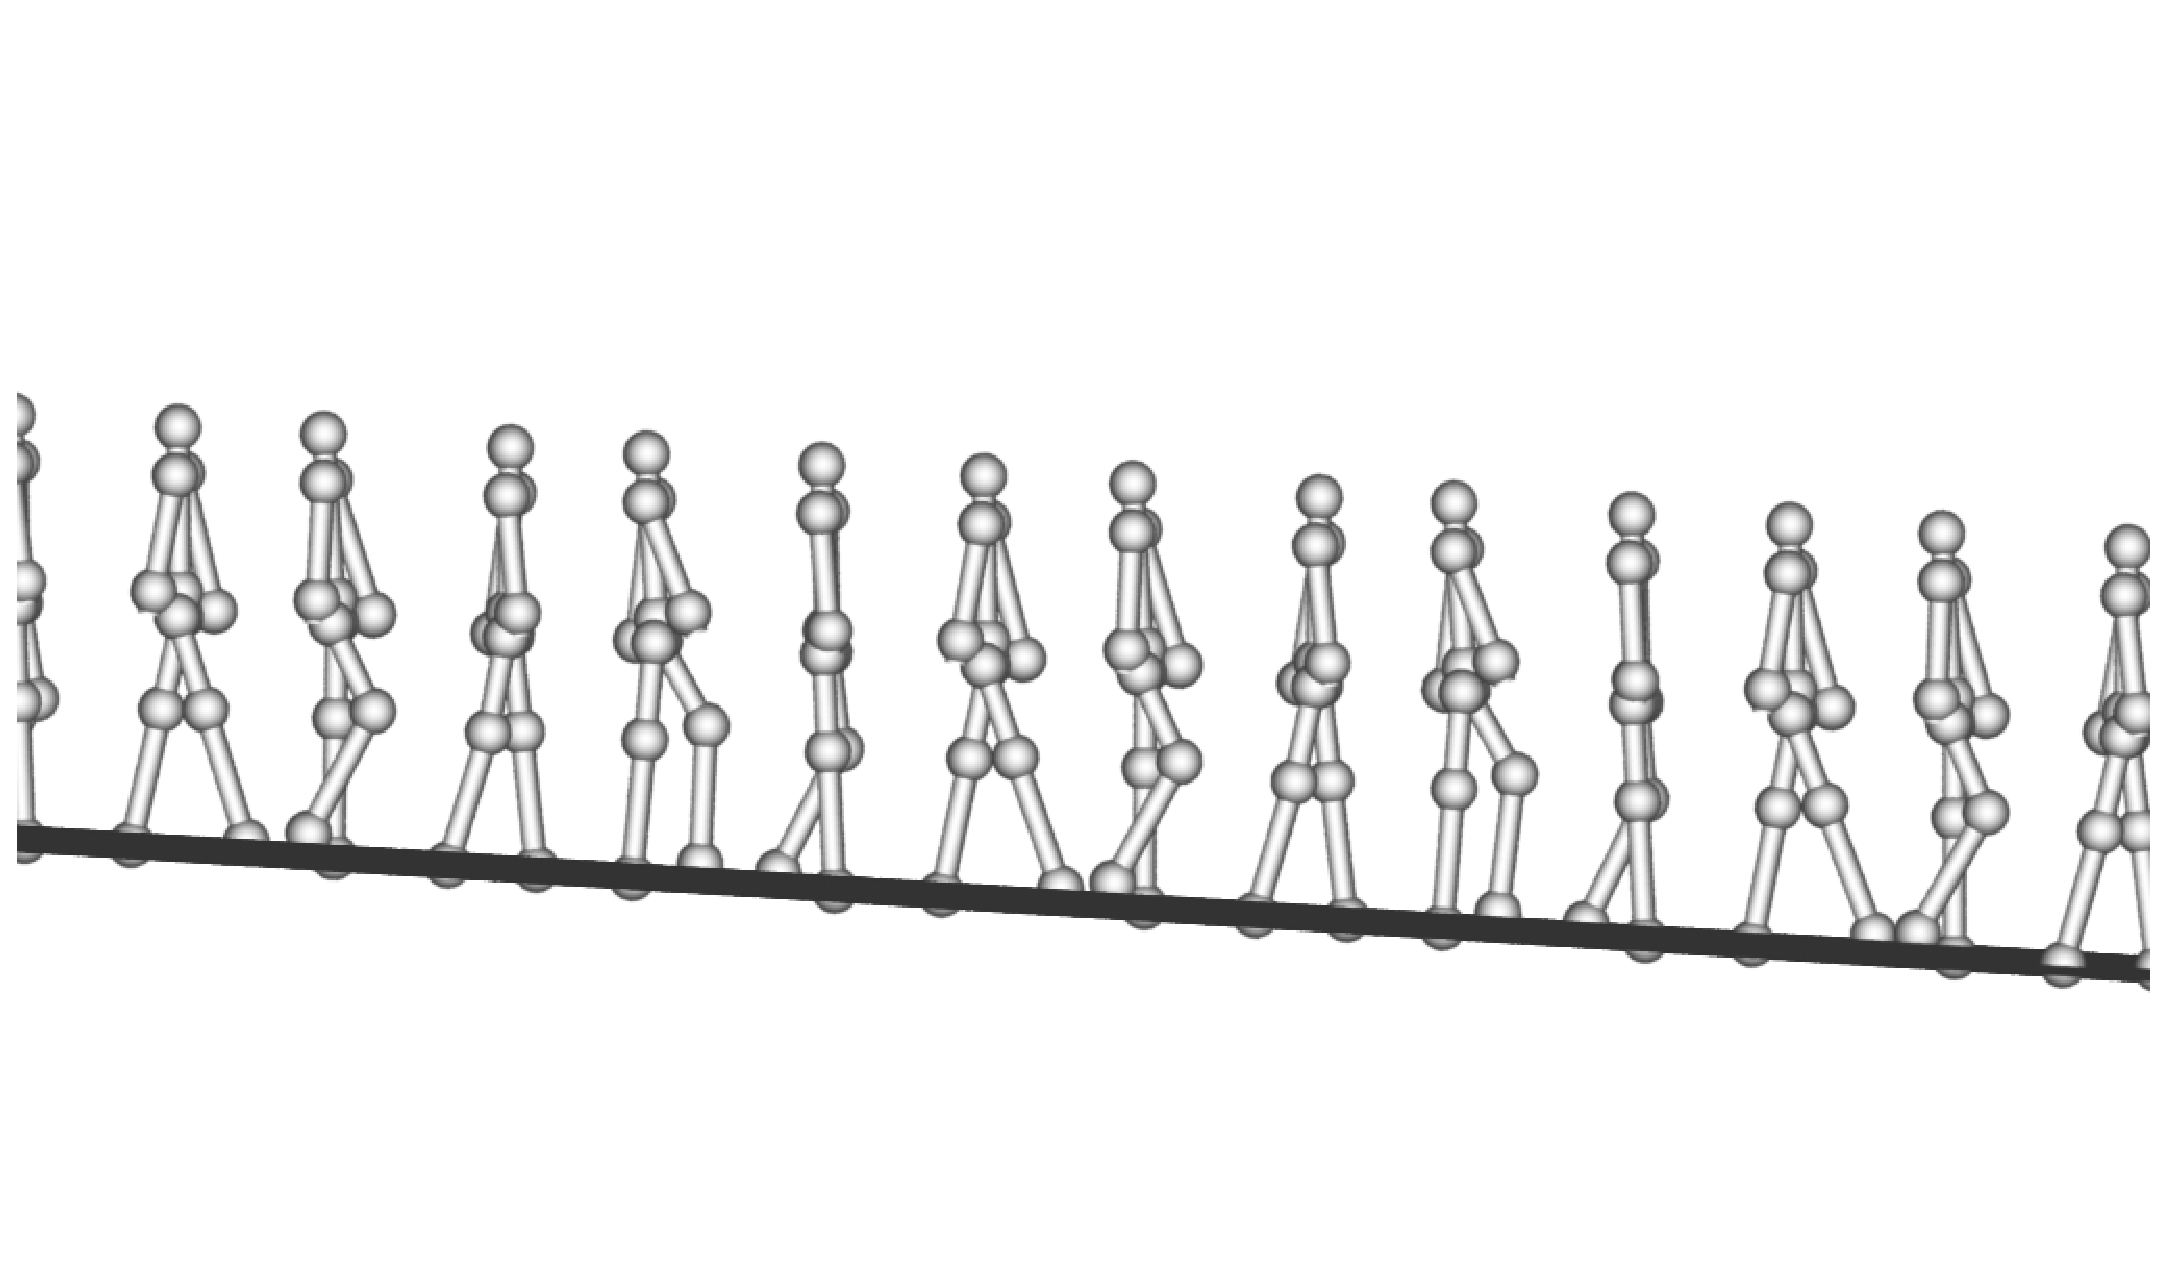
\includegraphics[width=0.7\textwidth]{LTLS7}
    \caption{gait of $\alpha_l=0.7$}
    \label{fig:lr2}
\end{center}
\end{figure}

\begin{figure}[!htbp]
  \begin{center}
      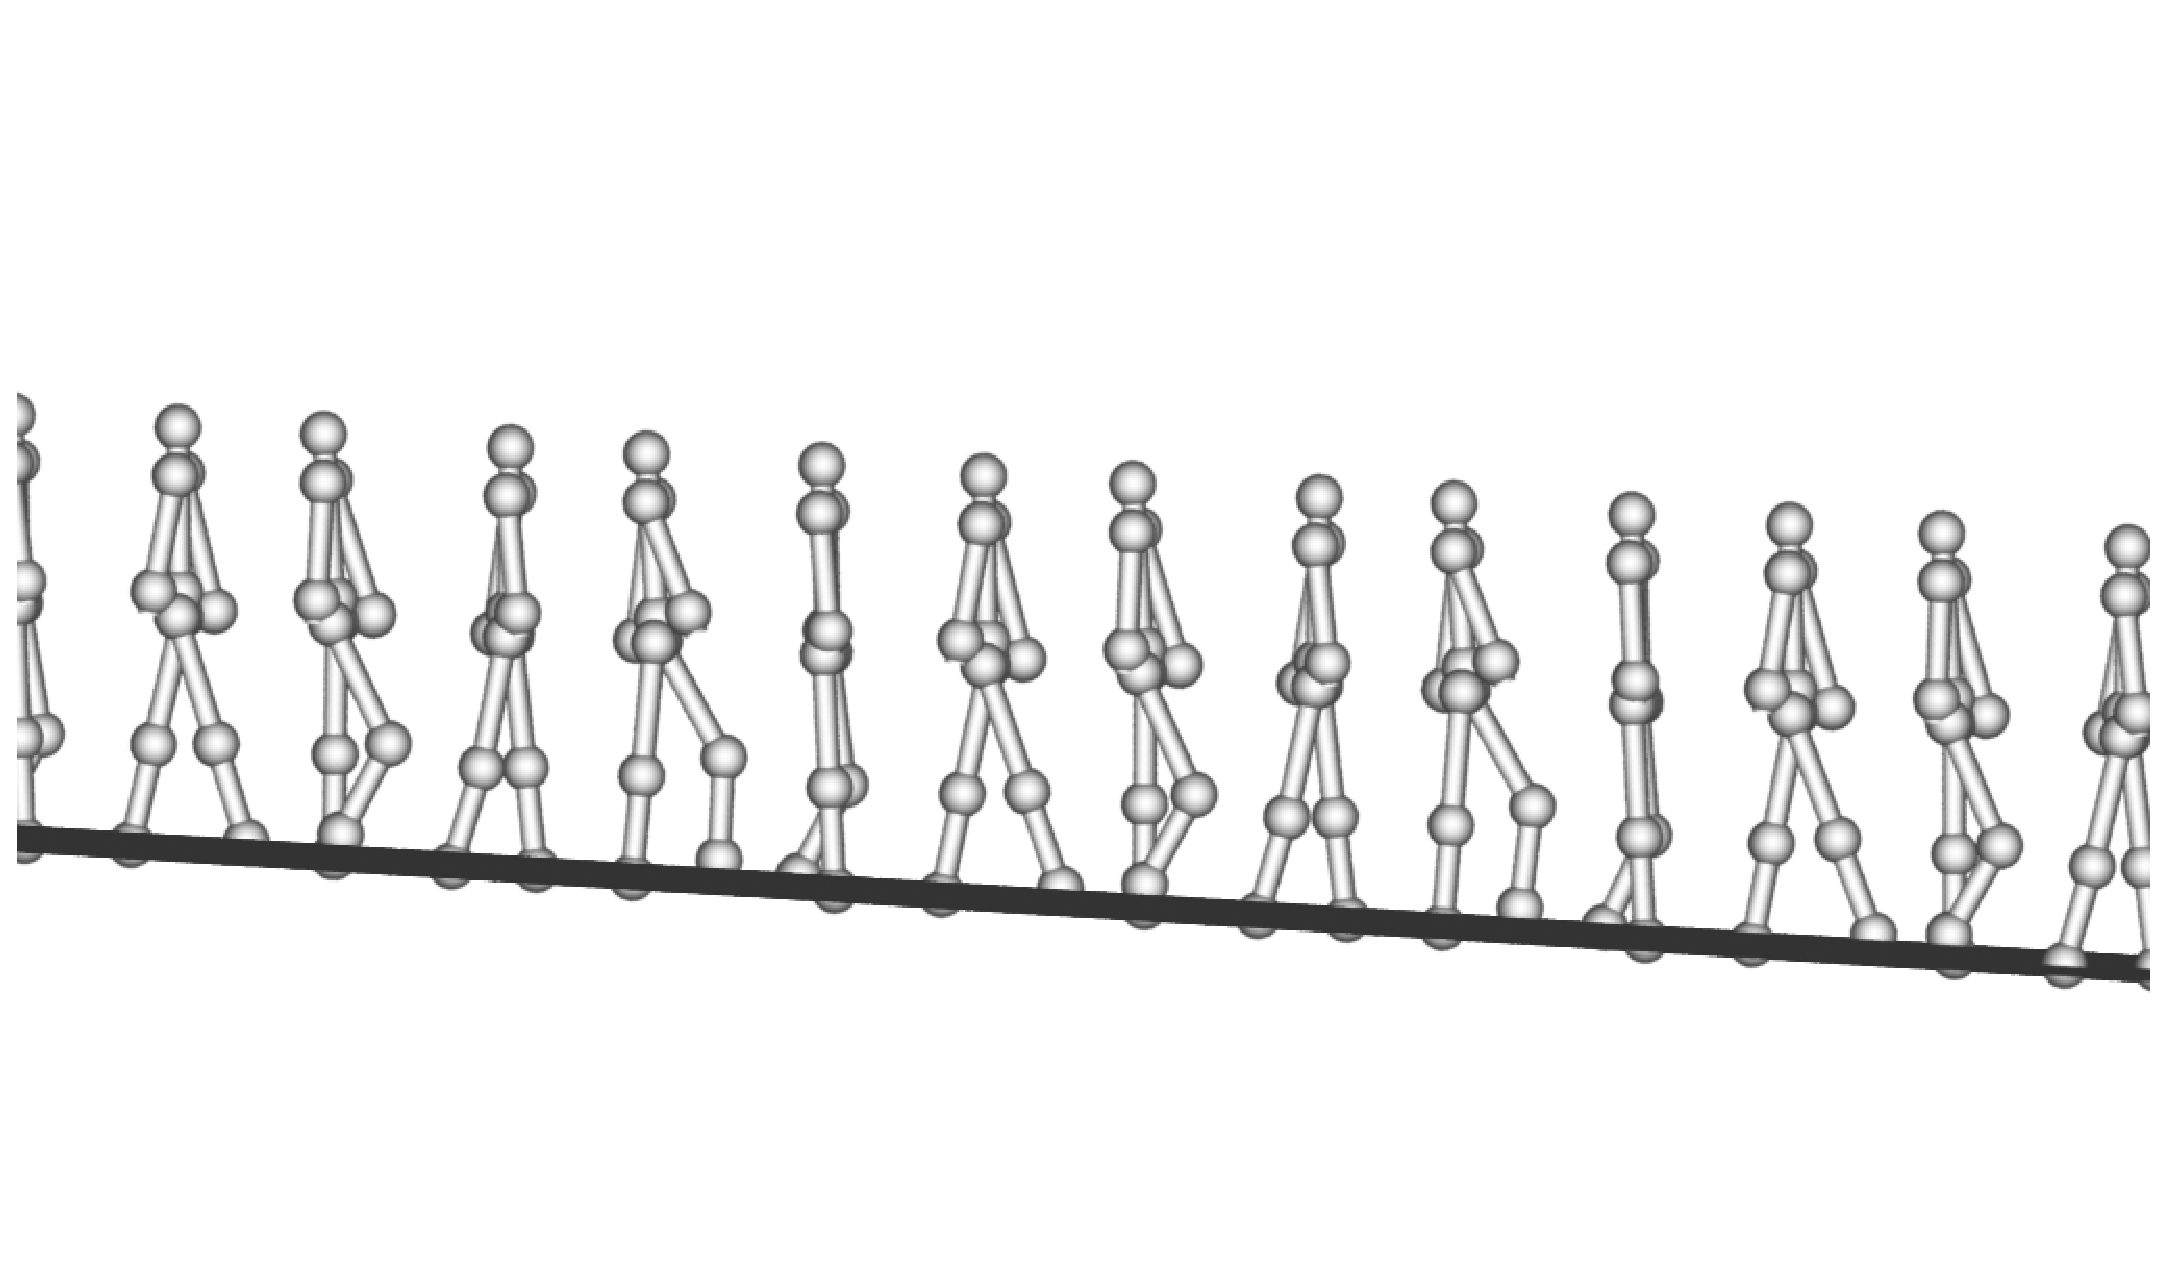
\includegraphics[width=0.7\textwidth]{LTLS13}
    \caption{gait of $\alpha_l=1.3$}
    \label{fig:lr3}
\end{center}
\end{figure}





\subsubsection*{Unbalanced Mass Ratio}
Also define the \emph{Unbalanced Mass Ration} $\alpha_b=\frac{\text{Left Leg Mass}}{\text{Right Leg Mass}}$.
When $\alpha_b$ is increased, two legs sway differently and the limit circle is splited.
Bigger $\alpha_b$  will result in cripple like gait, as shown in Figure~\ref{fig:lm2}

\begin{figure}[!htbp]
  \begin{center}
      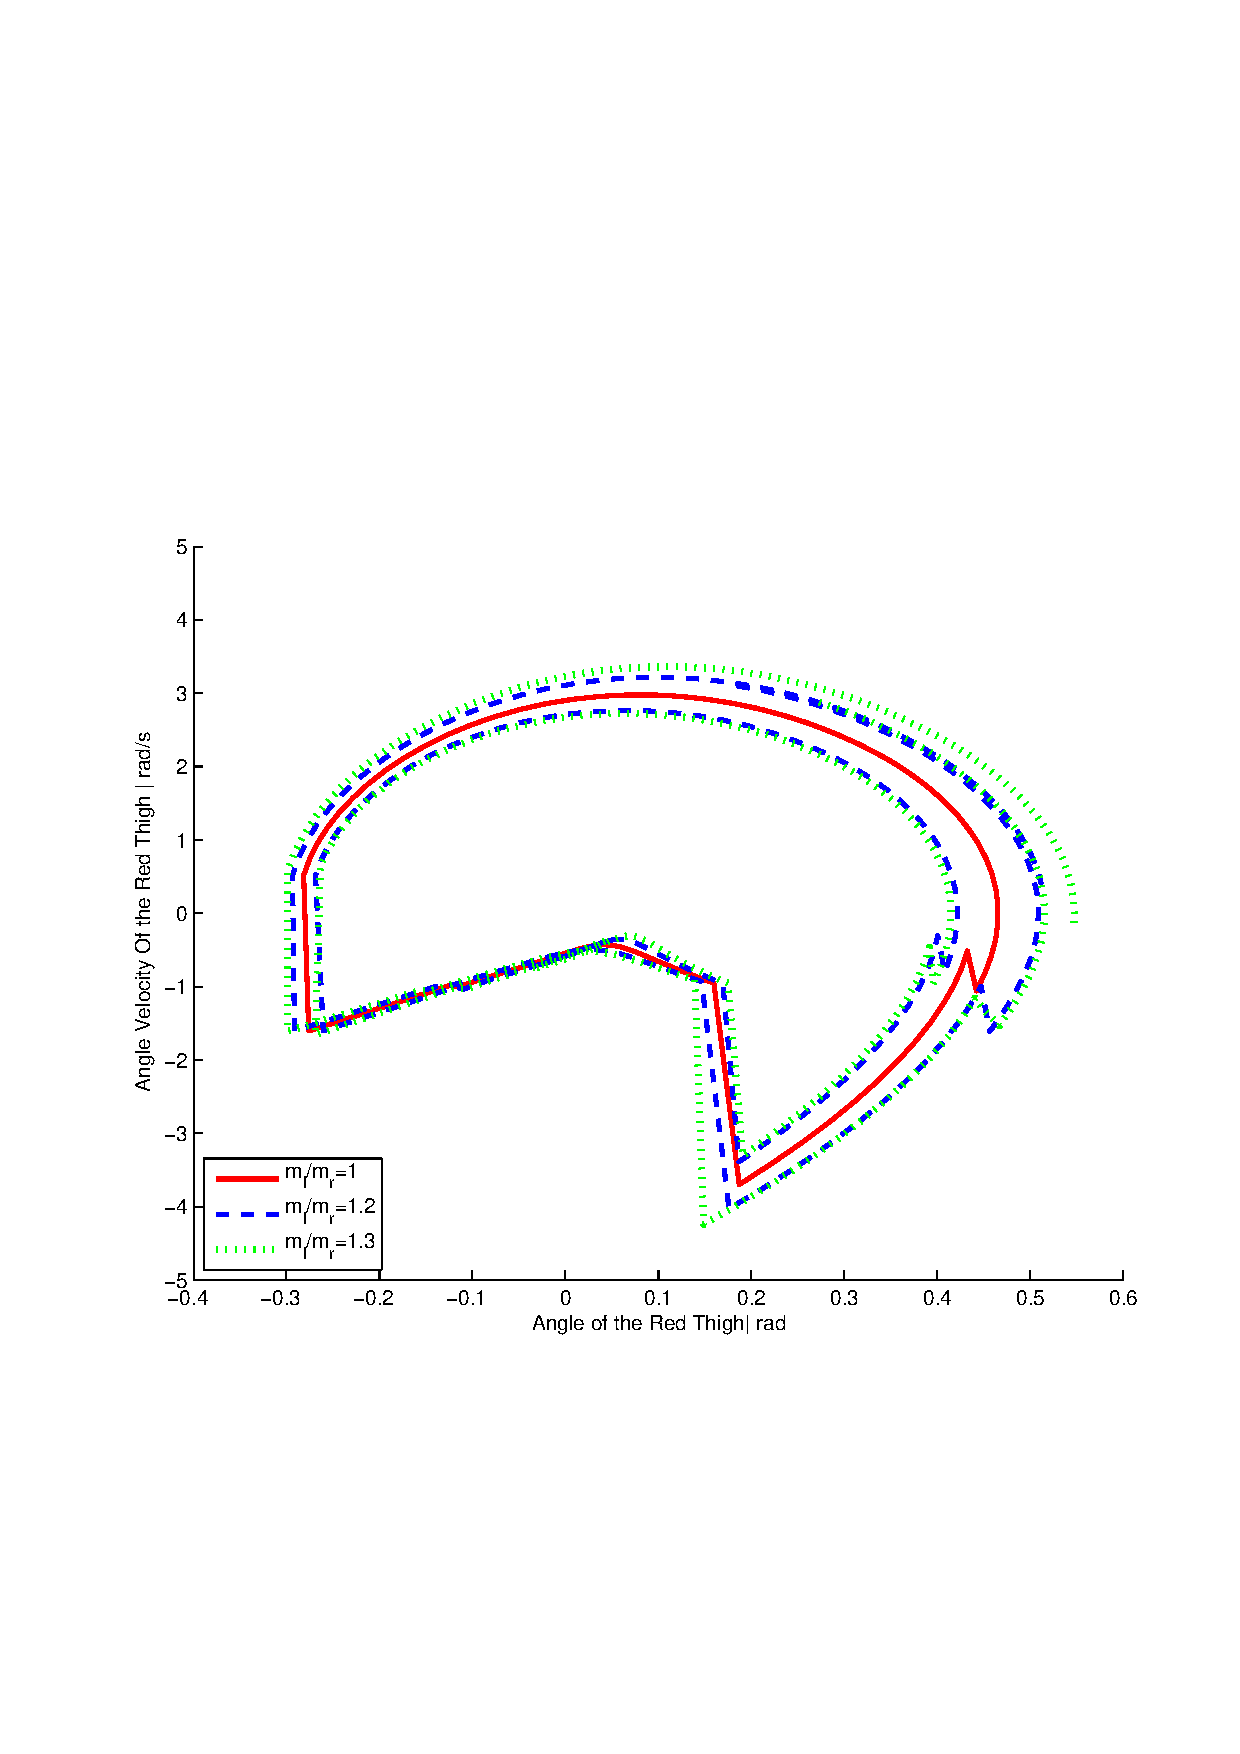
\includegraphics[width=0.7\textwidth]{DifferentLegMassLimitCircle}
    \caption{Different Leg Mass Stable Gaits}
    \label{fig:differentlr}
\end{center}
\end{figure}




\begin{figure}[!htbp]
  \begin{center}
      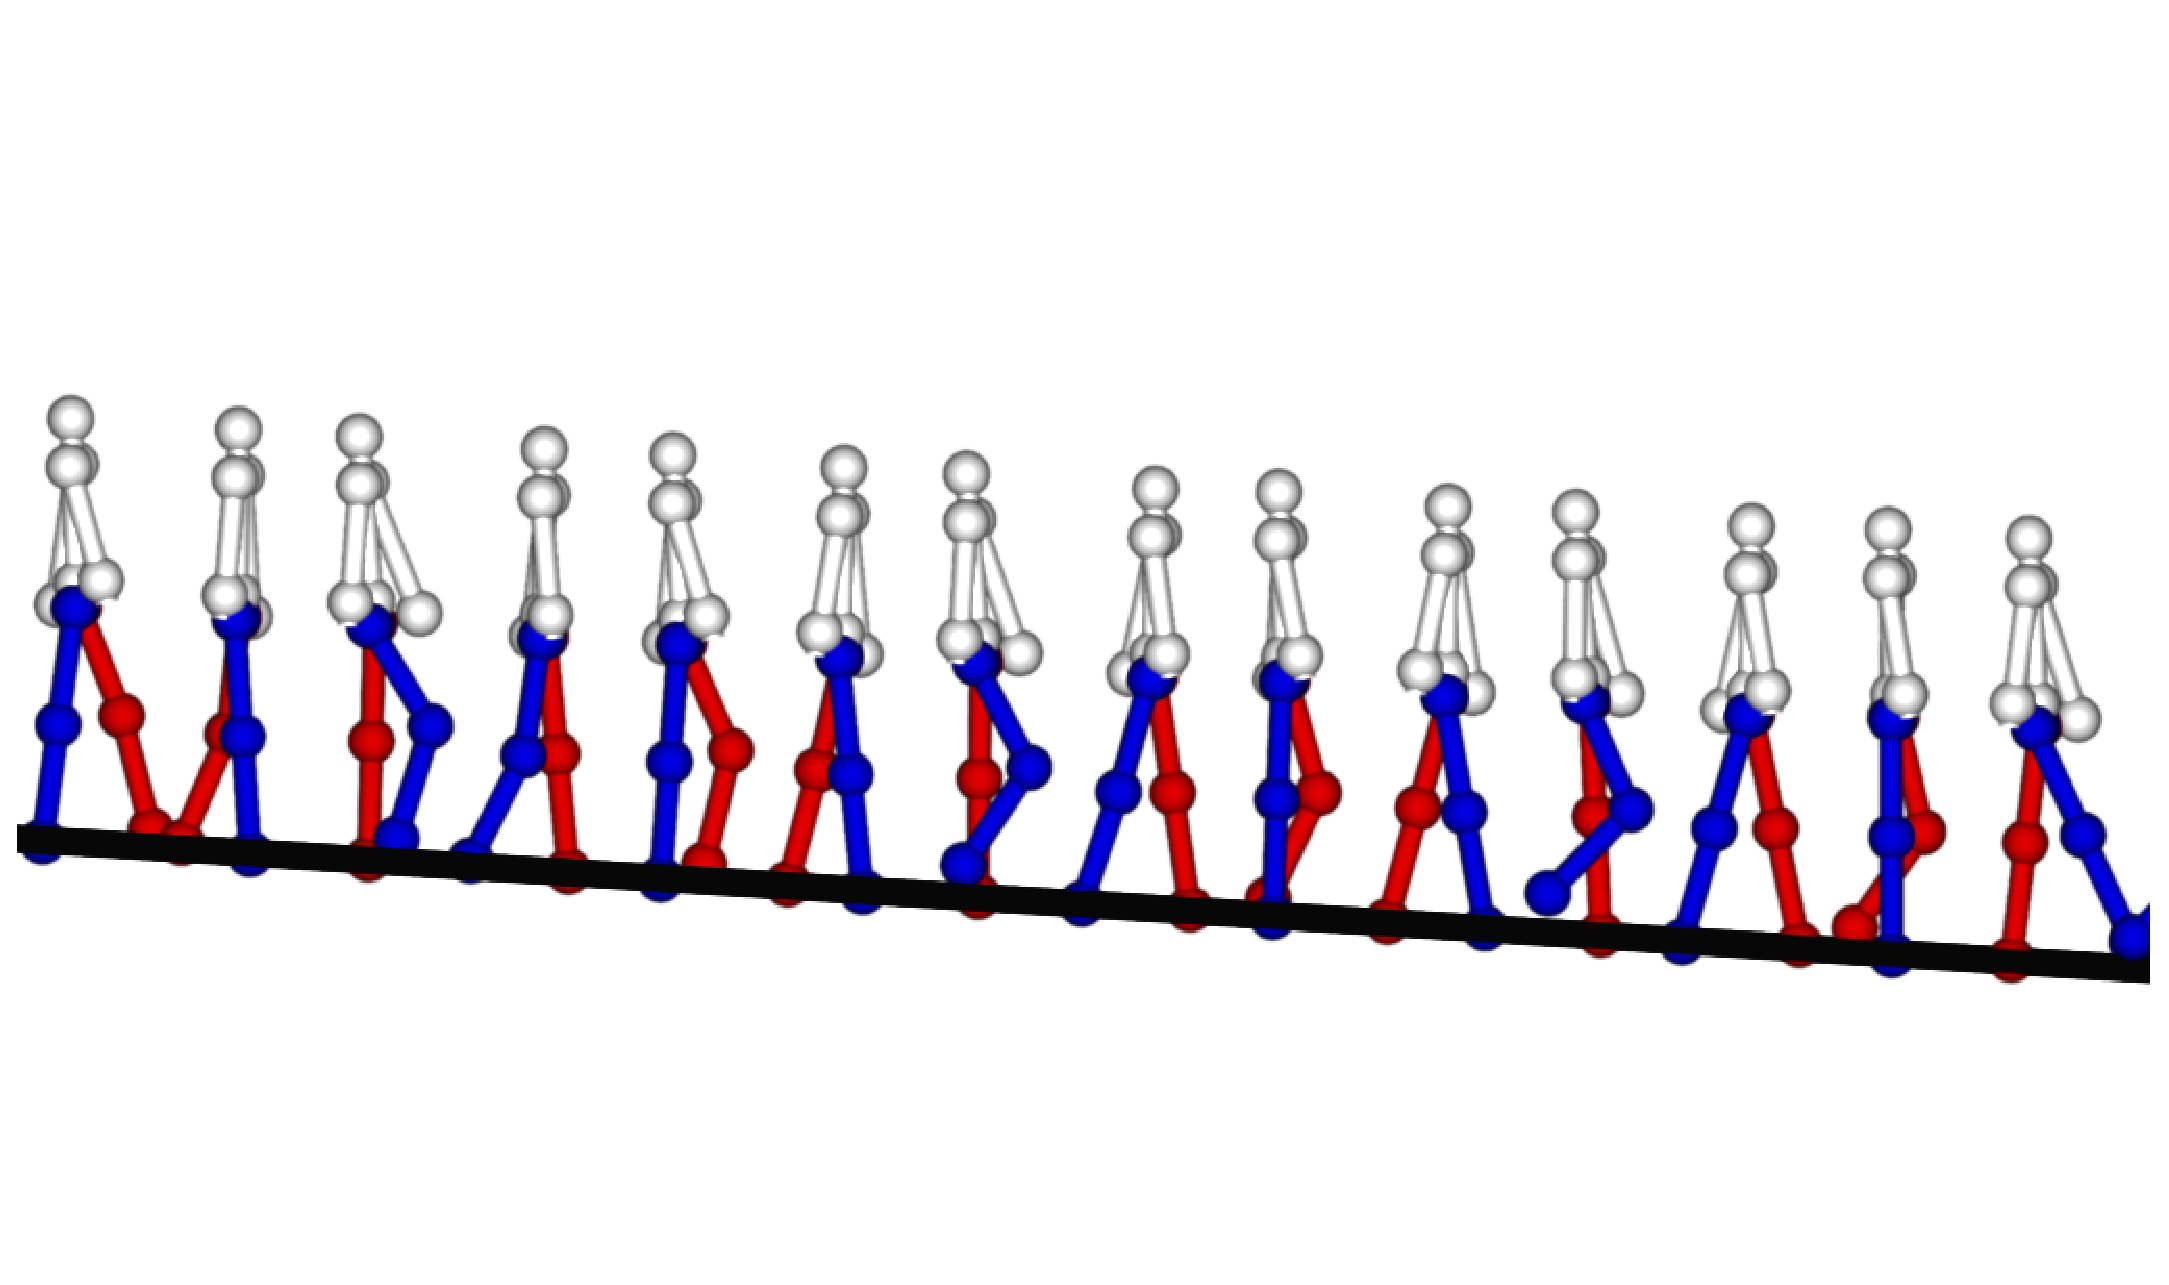
\includegraphics[width=0.7\textwidth]{MLMR130}
    \caption{Gait of $\alpha_b=1.3$}
    \label{fig:lm2}
\end{center}
\end{figure}



\subsubsection*{Different Slopes}
Also we can change the angle of downslope.
For different slopes, entrainment maintains the limit cycle, but limit cycle changed its shape.
Different stable limit cycles are show in Figure ~\ref{fig:diffslopes}
Basically, the bigger the slope, the bigger the step size, the higher the speed.
Slope changing has similar effects to energy scaling.
Figure~\ref{fig:ss1},Figure~\ref{fig:ss2},Figure~\ref{fig:ss3} shown different gaits on different slopes.


\begin{figure}[!htbp]
  \begin{center}
      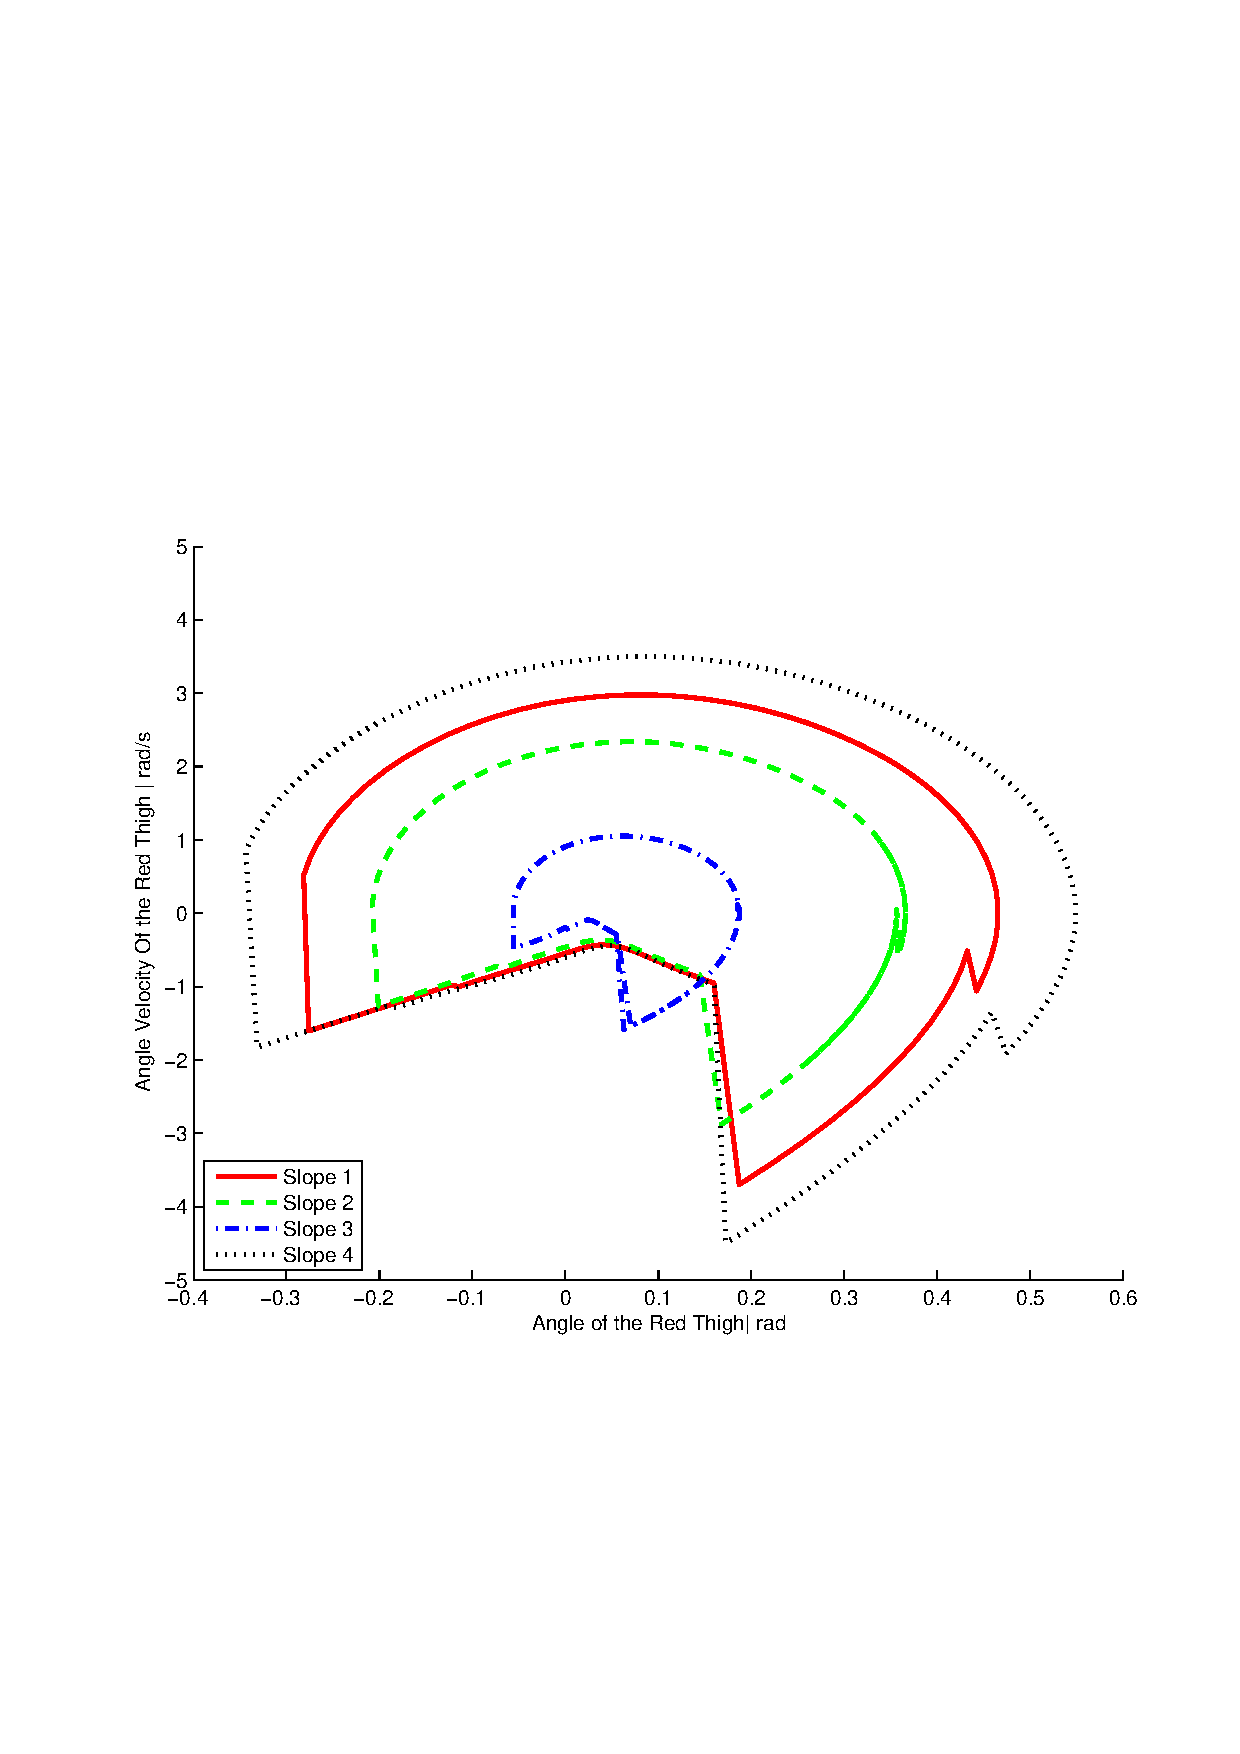
\includegraphics[width=0.7\textwidth]{DifferentSlope}
    \caption{different step size walking}
    \label{fig:diffslopes}
\end{center}
\end{figure}


\begin{figure}[!htbp]
  \begin{center}
      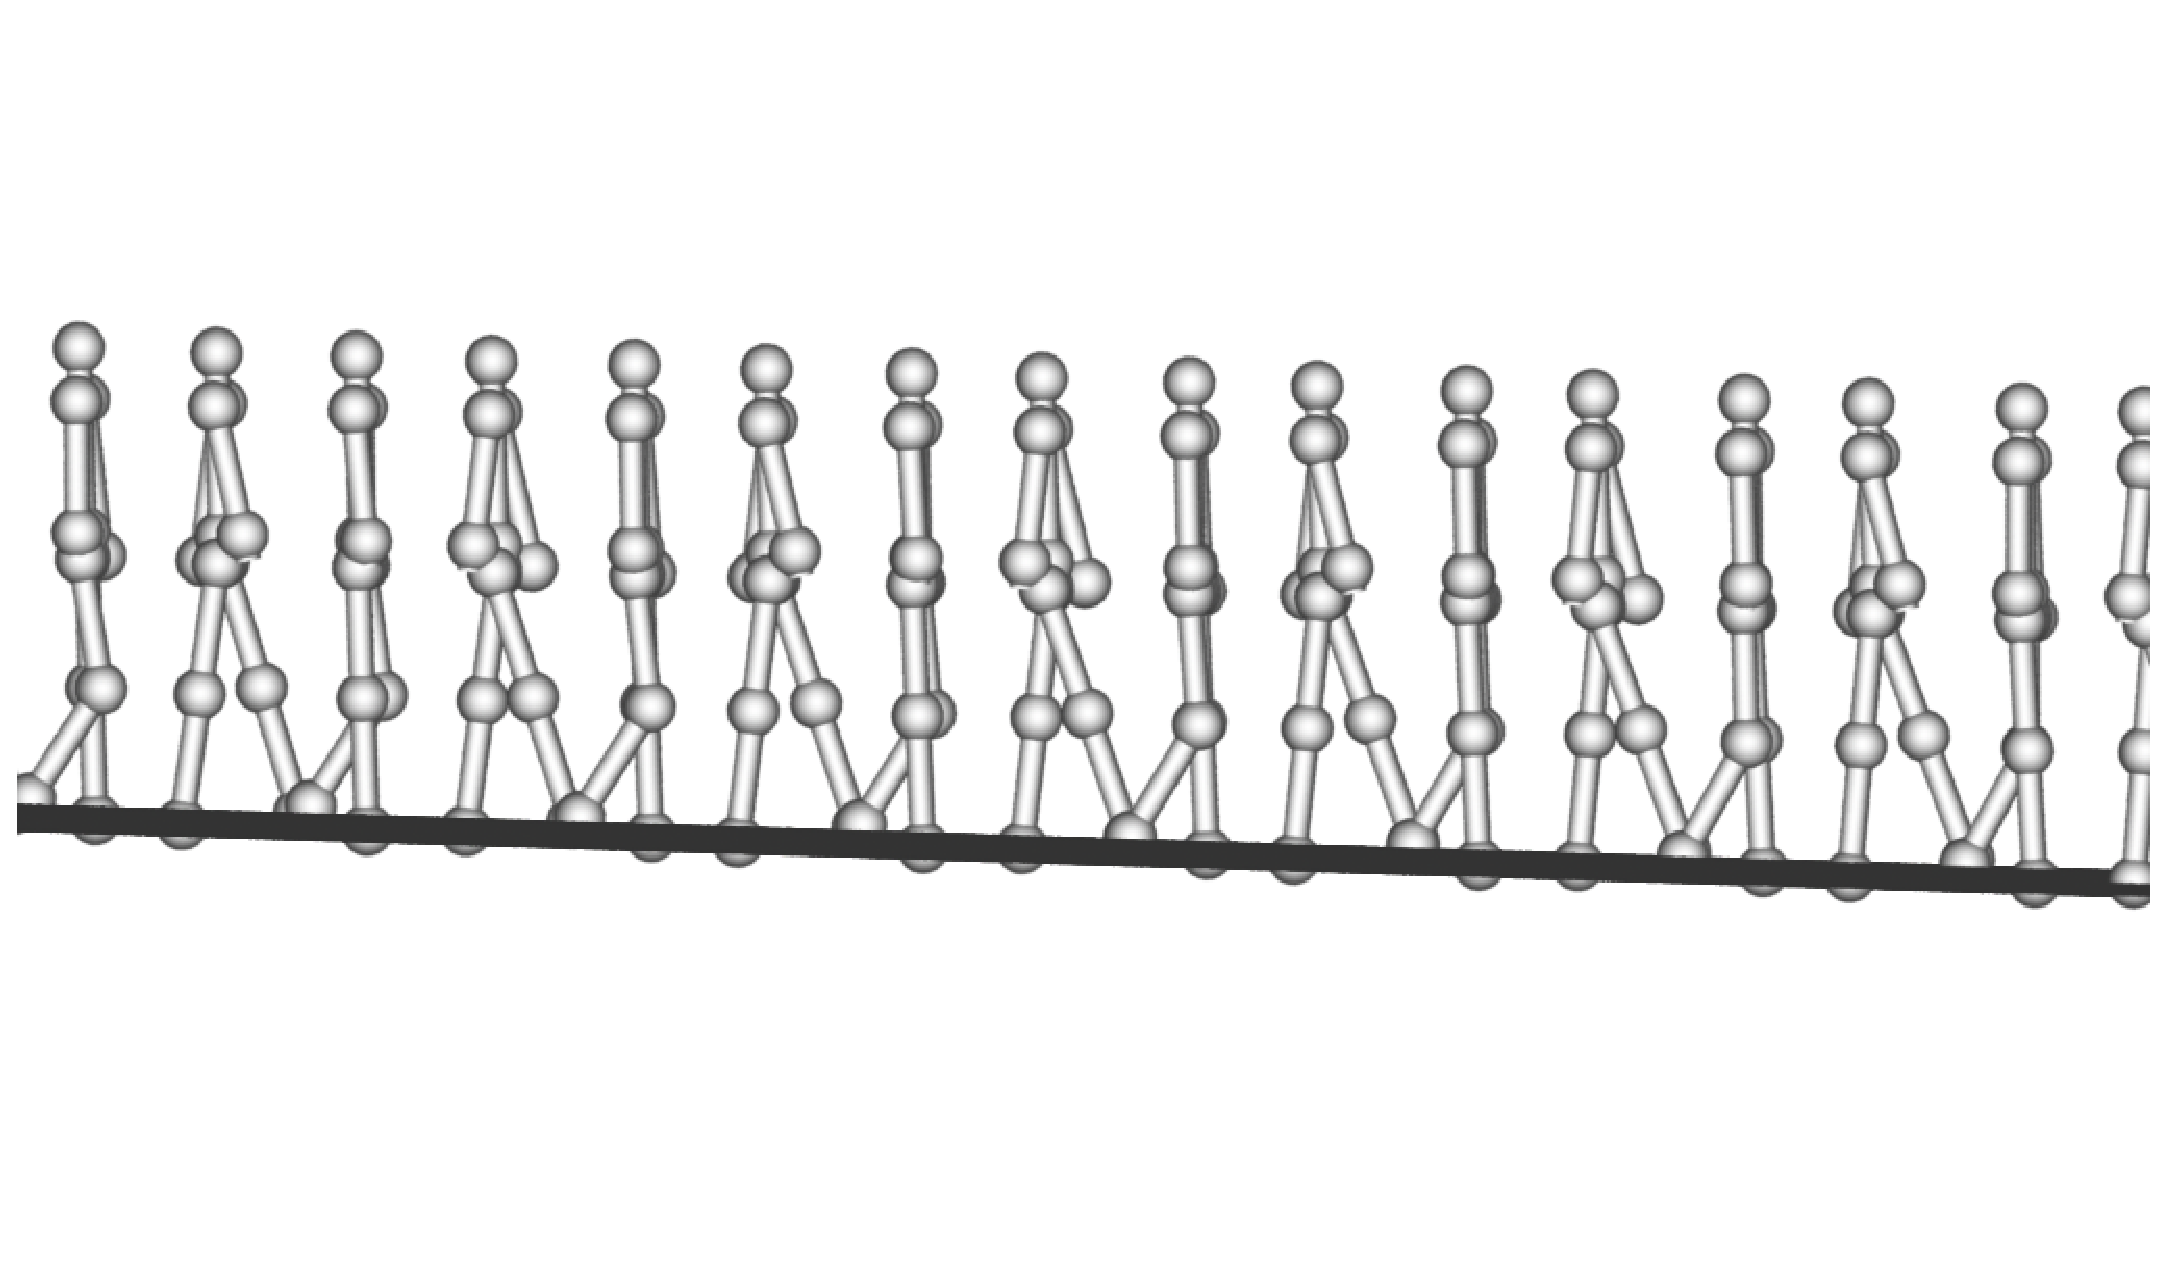
\includegraphics[width=0.7\textwidth]{Slope30}
    \caption{Gait On Slope 1} 
    \label{fig:ss1}
\end{center}
\end{figure}

\begin{figure}[!htbp]
  \begin{center}
      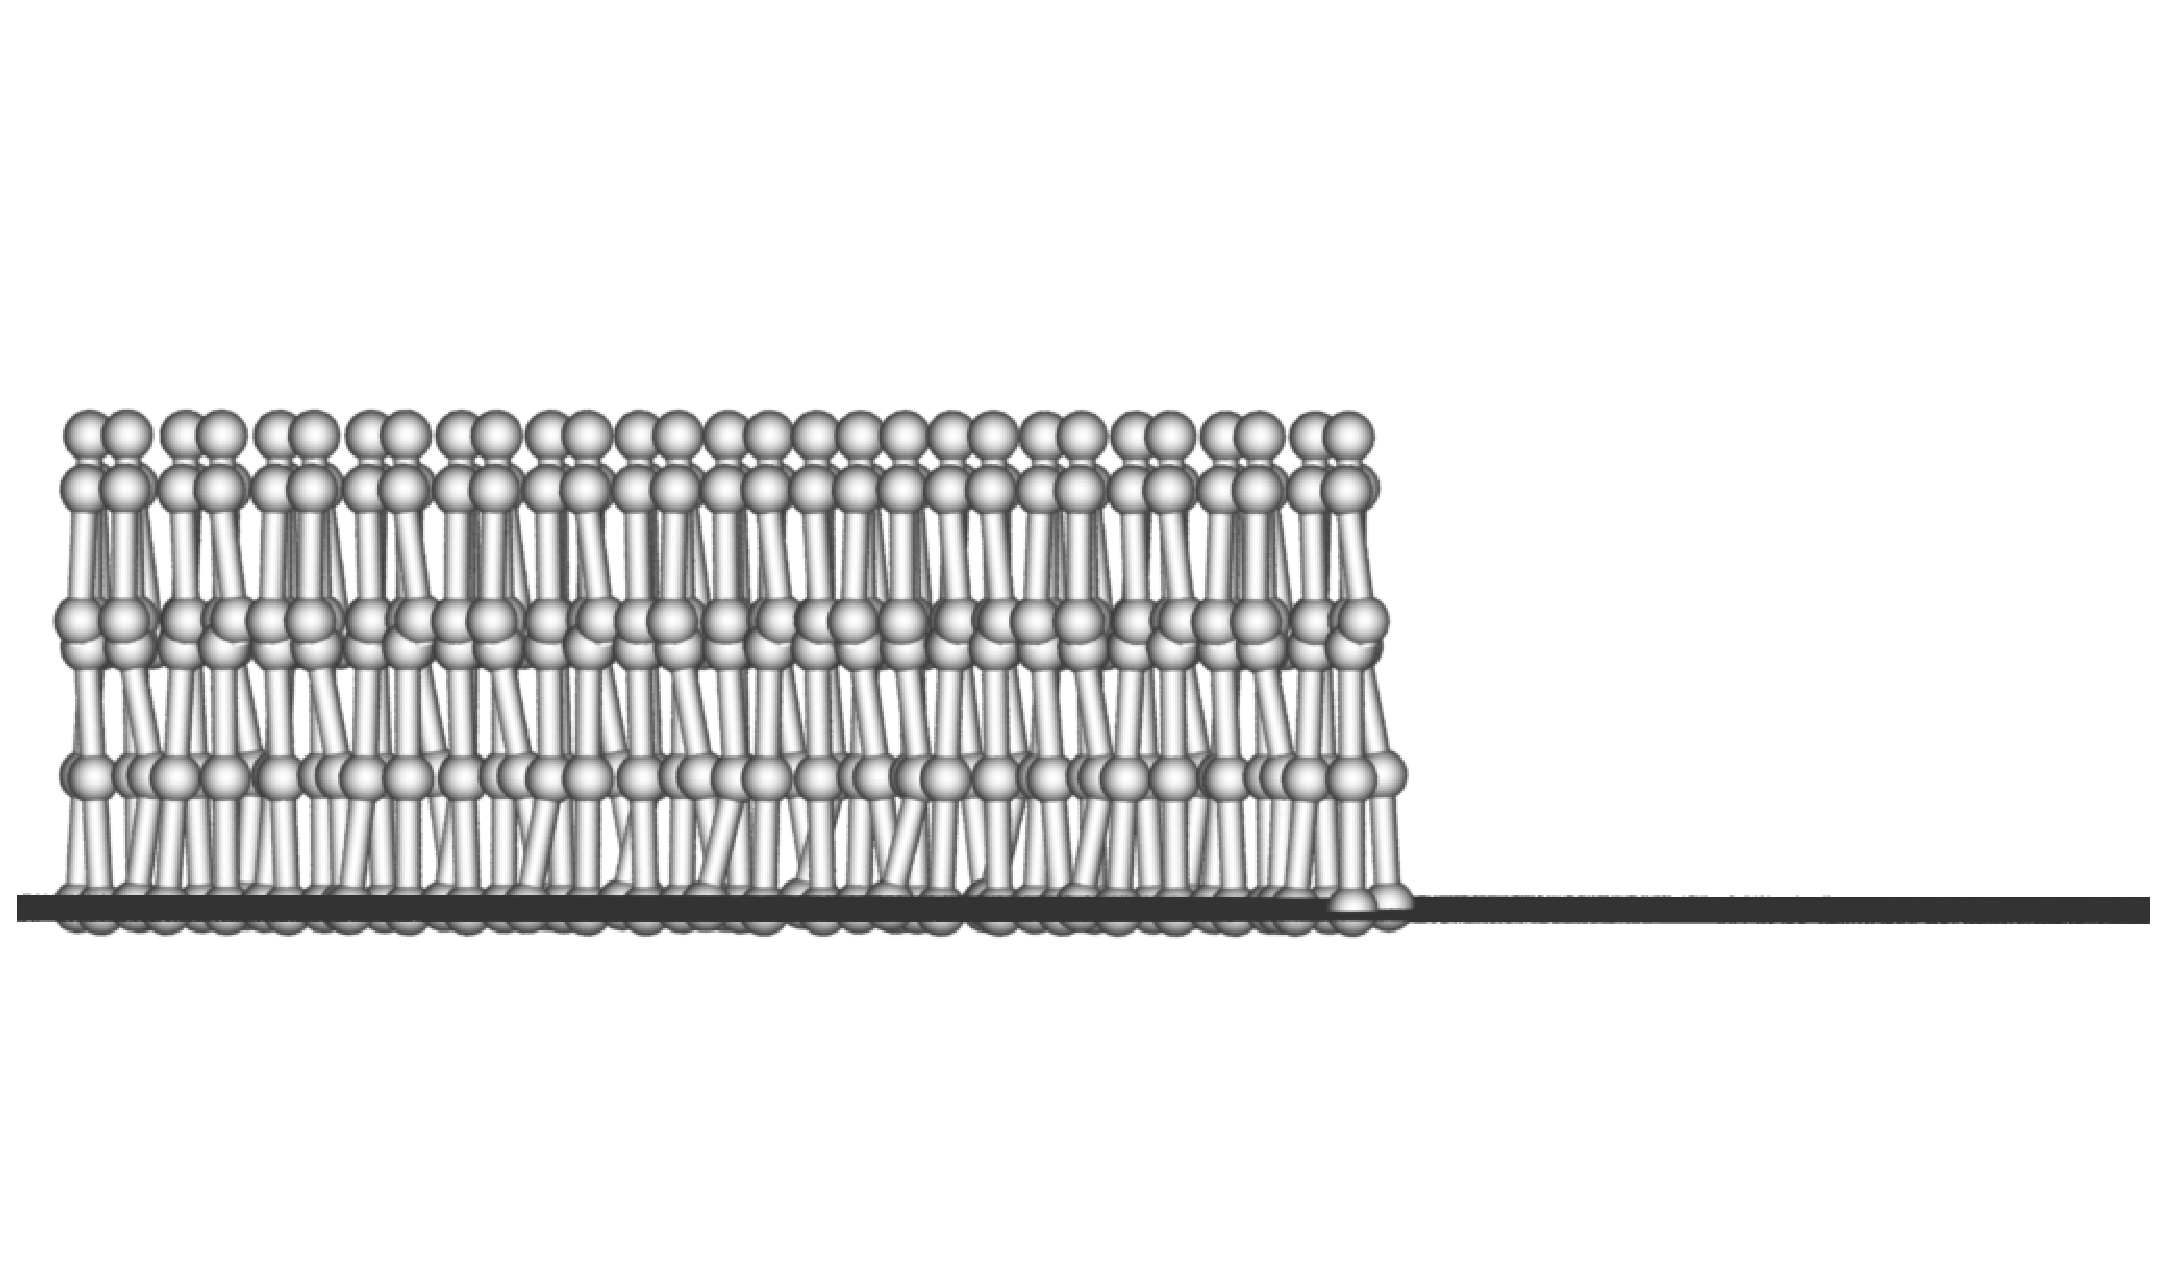
\includegraphics[width=0.7\textwidth]{Slope60}
    \caption{Gait On Slope 2}
    \label{fig:ss2}
\end{center}
\end{figure}

\begin{figure}[!htbp]
  \begin{center}
      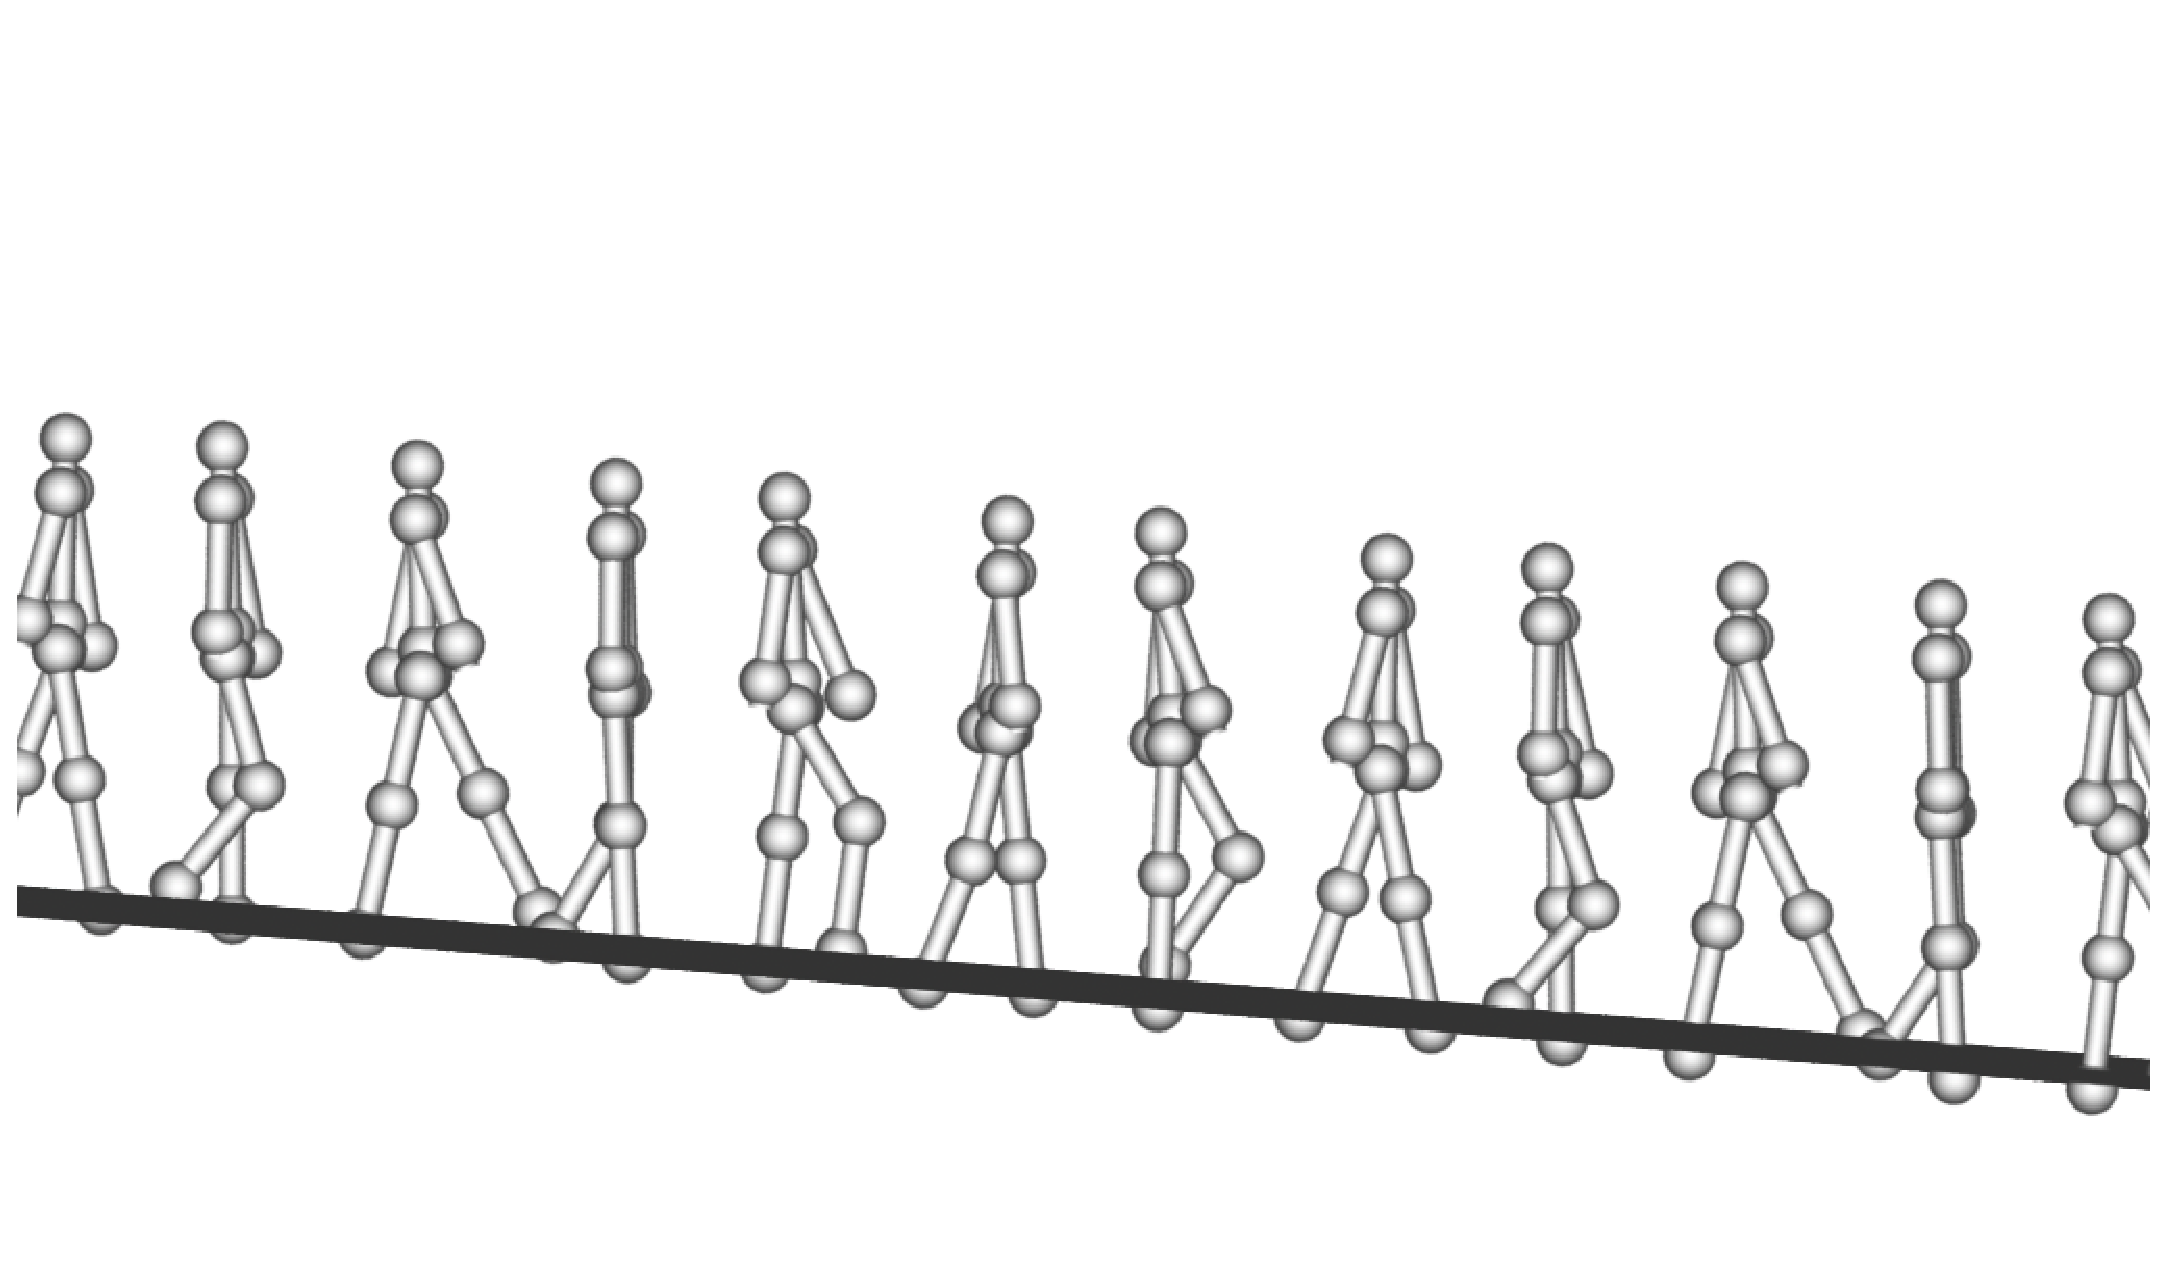
\includegraphics[width=0.7\textwidth]{Slope-20}
    \caption{Gait On Slope 3}
    \label{fig:ss3}
\end{center}
\end{figure}






\section{Local Motor Invariant Control}
Neural Oscillator boost the stability, sometimes stability becomes an limitation in motion.
For the walking example, if the basin of attraction covers the whole space, then the passive walker can't walk upslope.
If put the walker walk upslope, after a few steps, the passive walker will begin to walk backward downslope,as shown in Figure~\ref{fig:fig:withoutlocalcontroller}.
Also it is not convient to adjust the speed of walking.

Local Motor Invariant provides a mechanism to adapt motion according to the environment and application specific purpose.
Equation~\ref{eq:localcontrolwalking} describe walking with local control.


\begin{figure}[!htbp]
  \begin{center}
         $\begin{array}{cccc}
\includegraphics[width=1in]{UpFall/0001.eps}&
\includegraphics[width=1in]{UpFall/0051.eps}&
\includegraphics[width=1in]{UpFall/0101.eps}&
\includegraphics[width=1in]{UpFall/0151.eps}
\\
\includegraphics[width=1in]{UpFall/0201.eps}&
\includegraphics[width=1in]{UpFall/0251.eps}&
\includegraphics[width=1in]{UpFall/0301.eps}&
\includegraphics[width=1in]{UpFall/0351.eps}
\end{array}$
    \caption{Failure of walking upslope}
    \label{fig:localcontrolwalking}
\end{center}
\end{figure}

\begin{equation}
\label{eq:localcontrolwalking}
M(\mathbf{q}) \ddot{\mathbf{q}} + C(\mathbf{q,\qd})\dot{\mathbf{q}} + N(\mathbf{q}) = \ulocal
\end{equation}

\subsubsection{Group Actions}
Lie group actions are developed for two types of symmetry.
\begin{itemize}

\HiItem{Offset Action}.
Offset Action moves the phase plot horizontally, this will make the passive walking on terrain of different slope.
For the bipedal walking, the offset action is:
\[
\ulocal=N(q)-N(q+\ep)
\]
\HiItem{Speed Action}
Speed Action maintain the walking gait, but modify the walking speed.
The local control is:
\[  
\ulocal=(1-\ep^2)N
\]
\end{itemize}

The original system doest not have energy scalling symmetry.
Energy Scaling is approximate by a combined method discussed later.

Figure~\ref{fig:walkliegroupphase} demostrate different phase plot after appling lie group actions.
The red on is the original limit cycle.
Green one are apply speed action
Blue ones are applied  locol transform action


\begin{figure}[!htbp]
  \begin{center}
     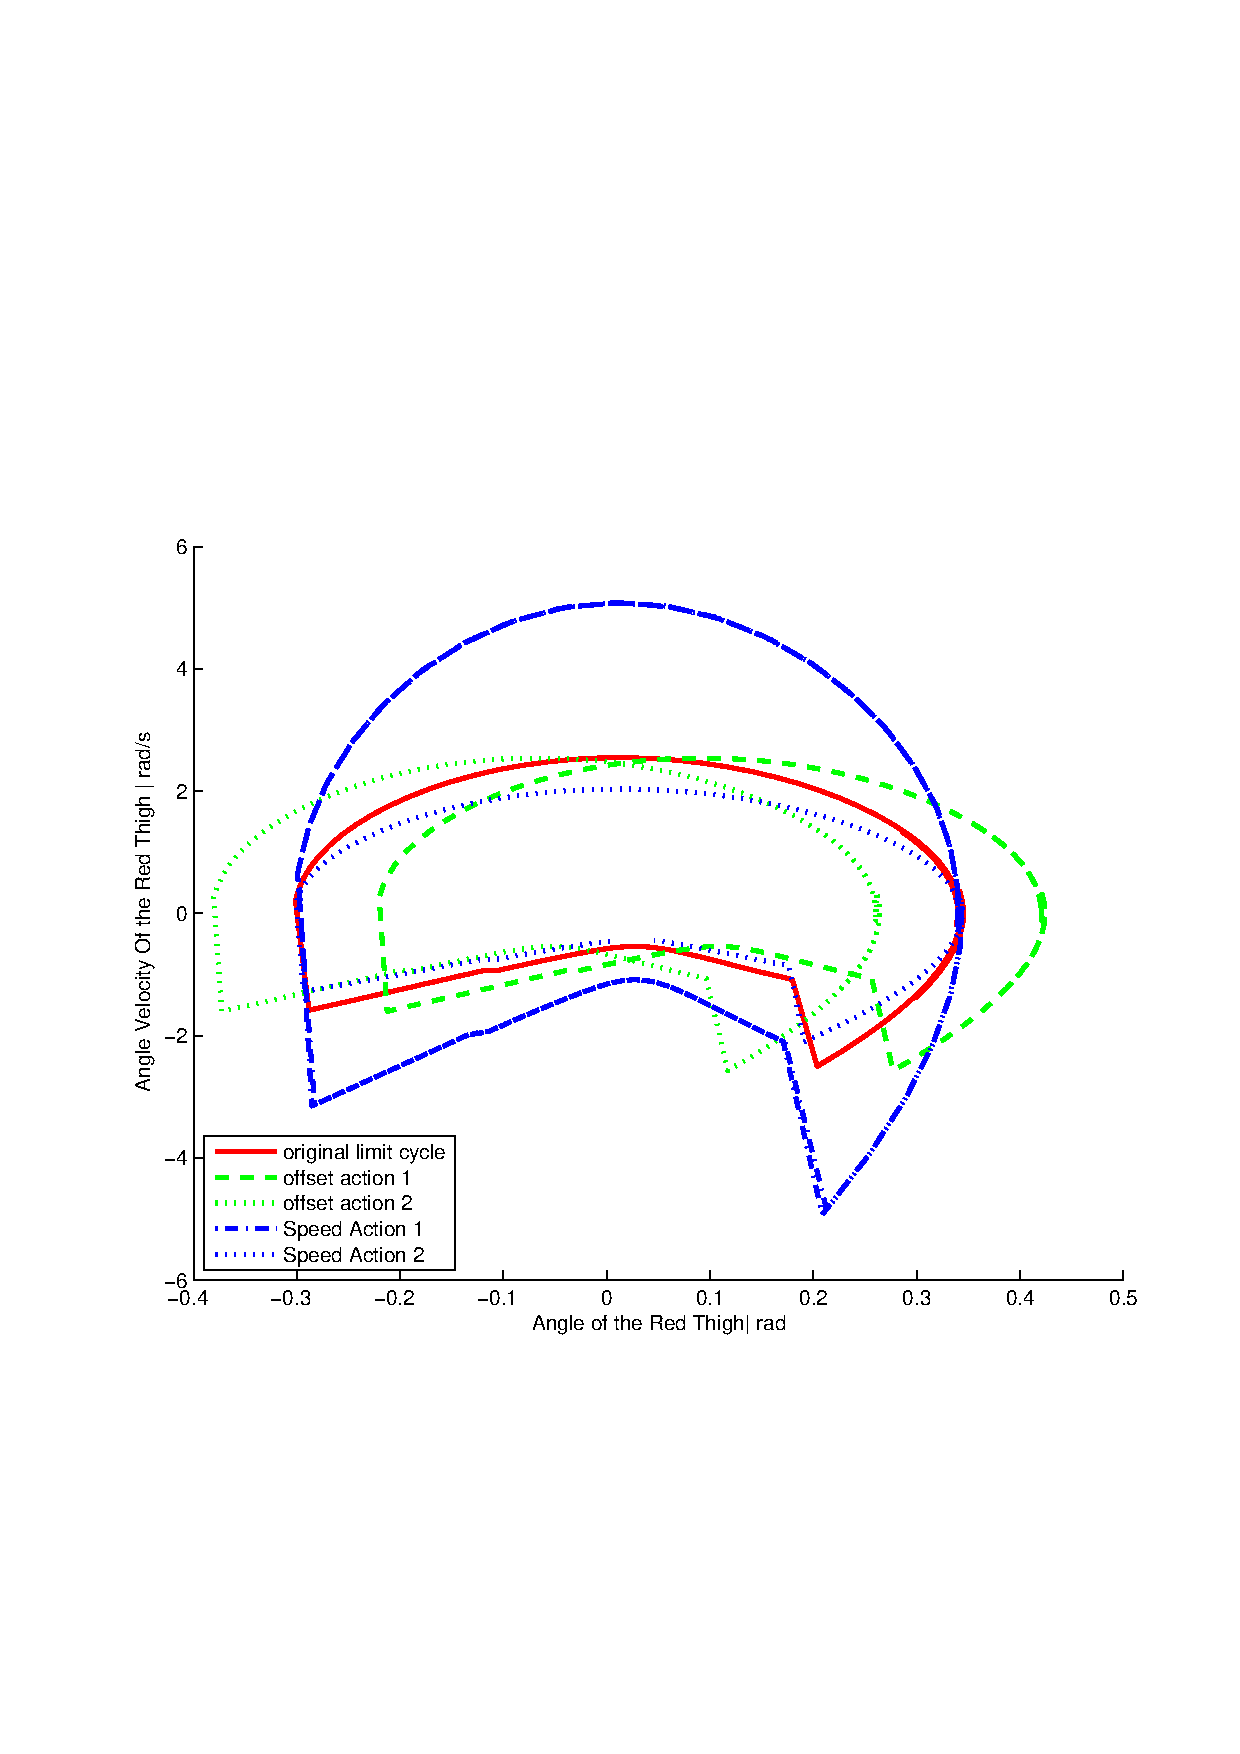
\includegraphics[width=0.7\textwidth]{LieGroupAction}
    \caption{Lie Group Actions on the Phase Plot}
    \label{fig:walkliegroupphase}
\end{center}
\end{figure}


Local Motor Invariant Control make it possible for the passive walker to walk upslope, as shown in Figure~\ref{fig:liegroupupslope}


\begin{figure}[!htbp]
  \begin{center}
      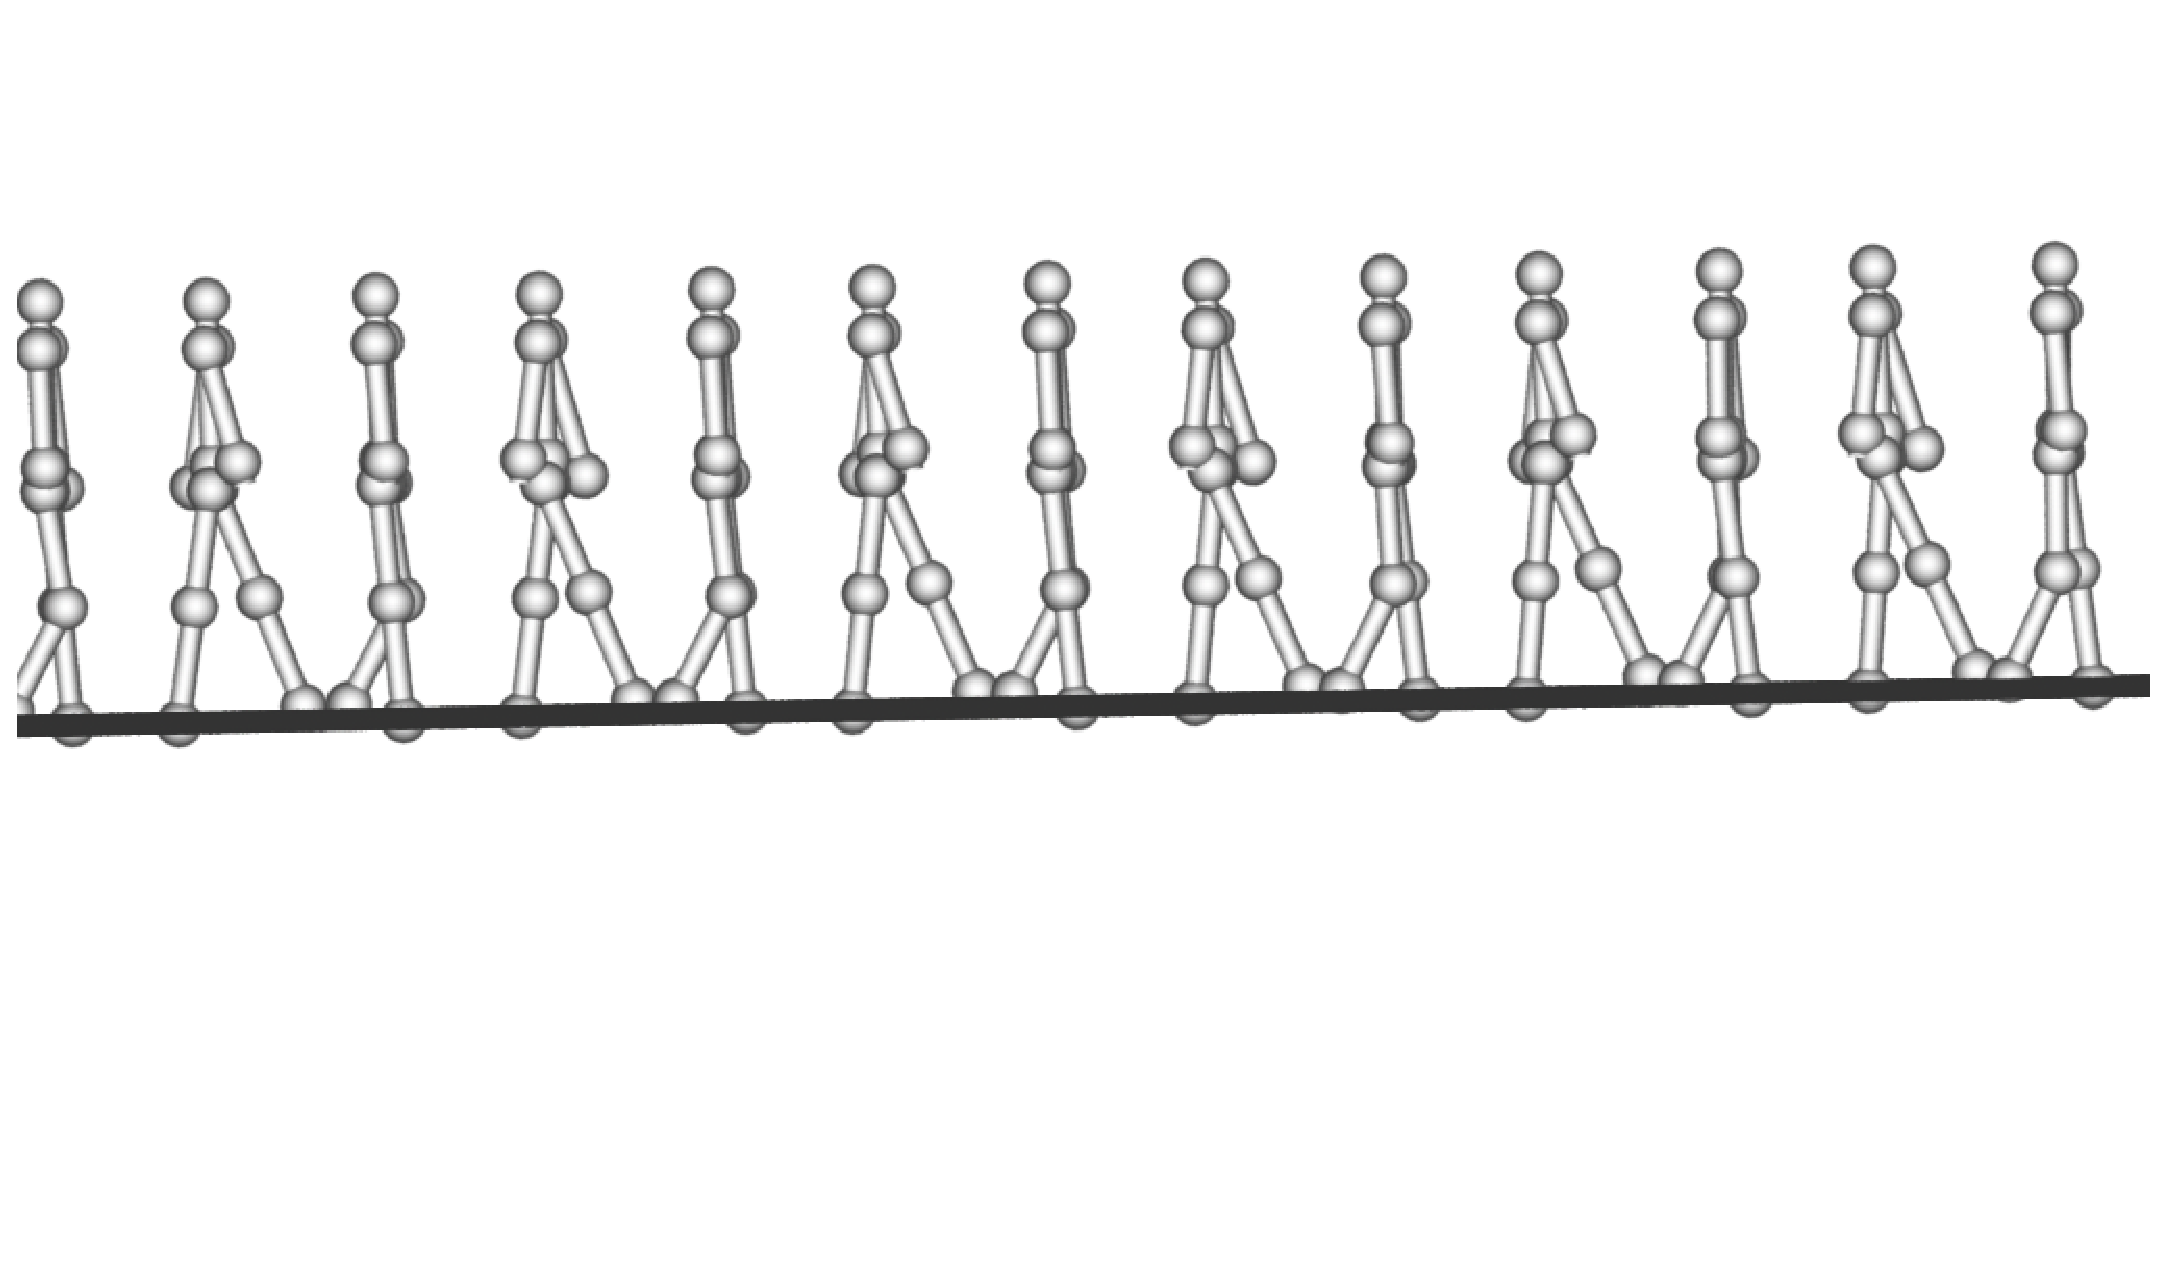
\includegraphics[width=0.7\textwidth]{LieUpslope}
    \caption{Upslope Gait Generate by Lie Group Action}
    \label{fig:liegroupupslope}
\end{center}
\end{figure}

\section{Control Combination}
Global Motor Invairant Control boost the walking stability, but sometimes can't the result motion can't meet application's needs.
Local Motor Invariant Control can adapt the walking to application purpose, but it can't boost the stability.
Combined the two controllers make it possbile to take advantage for the two methods.
The combined method is shown by Equation~\ref{eq:combinedcontrolwalking}
\begin{equation}
\label{eq:combinedcontrolwalking}
M(\mathbf{q}) \ddot{\mathbf{q}} + C(\mathbf{q,\qd})\dot{\mathbf{q}} + N(\mathbf{q}) = D\uout+\ulocal
\end{equation}


Animator can generate different gaits through neural oscillator, then transform the different gaits by lie group actions.
For animators, this method is efficient, natural looking and easy to use.
There are unlimited combination of adaptive gaits and transform action.
Some examples are shown in the following.


\subsection{Stepsize Adjust}
When the character walking down different slopes, steeper slope will result in a bigger stepsize as shown in Figure~\ref{DifferentSlope}, if Offset Lie Group actions is applyed, we can achieve different step gait on the constant slope.
Figure~\ref{fig:differentstepsizeonplaine} shows the gaits of different stepsize on the plane.

\begin{figure}[!htbp]
  \begin{center}
      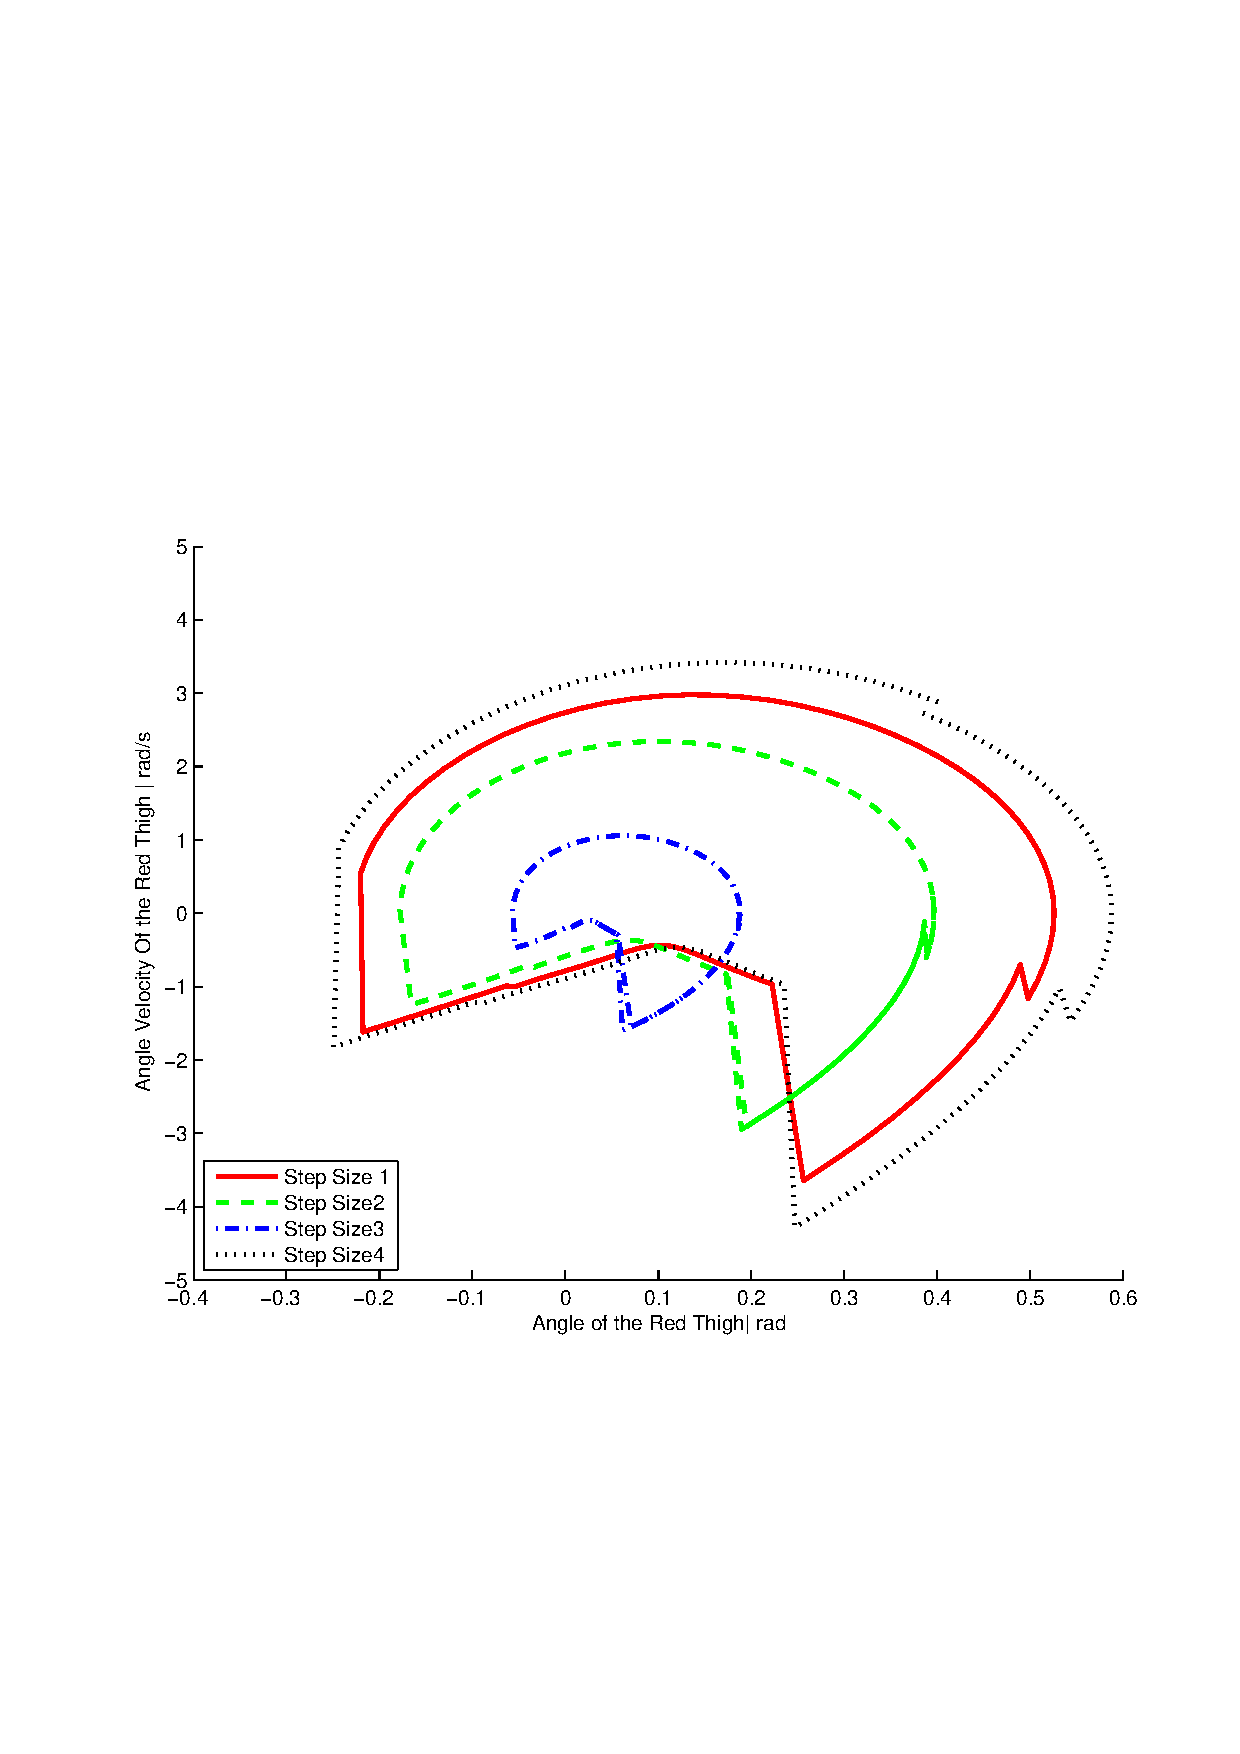
\includegraphics[width=0.7\textwidth]{DifferentStepSizeWalking}
    \caption{Limit Cycles of gaits of different step size}
    \label{fig:differentstepsizeonplaine}
\end{center}
\end{figure}



\begin{figure}[!htbp]
  \begin{center}
      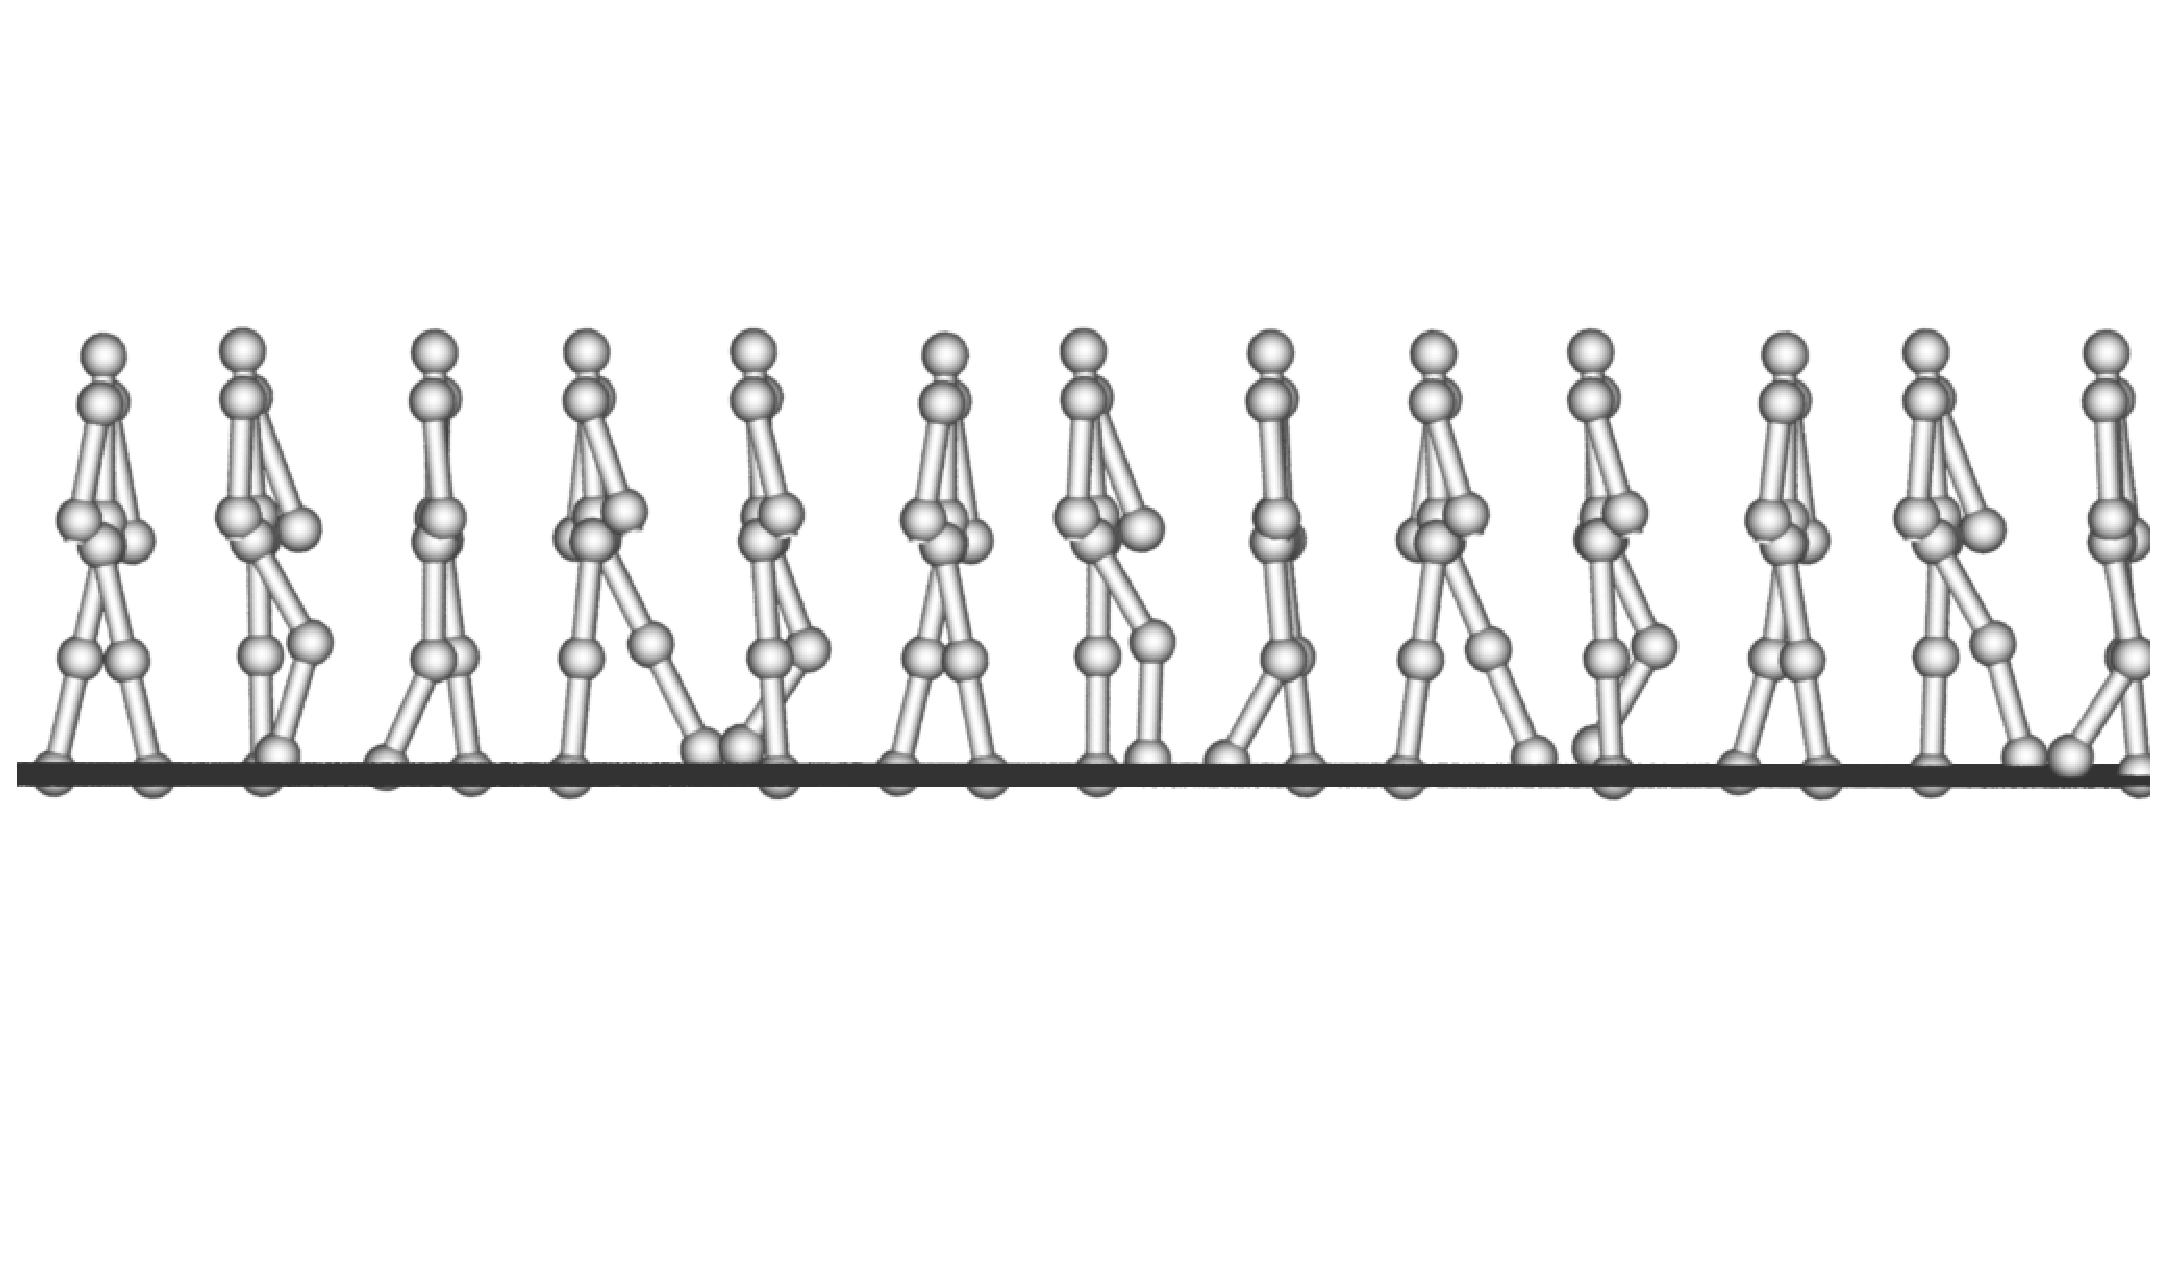
\includegraphics[width=0.7\textwidth]{stepsize1}
    \caption{gait with stepsize 1}
    \label{fig:ssp1}
\end{center}
\end{figure}

\begin{figure}[!htbp]
  \begin{center}
      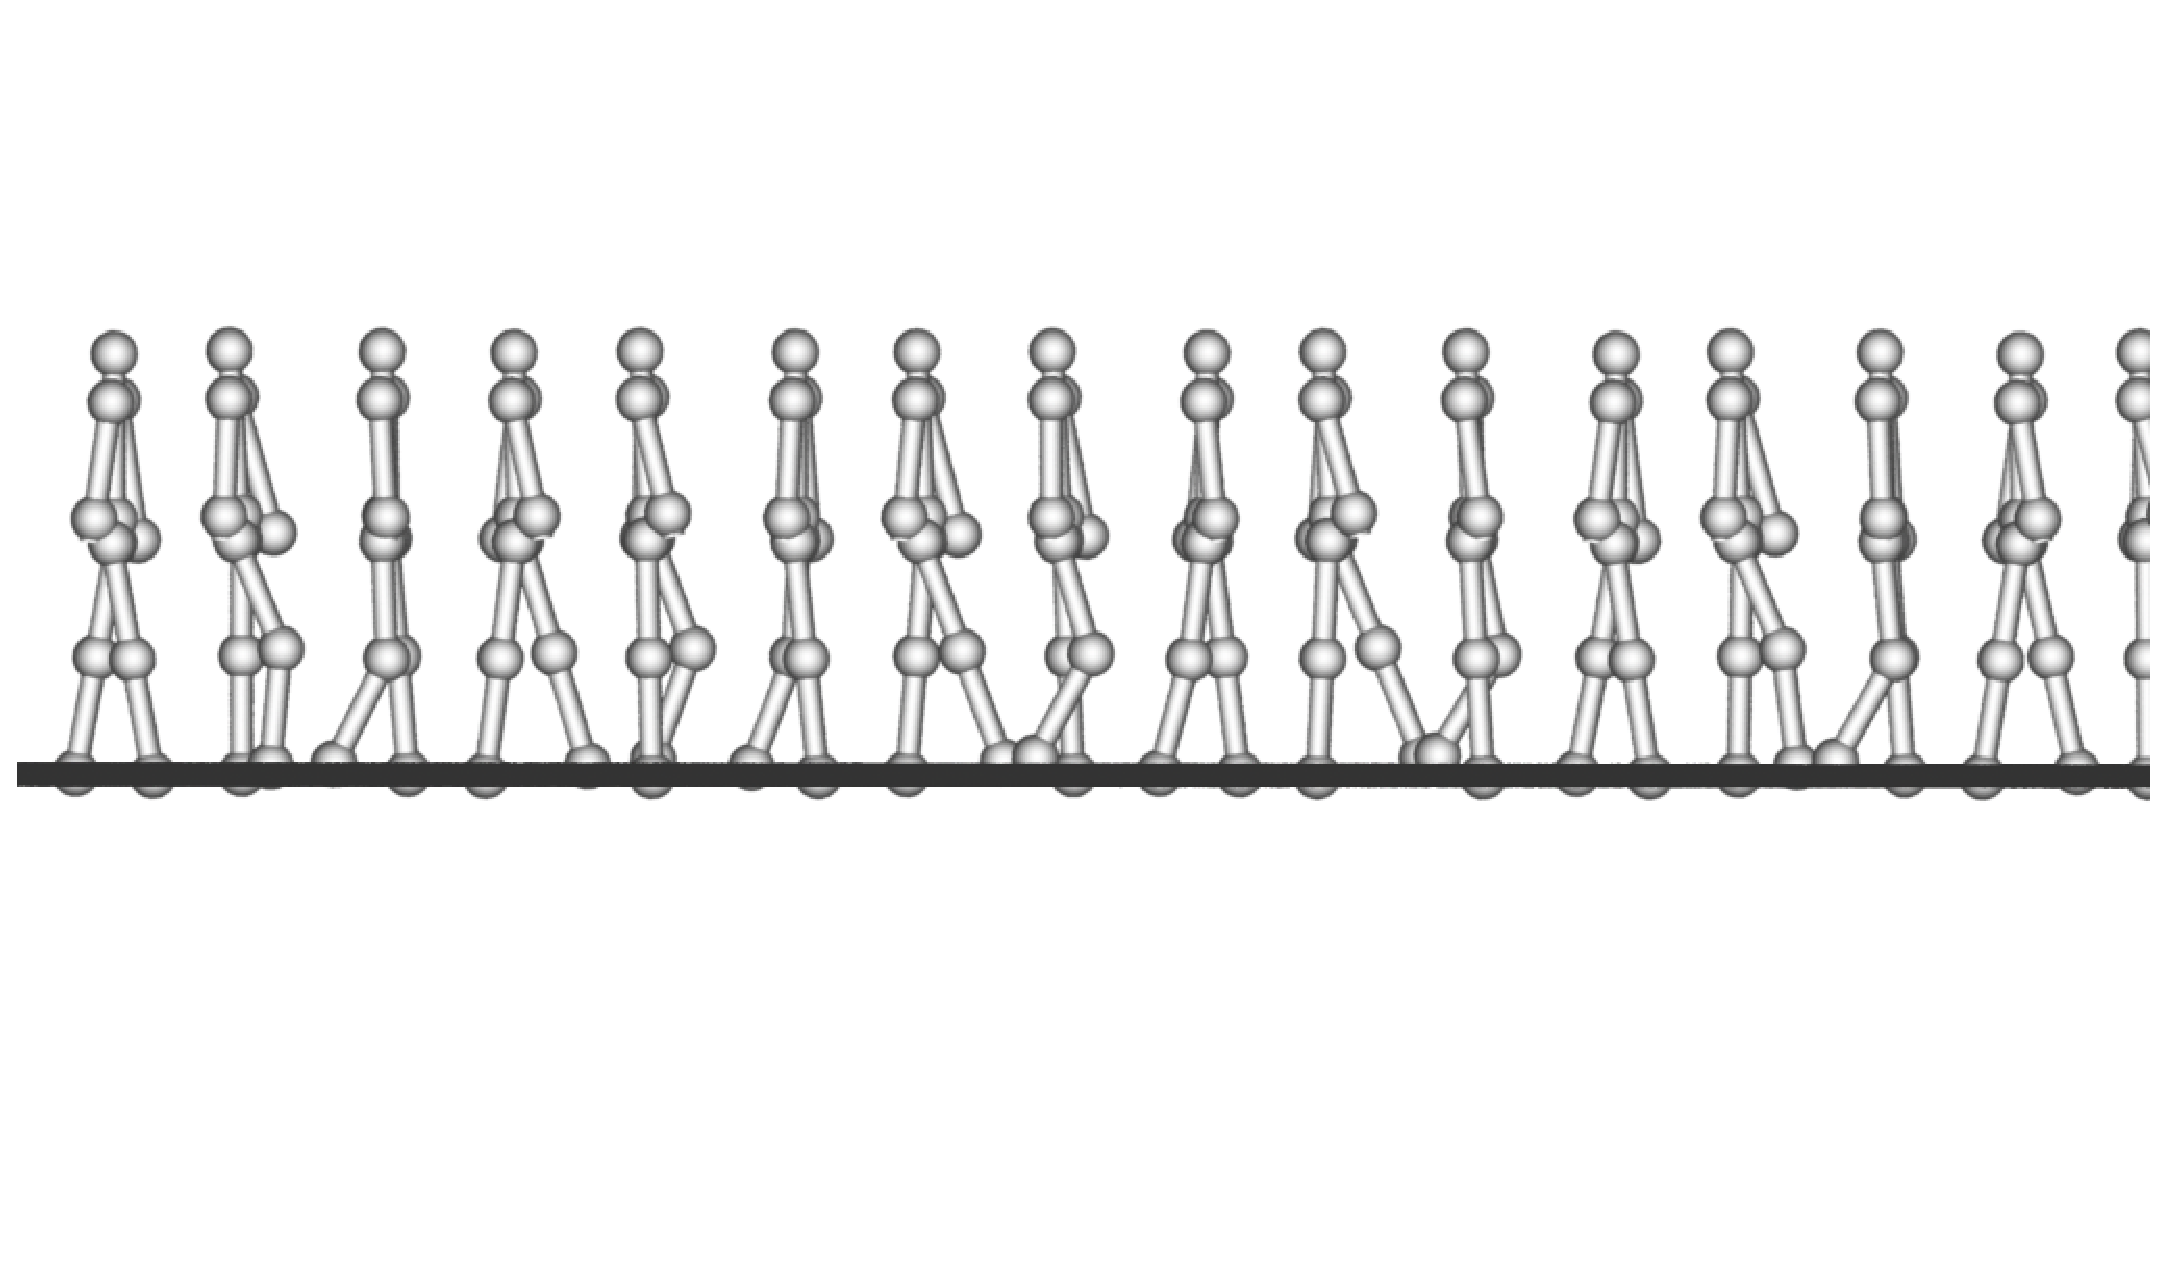
\includegraphics[width=0.7\textwidth]{stepsize2}
    \caption{gait with stepsize 2}
    \label{fig:ssp2}
\end{center}
\end{figure}

\begin{figure}[!htbp]
  \begin{center}
      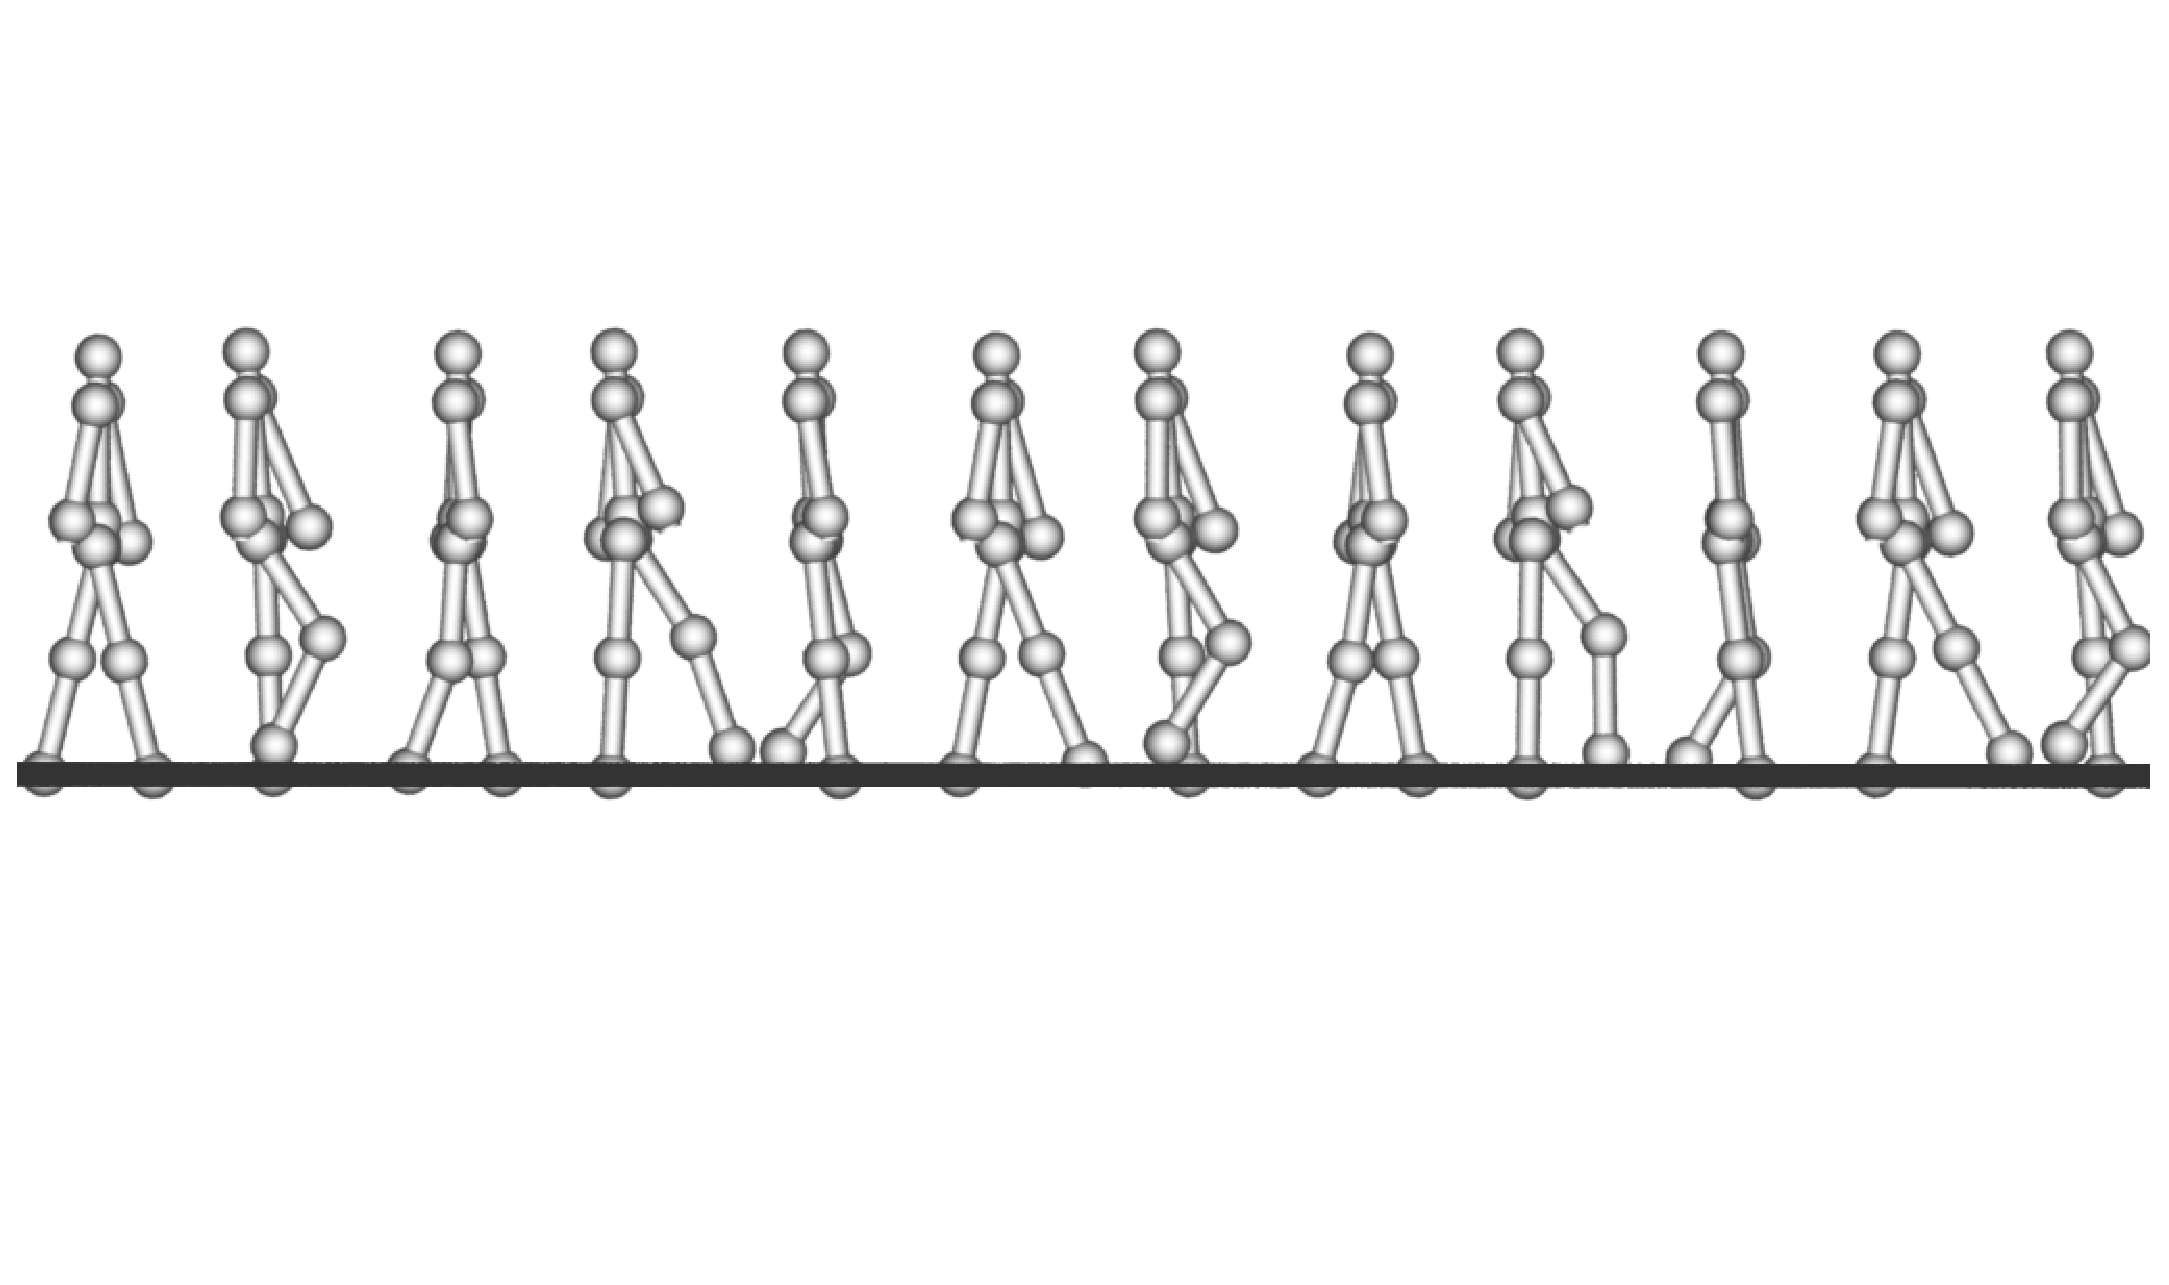
\includegraphics[width=0.7\textwidth]{stepsize4}
    \caption{gait with stepsize 4}
    \label{fig:ssp3}
\end{center}
\end{figure}







\subsection{Varying Slopes}
Neural Oscillator can maintain walking by varing slopes, but can't make character walking upslope.
Lie Group action allow the character walking up a slope with a constant angle, but varying the slope will result walking failure.
Combined the two methods, the passive walker can walk varying upslope.


The control strategy it is straigt forward, lie group action is maintained on each plane, during slope transition, controller look ahead and set the lie group action for to walking on the slope for the next step.
At transtion, the state will moved far away from the stable limit cycle, need a few steps to converge to the limit circle.
This result gait adjustment, sometimes, character will take a few small steps and increase it to normal steps.


Figure~\ref{fig:vp1} and Figure~\ref{fig:vp2} show the gaits on smooth slopes.
The phase plot of gaits of Figure~\ref{fig:vp1} is shown in Figure~\ref{fig:vp2phas} 

\begin{figure}[!htbp]
  \begin{center}
      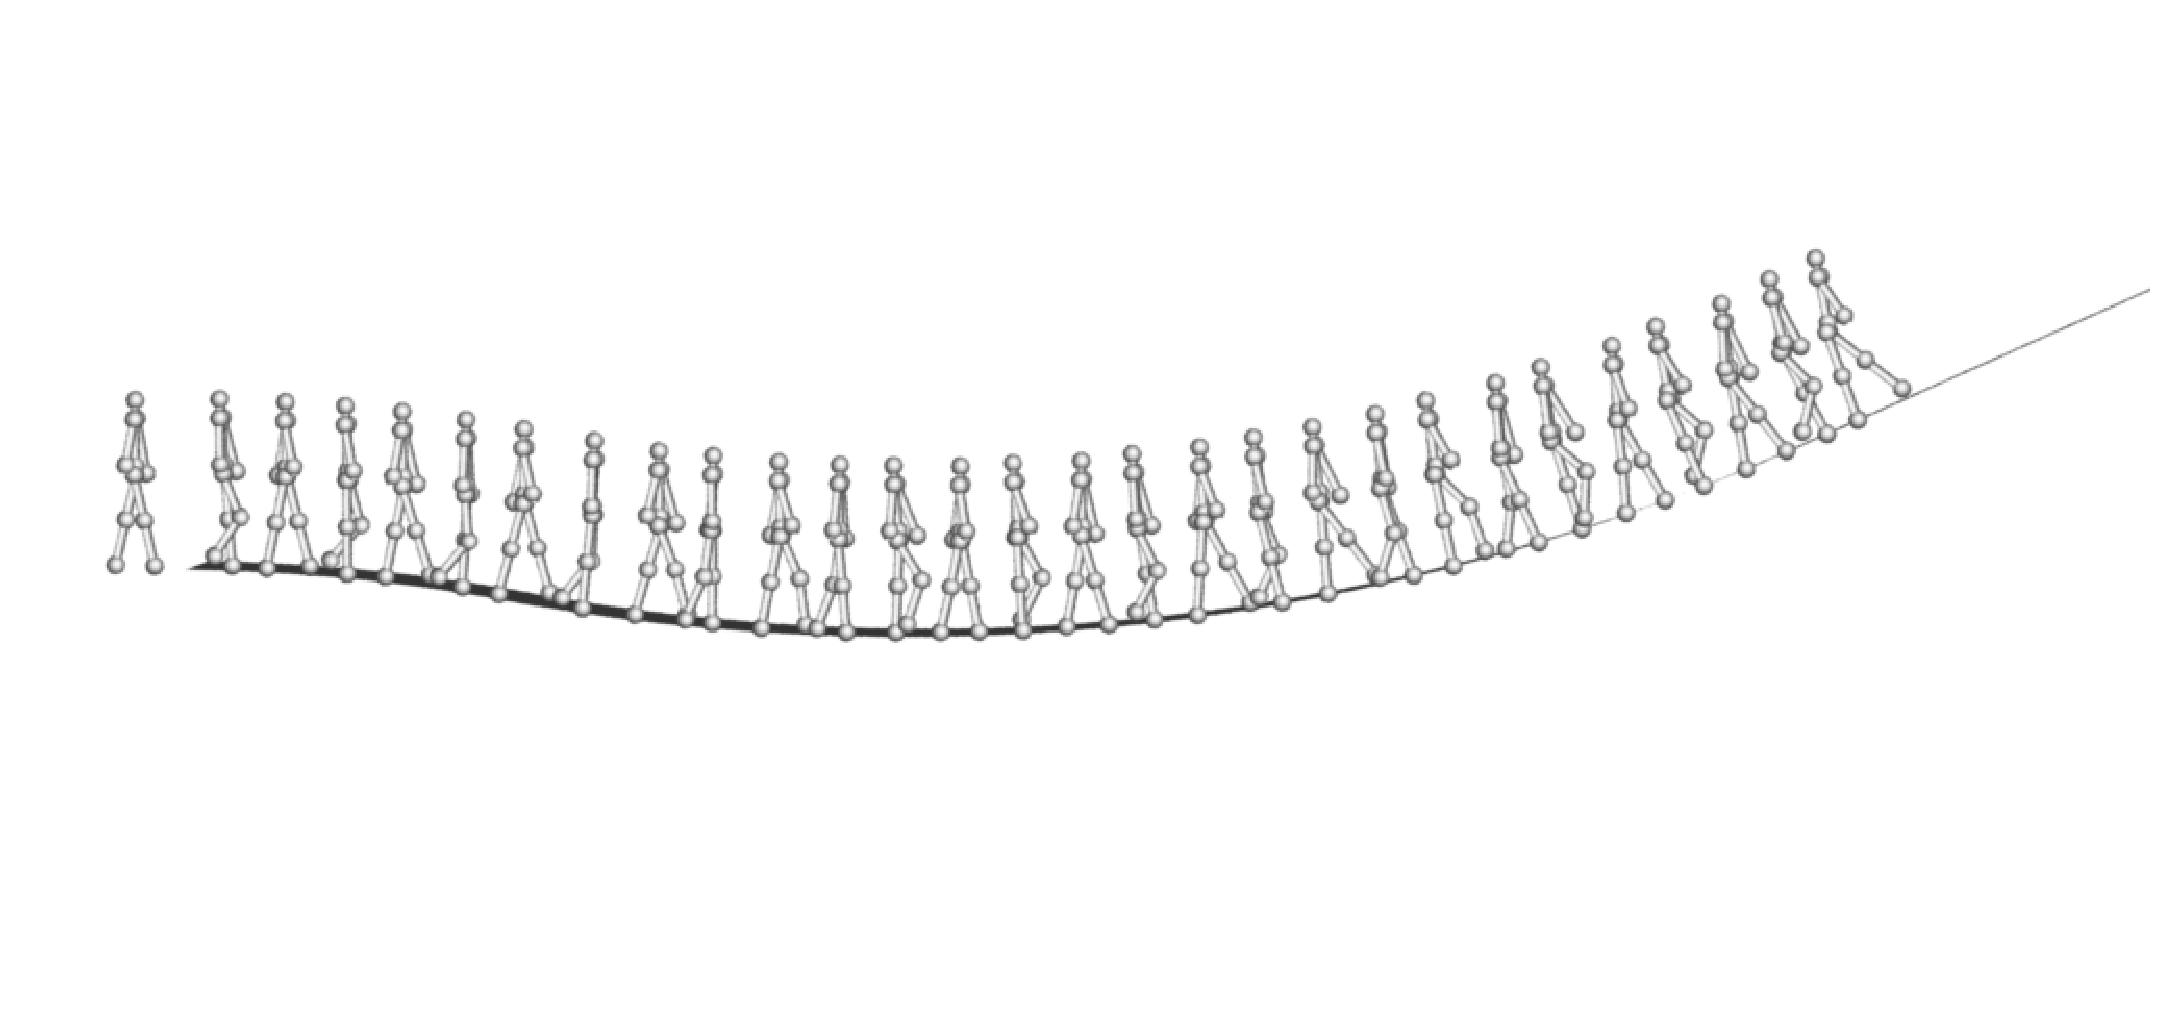
\includegraphics[width=0.7\textwidth]{vslope2}
    \caption{Continous Varying Slope}
    \label{fig:vp1}
\end{center}
\end{figure}


\begin{figure}[!htbp]
  \begin{center}
      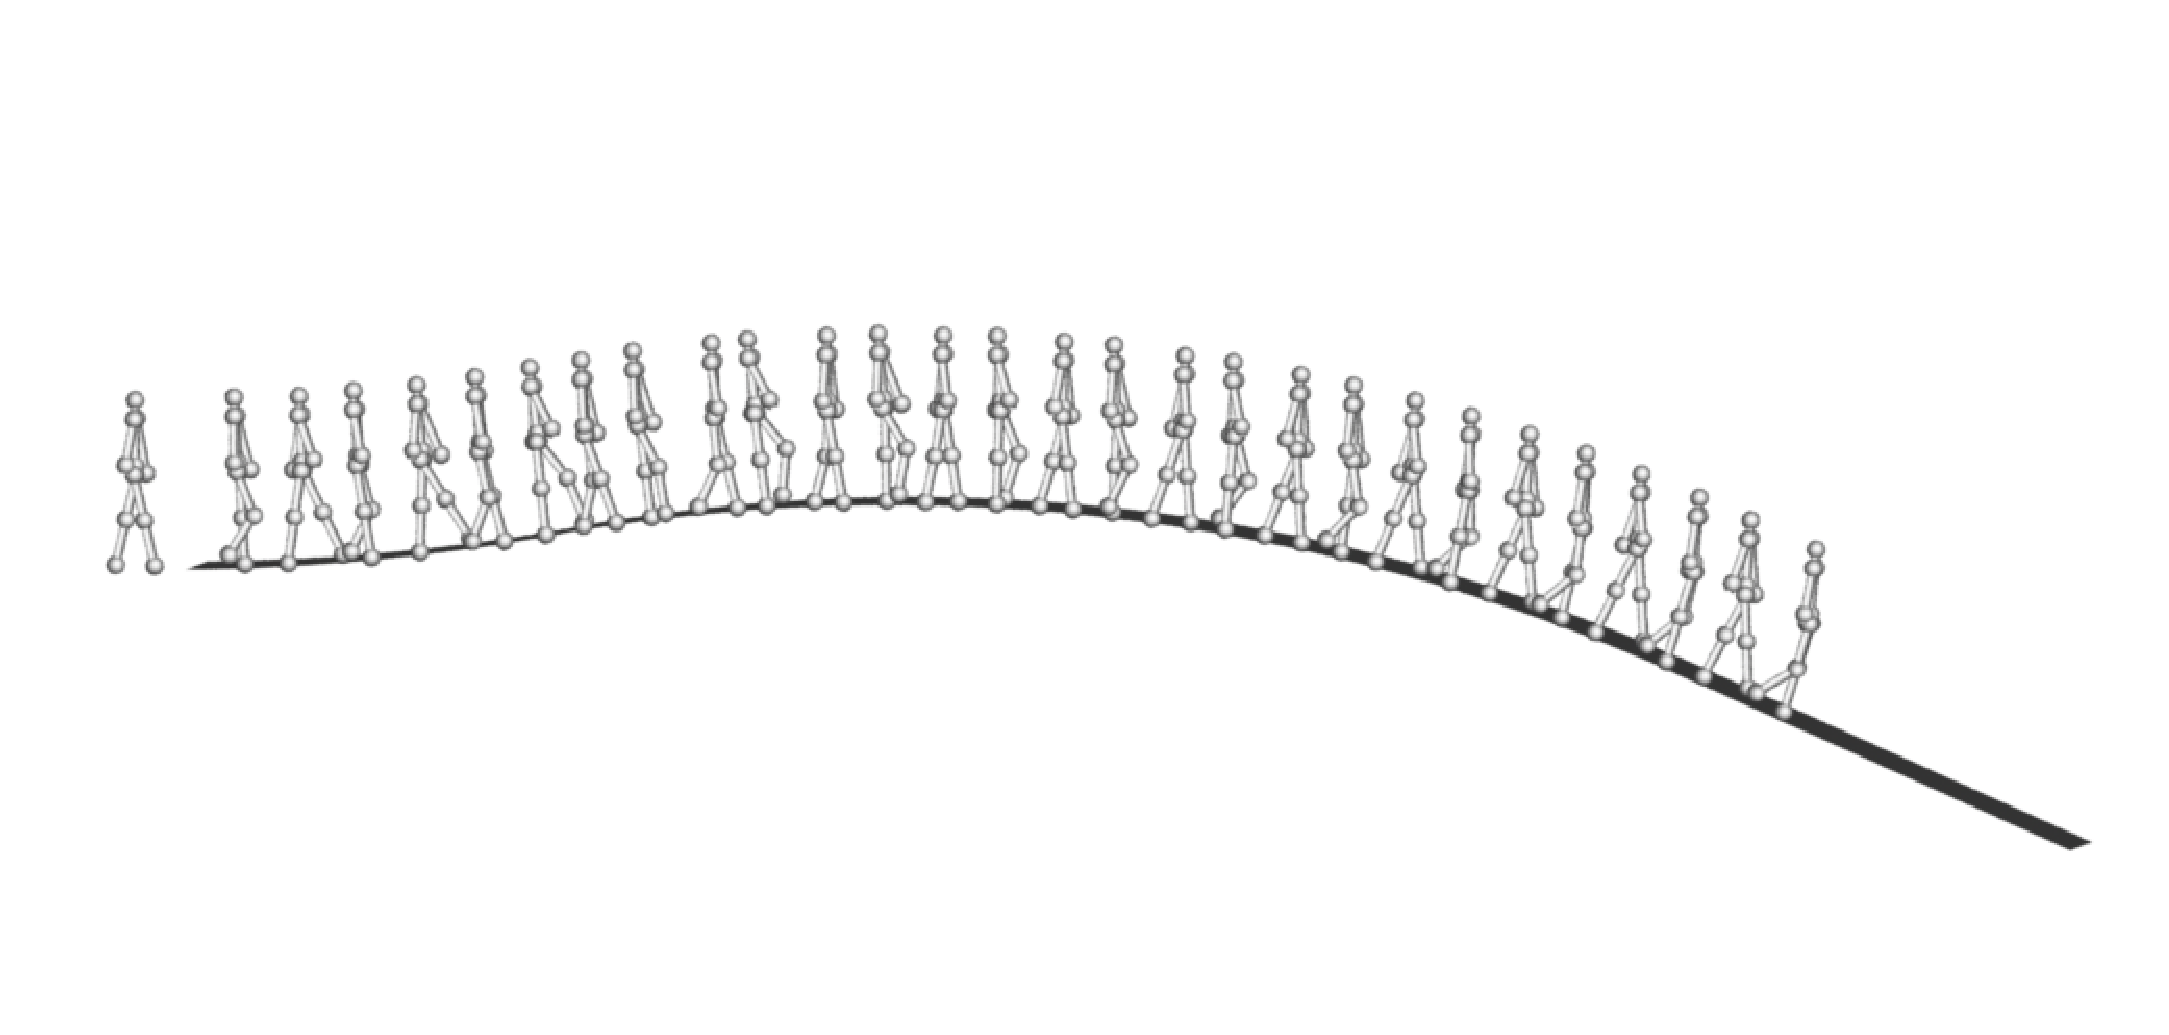
\includegraphics[width=0.7\textwidth]{vslope3}
    \caption{Continous Varying Slope}
    \label{fig:vp2}
\end{center}
\end{figure}


\begin{figure}[!htbp]
  \begin{center}
      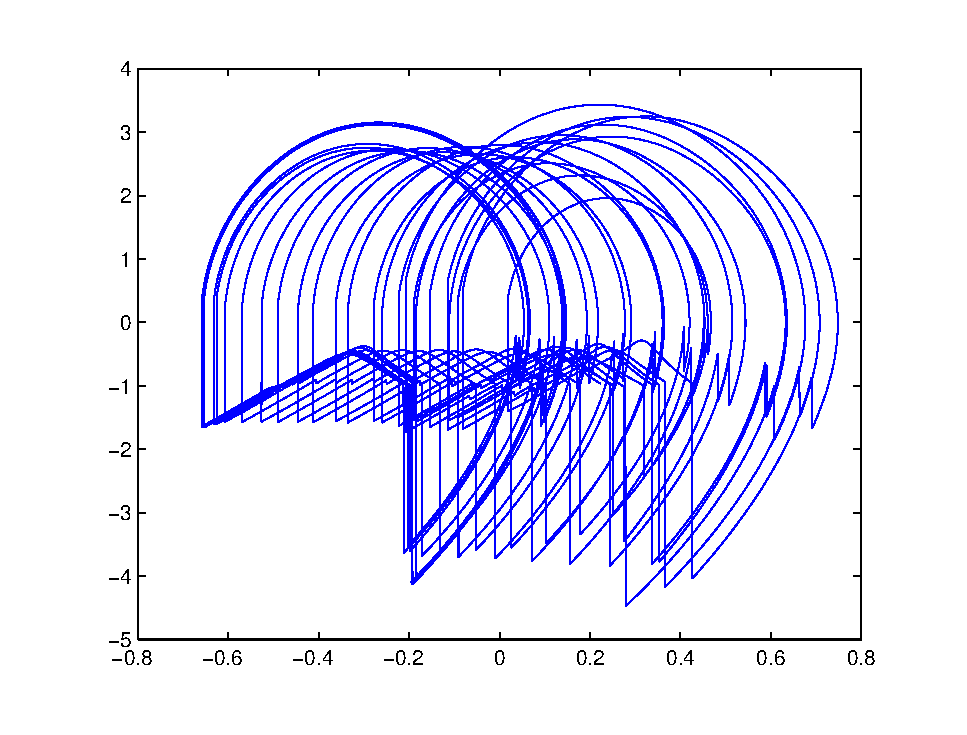
\includegraphics[width=0.7\textwidth]{vslope3phaseplot}
    \caption{Continous Varying Slope}
    \label{fig:vp2phas}
\end{center}
\end{figure}



Figure~\ref{fig:nonsmoothterrain1}, Figure~\ref{fig:nonsmootterrain2} show gaits on none smooth terrain.
And the phase plot is shown in Figure~\ref{fig:diffterrain1phase}.
Another Terrain is shown in Figure~\ref{fig:diffterrain2}.








\begin{figure}[!htbp]
  \begin{center}
      \includegraphics[width=0.7\textwidth]{terrain2}
    \caption{Nonsmooth Terrain }
    \label{fig:nonsmoothterrain1}
\end{center}
\end{figure}

\begin{figure}[!htbp]
  \begin{center}
      \includegraphics[width=0.7\textwidth]{terrain3}
    \caption{Nonsmooth Terrain coloured}
    \label{fig:nonsmootterrain2}
\end{center}
\end{figure}


\begin{figure}[!htbp]
  \begin{center}
    \includegraphics[width=0.7\textwidth]{Terrain3PhaseDifferentColor}
    \caption{The Phase Plot of nonsmooth terrain}
    \label{fig:diffterrain2}
\end{center}
\end{figure}






